%******************************FORMATIERUNG****************************************
\documentclass[a4paper, 12pt]{article}
\usepackage{scrpage2}
\usepackage{todonotes}
\usepackage{amssymb}
\usepackage{amsmath}
\usepackage{esvect}
\usepackage{caption}
\pagestyle{scrheadings}
\clearscrheadfoot
\setheadsepline{.5pt}
\setfootsepline{.5pt}
\automark[section]{chapter}
\ihead{\headmark}
\ohead{\pagemark}
\usepackage[ngerman]{babel}
\usepackage[utf8]{inputenc}
\usepackage{graphicx}
\usepackage[space]{grffile}
\usepackage{setspace}
\usepackage[T1]{fontenc}
\usepackage[section]{placeins}
\usepackage{listings}
\renewcommand{\lstlistingname}{Source Code}	
\definecolor{lsgreen}{rgb}{0,.5,0}
\definecolor{lsred}{rgb}{.7,0,0}
\definecolor{lsorange}{rgb}{.9,.5,0}
\definecolor{lsgray}{rgb}{.5,.5,.5}
\lstloadlanguages{[Sharp]C}
\lstset{
	frame=tb,
	aboveskip=10mm,
	belowskip=5mm,
	showstringspaces=false,
	columns=flexible,
	captionpos=b,
	basicstyle={\scriptsize\ttfamily},
	numbers=left,
	numberstyle=\tiny\color{lsgray},
	keywordstyle=\color{blue},
	commentstyle=\color{lsorange},
	stringstyle=\color{lsgreen},
	breaklines=true,
	breakatwhitespace=true,
	rulecolor=\color{lsgray},
	xleftmargin=7mm,
	tabsize=3
}
\newcommand{\changefont}[3]{
\fontfamily{#1} \fontseries{#2} \fontshape{#3} \selectfont}
\usepackage{datetime}
\newdateformat{monthyeardate}{%
  \monthname[\THEMONTH] \THEYEAR}
\usepackage{geometry}
\geometry{verbose,a4paper,tmargin=30mm,bmargin=30mm,lmargin=35mm,rmargin=25mm}
\usepackage[numbers,square]{natbib}
\usepackage[
	breaklinks=true,
	pdfauthor={Laura Anger, Vera Brockmeyer, Britta Boerner, Anna Bolder},
	pdftitle={Interaction Lab},
	pdftoolbar=true,
	%pdfsubject={},
	colorlinks=true,
	linkcolor=blue,
	citecolor=blue,
	urlcolor=blue,
	linktocpage=true
	]{hyperref}
\usepackage{algorithmicx}
\usepackage{multicol}
\usepackage{multirow}
\usepackage[ruled]{algorithm}
\usepackage{algpseudocode}
\usepackage{pdfpages}
\usepackage[
	font=small,
	labelfont=bf, 
	format=plain,
	indention=1cm
	]{caption}
\setlength{\parindent}{0pt} 
\setlength{\parskip}{.5em}
\usepackage{color}
\definecolor{myColor}{rgb}{0.8,0.8,0.8}
\newcommand{\Absatzbox}[1]{\parbox[0pt][2em][c]{0cm}{}}
\usepackage{listings}
\usepackage{tabularx}

%Laura: Paragraphen werden auch nummeriert. Können wir auch weglassen
%\usepackage{titlesec}
%\setcounter{secnumdepth}{4}
%\titleformat{\paragraph}
%{\normalfont\normalsize\bfseries}{\theparagraph}{1em}{}
%\titlespacing*{\paragraph}
%{0pt}{3.25ex plus 1ex minus .2ex}{1.5ex plus .2ex}

%*****************************ENDE FORMATIERUNG****************************************

\begin{document}
%\linespread{1.2}
%\changefont{ppl}{m}{n}

%INHALTSVERZEICHNIS
%\pagenumbering{arabic}
%\input{main/Inhaltsverzeichnis.tex}

\thispagestyle{empty}
\begin{center}
	
\includegraphics[width=5cm]{Images/logo_TH}\\[12ex]
	{\Huge\textbf{Project Documentation}}\\[8ex]
	\rule{.8\textwidth}{.2pt}
	{\Large\\[1ex] \textbf{Interaction Lab}}\\
	\rule{.8\textwidth}{.2pt}\\[10ex]
	written by\\[2ex]
	\begin{tabular}{ll}
		Vera Brockmeyer &(Matrikelnr. 11077082)\\
		Anna Bolder &(Matrikelnr. 11083451)\\
		Britta Boerner &(Matrikelnr. 11070843)\\
		Laura Anger &(Matrikelnr. 11086356)\\ 
	\end{tabular}\\[10ex]
	\textbf{Interactive Systems in SS 2017}\\			
\end{center}
\vfill
\begin{flushleft}
	{\bf Supervisor:}\\
	Prof. Dr. Stefan Michael Grünvogel\\
	Institute for Media- and Phototechnology
\end{flushleft}
\newpage
	\tableofcontents
	\newpage
	%\listoffigures
	%\newpage
	%\listoftables
	%\newpage


%Laura: Reihenfolge darf gerne geändert werden
\section{Introduction}\label{sec:Introduction}

The main idea of Virtual Reality (VR) is to ensure a totally immersive user experience and the first important milestone was the development of the first Head-Mounted-Display (HMD) in 1966 by Sutherland and Goertz. This HMD offered the possibility to walk around in each virtual scene and to look at the scene from every view point. Despite this possibility, a totally immersive experience requires user interactions with virtual objects like selecting, grabbing, manipulating, movement and indirect controlling via widgets, gestures and voice input in virtual scenes. Especially a realistic grabbing and positioning of these objects is required which should come close to human motion sequences and fits to the human cognition and experiences. These kind of immersive interaction methods should include further requirements as well. A high precision rate is unavoidable and must be guaranteed. Another condition is that the method offer an ergonomic usage which is not  tiring for the users and can be learned easily.  

The number of VR devices and applications increased heavily during this decade and the relevance of consumer and business VR applications rises steadily. Several suppliers currently offer various methods and devices for grabbing interactions. The most common are the \textit{Oculus}-HMD, \textit{HTC Vive}-HMD, \textit{HTC Vive}-Controller, data gloves and motion capturing systems for hand-tracking like the \textit{LeapMotion}-Controller. Most devices offer a system with two hand controllers at this state. These hand controllers enable the use of virtual menus and offer a robust hand tracking. The latter is urgently needed to implement common grabbing interactions. Due to this rising amount of VR devices, it is vital for the development and improvement of grabbing methods to evaluate their usability and performance in an adequate environment as well as to compare them with the state of art methods. 

In the following sections, we describe and discuss an interactive VR system to compare different controller-based grabbing methods to evaluate their usability, error rate and time consume. This VR system runs with the \textit{HTC Vive}-HMD and two \textit{HTC Vive}-Controllers. Thus, all offered grabbing methods are controller based which could be learned in a special learning room and evaluated in a predefined VR supermarket with all required measurement tools.

\subsection{Motivation}\label{sec:Motivation}
Currently there no interaction laboratory exists that compares different grabbing interaction methods. Similar laboratories \cite{lin2016towards}\cite{website:TU}\cite{website:steam} have been developed but they do not allow the user to compare different kind of grabbing methods. In case of \cite{website:steam} and \cite{website:TU}, it provides only some VR applications or devices to experience the methods in different scenarios. Another \cite{lin2016towards} laboratory evaluates natural grabbing methods without a credible evaluation.
  
This circumstance calls for a virtual laboratory where different interaction methods can be compared, demonstrated, or tested in adequate virtual test scenes. Furthermore, all tests and compares should be based on scientific standards to allow factual and useful results. Thus, this laboratory should provide all required measurement tools to start credible and scientific studies of pre-implemented grabbing methods. This helps to standardise the evaluations and to increase their comparability of common studies. Another achievement is that the user friendliness of interaction methods which are not tiring and do not destroy the immersion could be improved by researcher. 

Another aspect of those user-friendly methods is the increasing usability of VR applications which will yield to a higher consumer preference of devices with their implementation. Therefore, the profit of VR device suppliers will be squeezed and the relevance of those products will expand worldwide. 

In an educational context it could be used for demonstrations during lectures. This will give the lecturer an effective tool at hand to explain the importance of usability as well as the advantages and disadvantages of each grabbing method. Another aspect of this laboratory is to give students a tool for the technical realisation of interaction studies in virtual (or augmented) reality environments.

\subsection{Project Goal}\label{sec:Project Goal}
Hence, a virtual interface laboratory with an environment to test and compare grabbing methods will be be developed. It will offer a possibility to develop new ones and it provide a use for teaching purposes as well. Thus, one task is to develop sophisticated test scenes for testing the interaction methods. These scenes will implement test exercises in different difficulty levels and represent typical and well-known environments like shops. All relevant parameters for the evaluation of the methods will be measured automatically and saved in an output comma separated value file. The latter must be easily imported in common statistic tools. Additional the laboratory will provide digital questionnaires to evaluate the usability of each provided method as well as one that enquire the system relevant properties like motion sickness, immersion, and latency.

\newpage



















\section{State of the Art} \label{sec:StateOfTheArt}
\todo[inline, color=yellow]{Laura}
In the following sections the fundamentals and scientific knowledge of all parts of the \textit{Interaction Lab} will be described. Publications of similar projects are described in section~\ref{sec:SOTALabor}. Furthermore, an overview of methods of  (grabbing) interactions (compare section~\ref{sec:SOTAInteractions}), as well as their evaluation methods (compare section~\ref{sec:SOTAInteractionEvalutiom}) are given. 


\subsection{VR Labor}\label{sec:SOTALabor}
\todo[inline, color=yellow]{Anna}
In the development process of the grabbing interactions there were also different evaluations of the differences between the interactions. There are a few papers and other articles. In the following three different works will be described shortly. \\
In the year 1999 Pouryrev and Ichikawa categorized and evaluated different grabbing interactions in their paper \cite{POUPYREV199919}. In their project they used hand tracking to measure the position of the real hand and to visualise a virtual representation of the hand. The participants than had to select different simple test objects, like cubes, spheres and cylinders. Also a positioning task were supplied. %%?\\
A few years later Lee et al. evaluated different raycast grabbing methods \cite{lee2003evaluation}. Lee at al. used a 3D mouse for tracking positions and orientation of the hand. With this mouse the participants selected spheres on various and random positions. For this the participants were ask not to change the position of their head.\\
In the last year Eriksson published his master thesis, which is relative similar to this project \cite{eriksson2016reaching}. Erikkson used the Oculus Rift with the Oculus Touch to provide the tracking and visualisation. In this project the participants also had to complete tasks in a virtual shop. The tasks had similar requirements related to the selection but also refer to manipulation and translation of the objects. 

\subsection{VR Grabbing-Interactions}\label{sec:SOTAInteractions}
\todo[inline, color=yellow]{Laura}
To create an immersive virtual environment it is, inter alia, necessary to make use of adequate grabbing methods \cite{Bowman}. As mixed reality was not taken into consideration for implementing the \textit{Interaction Lab}, all objects, the user can interact with, are completely virtual. \\
The interaction methods provided by the \textit{Interaction Lab} have no haptical feedback \cite{768179}, which would allow a conclusion about the surface quality of the gripped object. Furthermore, they only use the hardware described in section \ref{sec:Vive} for the execution of the interactions. \\
Many of the common methods of interaction, which are available in the \textit{Interaction Lab} (compare section~\ref {sec:Interactions}) are explained in the paper by Bowman and Hodges \cite{Bowman}. In their explanations they also mentioned the  \textit{Go-Go} technique, which presents a conceivable extension of the laboratory.

\subsection{VR Grabbing-Interactions Evaluation}\label{sec:SOTAInteractionEvalution}
\todo[inline, color=yellow]{Britta}

To determine usability of computer based applications has been a problem from the start of the computer development. Many usability questionnaires are available but short and easy to use ones are preferred. A widely used usability questionnaire is the \textit{SUS: A quick and dirty usability scale}~\cite{6sus}. It has been developed in 1986 by John Brooke. The ten questions are phrased in such a way that the questionnaire can be used generally used for any digital application or even websites. 
Corresponding to that, since virtual reality applications started to appear, there needed a way to test how it effected the users. Kennedy et al. developed a \textit{Simulator sickness questionnaire} in 1993~\cite{ssq}, which is still used today. It tests 16 symptoms the user might feel and give a total score as the result as well as three sub results for nausea, oculomotor and disorientation. Even though these questionnaires are not the newest, the frequent use of them show that they are still up to date. 

\newpage

\section{Materials}\label{sec:Materials}
\todo[inline, color=red]{Britta}

\subsection{Hardware}\label{sec:Hardware}
\todo[inline, color=red]{Britta}


\subsubsection{Computer}\label{sec:Computer}
\todo[inline, color=red]{Britta}
\textcolor{red}{@Britta: Vielleicht möchtest du die Tabelle einfach übernehmen und nur die Daten des PCs ändern?}\\

\begin{table}
	\centering
	\begin{tabular}{|l|l|}
		\hline
		\Absatzbox{}
		\textbf{CGPC6}& \textbf{Beschreibung} \\
		\hline
		Prozessor & Intel Core i7 6700 CPU @ $4\times3.4-4.0\,$GHz \\
		\hline
		Arbeitsspeicher & $16\,$GB \\
 		\hline 
		Grafikkarte & NVIDIA GeForce GTX 980\\
		\hline
		Betriebssystem & Windows 10 Education 64 bit \\
		\hline
		Schnittstellen & $2\times$ USB 3.0, $5\times$ USB 2.0, $1\times $ HDMI\\
		\hline
	\end{tabular}
	\caption[Übersicht technische Daten des Computers für \emph{Unity}-Simulation]{Übersicht der technischen Daten des Computers für die \emph{Unity}-Simulation.}
	\label{tab:Computer}
\end{table}

Die Hard- und Software-Voraussetzungen für die Ausführung der \textit{Unity}-Anwendung in Verbindung mit der \textit{HTC Vive}, welche in Tabelle~\ref{tab:viveReq} aufgelistet sind, werden von dem verwendeten Computer übertroffen.

\begin{table}
	\centering
	\begin{tabular}{|l|l|}
		\hline
		\Absatzbox{}
		\textbf{HTC Vive}& \textbf{Systemvoraussetzungen} \\
		\hline
		Prozessor & mindestens Intel Core i5-4590 oder AMD FX 8350\\
		\hline
		Grafikkarte & mindestens NVIDIA GeForce™ GTX 1060\\
		&oder AMD Radeon™ RX 480\\
		\hline
		Arbeitsspeicher & mindestens $4\,$GB\\		
		\hline
		Videoausgang & $1\times$ HDMI 1.4-Anschluss oder DisplayPort 1.2\\
		\hline
		USB & $1\times$ USB 2.0-Anschluss\\
		\hline
		Betriebssystem & Windows 7 SP1, Windows 8.1 oder Windows 10\\
		\hline
	\end{tabular}
	\caption[\emph{HTC Vive} Systemvoraussetzungen]{\emph{HTC Vive} Systemvoraussetzungen~\cite{website:HTC_Vive_Ready}.}
	\label{tab:viveReq}
\end{table}




\subsubsection{HTC Vive}\label{sec:Vive} 
\todo[inline, color=red]{Britta}
\textcolor{red}{@Britta: Vielleicht möchtest du das nur auf Englisch übersetzen?}\\
Die \textit{HTC Vive} ist ein Head-Mounted Display, welches von \textit{HTC} in Kooperation mit \textit{Valve}~\cite{website:Valve} produziert wird. Vorgestellt wurde dieses am 1.\ März 2015 im Vorfeld des \textit{Mobile World Congress}~\cite{website:mobileworldcongress}.\\
Die Auflösung des Displays beträgt insgesamt $2160\times1200$\,Pixel, was $1080\times1200$\,Pixeln pro Auge enstpricht. Die Brille bietet ein Sichtfeld von bis zu $110^\circ$ bei einer Bildwiederholrate von $90\,Hz$ \cite{website:HTC_Vive}. Alle technischen Systemvoraussetzungen können in Tabelle \ref{tab:viveReq} eingesehen werden. \\
Zur Positionsbestimmung im Raum wird die Lighthouse-Technologie~\cite{website:Lighthouses} von \textit{Valve} genutzt. Zusätzlich sind neben einem Gyroskop auch ein Beschleunigungssensor und ein Laser-Positionsmesser verbaut. Mittels proprietärer Hand-Controller wird bei der \emph{HTC Vive} eine Interaktion mit virtuellen Objekten ermöglicht.








\subsection{Software}
\todo[inline, color=red]{Britta}


\subsubsection{Unity}\label{sec:unity}
\todo[inline, color=red]{Britta}
\textcolor{red}{@Britta: Vielleicht möchtest du das nur auf Englisch übersetzen?}\\

\emph{Unity} ist eine sogenannte Spiel-Engine, also eine Entwicklungs- und Laufzeitumgebung, die speziell auf die Entwicklung von 3D-Spielen ausgelegt ist. Die Software wurde am 6. Juni 2005 veröffentlicht \cite{haas2014history} und wird von \textit{Unity Technologies} \cite{website:Unity} entwickelt und vertrieben. In der Spieleentwicklung ist \textit{Unity} weit verbreitet, so werden beispielsweise $34\,\%$ der kostenfreien Top-1000-Spiele im mobilen Sektor mit \textit{Unity} entwickelt \cite{website:UnityPR}.

\emph{Unity} bietet eine sehr breite Plattformunterstützung \cite{website:UnityMultiPlatform} und erlaubt ebenso die Entwicklung für Head-Mounted Displays, wie etwa die \textit{Oculus Rift} \cite{website:UnityVRoverview} oder auch die in diesem Projekt verwendete \textit{HTC Vive} \cite{website:UnityVRoverview}.


\subsubsection{Visual Studio 2015}\label{sec:VisualStudio}\todo[inline, color=red]{Britta}
\textcolor{red}{@Britta: Vielleicht möchtest du das nur auf Englisch übersetzen?}

\textit{Micosoft Visual Studio 2015} ist eine verbreitete integrierte Entwicklungsumgebung (IDE), welche unter anderem die Programmiersprachen Visual Basic, Visual C$\#$, und Visual C++ unterstützt. Mit Hilfe dieser IDE kann ein Entwickler Win32/ Win64 Anwendungen sowie Web-Applikationen und Webservices \cite{website:VisuStud} programmieren und anschließend kompilieren. Für \textit{MArC} wurde mit der Version~$14.0.\-25123.00$ Update $2$ gearbeitet.




\subsubsection{Steam VR}
\todo[inline, color=red]{Britta}
\textcolor{red}{@Britta: Vielleicht möchtest du das nur auf Englisch übersetzen?}\\

\textit{Steam VR} \cite{website:steamVR} ist die Schnittstelle zwischen der \textit{HTC Vive} und \textit{Unity}. Um das HMD nutzen zu können, musss \textit{Steam VR} auf dem Computer installiert sein. Für den Nutzer ist ein kleines GUI Element auf dem Monitor sichtbar, welches den Status der Geräte der \textit{Vive} darstellt. Hierdurch werden Fehlermeldungen kommuniziert, Kalibrierungen durchgeführt und eine Kommunikation mit dem HMD bereitgestellt, so dass das Gerät im Fall der Fälle neu gestartet werden kann.\\
Innerhalb von \textit{Unity} stellt \textit{Steam} ein Plugin zur Verfügung, welches direkt in Szenen in \textit{Unity} eingebettet werden kann. Der Entwickler ist also in der Lage, eine vorhandene \textit{Unity}-Szene um die VR Möglichkeit bequem per Drag-and-drop-Technik zu erweitern.\\
Das bereitgestellte \textit{Unity}-Prefab beinhaltet alle notwendigen Elemente um mit der Hardware kommunizieren zu können. Dabei wird eine Positionsbestimmung ebenso wie ein Kamera Rig für die stereoskopische Bildwiedergabe bereitgestellt, wie auch die Controllereingabe und Weiterverwendung der Daten möglich gemacht.


\newpage


\section{System}\label{sec:System}
The actual application can be divided into two types of VR rooms. The first room is designed as a learning room (compare section~\ref{sec:Learningroom}), in which the user can get in touch with the different interaction methods. Afterwards different tasks will be presented to him in a VR supermarket scenario (compare section~\ref{sec:supermarket}), which is the second room. In the learning room the user will be supported in his learning process by a selfteaching system (compare section~\ref{sec:selfteaching}), which he can switch on and off, when he is in the supermarket. The user can make this setting among all other settings in a Menu  (compare section~\ref{sec:Menu}), which is controllable with the \textit{HTC Vive}-controller. In this menu he can also choose between all provided interaction methods, which are described in section~\ref{sec:Interactions}.

\subsection{VR Labor}\label{sec:VRLabor}
%\todo[inline, color=yellow]{Anna}
In this section the different rooms of the VR Labor will be described. Each room is realised as a \textit{Unity} scene.\\
There are two different kinds of rooms. First there is a simple room to get familiar with the system and the methods, which were implemented. This room will be specified in  section \ref{sec:Learningroom}.\\
The second room is created to look like a small supermarket, in which the user has to solve different tasks (compare section~\ref{sec:tasks}). This room will be described in section \ref{sec:supermarket}.

\subsubsection{Learning room} \label{sec:Learningroom}
The learning room is the first room where the user will get to know the system. On one hand the user will get familiar with the virtual experience and the \textit{HTC Vive} system (HMD and controller) and on the other hand the user will learn the different interaction methods. 

\begin{figure}[H] 
	\center 
	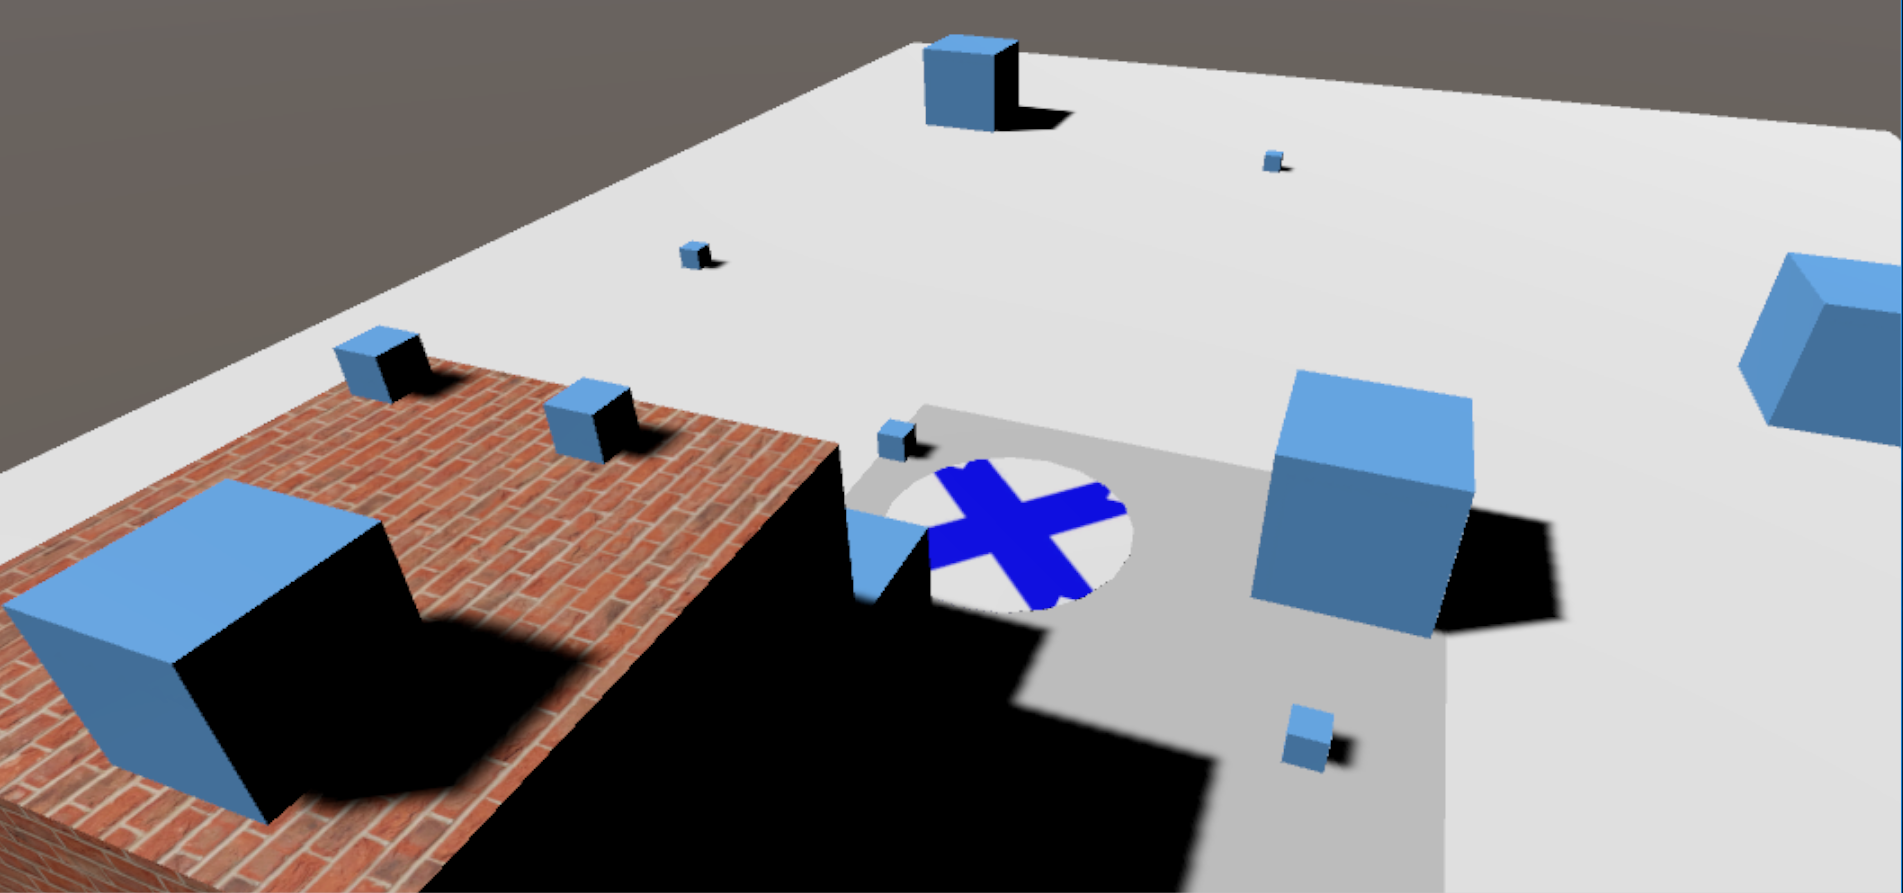
\includegraphics[width=12cm]{Images/learningRoom2.PNG}			
	\caption[Overview of the Learning Room.]{Overview of the Learning Room.}
	\label{fig:learning room}
\end{figure}

The room is designed very clean and simple. In different sizes and distances simple objects, in this case cubes, are distributed randomly. This is shown in figure \ref{fig:learning room}. The virtual room is slightly bigger than the usable room in reality. So the user is forced to user interactions, which are designed for larger distances, to move some objects (compare sections~\ref{sec:Raycast} and~\ref{sec:ExtendableRay}). Due to different colors of the floor the user know how big the real room is approximately. In addition the \textit{HTC Vive} system offers a coloured wire, which is shown in the HMD, whenever the user gets too close to the border of the calibrated area.\\
The user should already know the different interactions as well as the menu settings, when he enters the supermarket scene. So the menu and interactions are similar in both rooms. Also the labelling of the target object and the reaction of the target area to the target object will be established. This will be described in section~{sec:tasks}.\\ 
To get to know all settings and methods the user will be led to the entire learning room by a selfteaching system. This selfteaching is be described in section \ref{sec:selfteaching}. 


\subsubsection{Supermarket} \label{sec:supermarket} 
The second room is a small supermarket. 

\begin{figure}[H] 
	\center 
	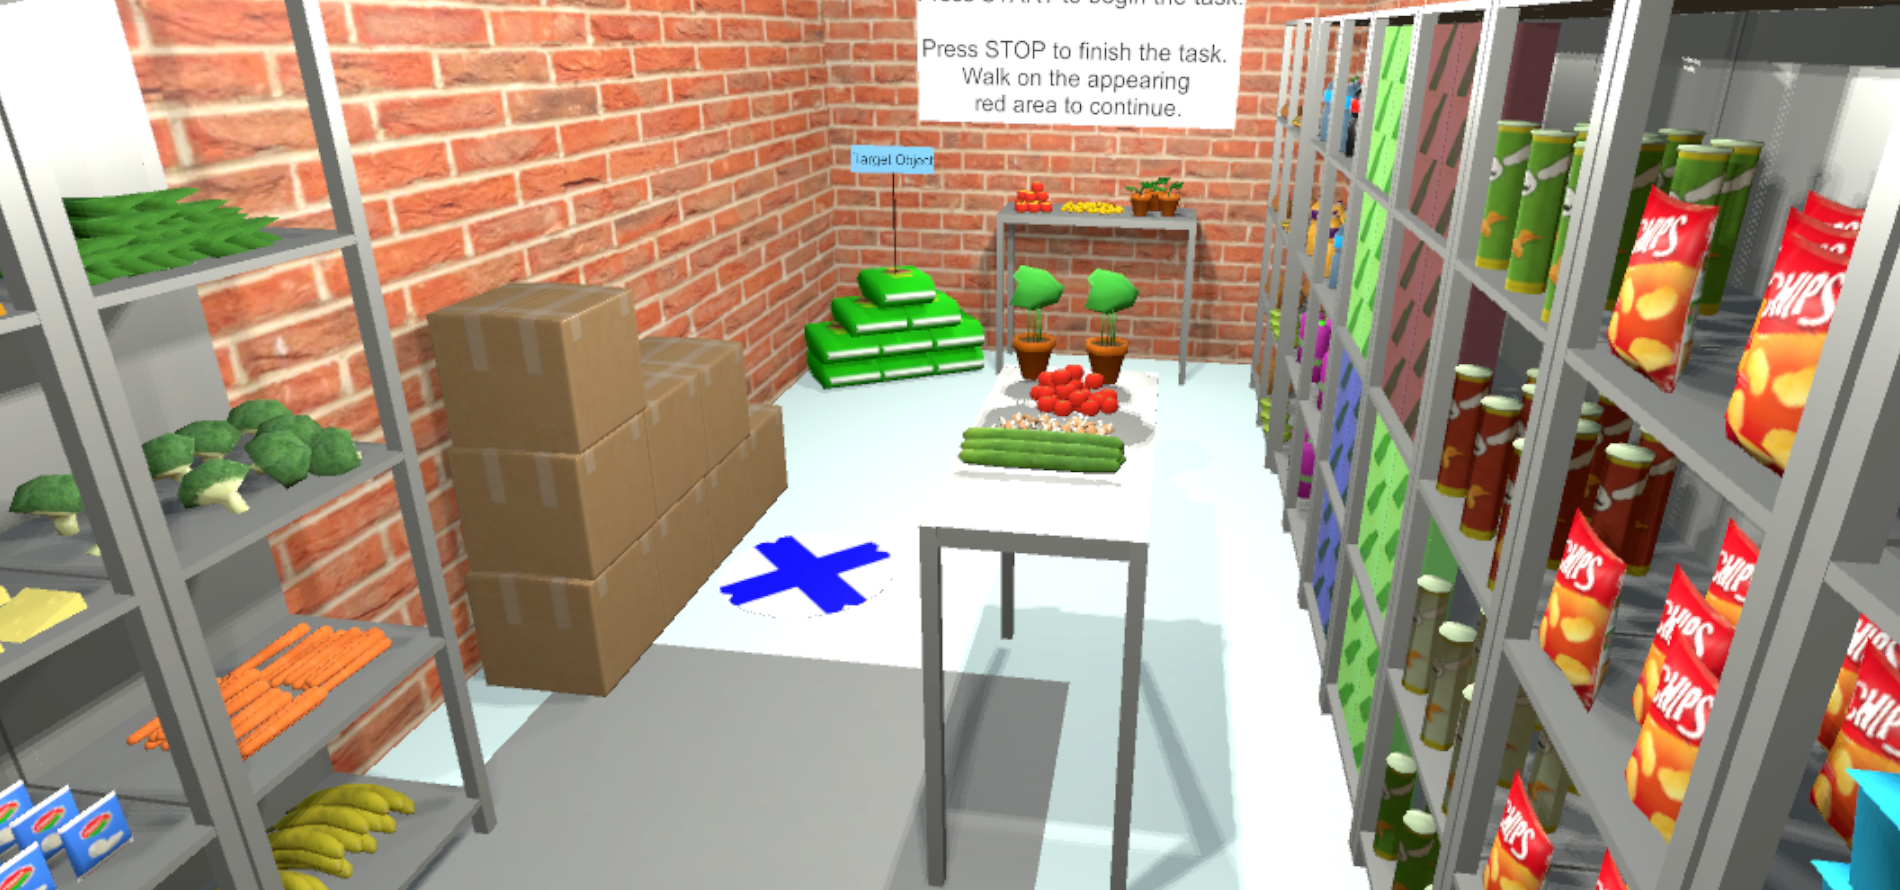
\includegraphics[width=12cm]{Images/supermarket.PNG}
	\caption[Overview of the supermarket.]{Overview of the supermarket.}
	\label{fig:supermarket}
\end{figure}

Like it is shown in figure \ref{fig:supermarket} in this supermarket are different sized objects in various distances. All objects could be found in a real supermarket, from fruits to milk. This objects were dowloaded from the asset store \cite{asset_food1} \cite{asset_food2} \cite{asset_box}. \\
The size of the real room is also displayed by using a slightly darker colour on the floor of the supermarket. This is necessary, because the supermarket is bigger than the real room. So interactions for far distance have to be used according to the tasks.

\begin{figure}[H] 
	\center 
	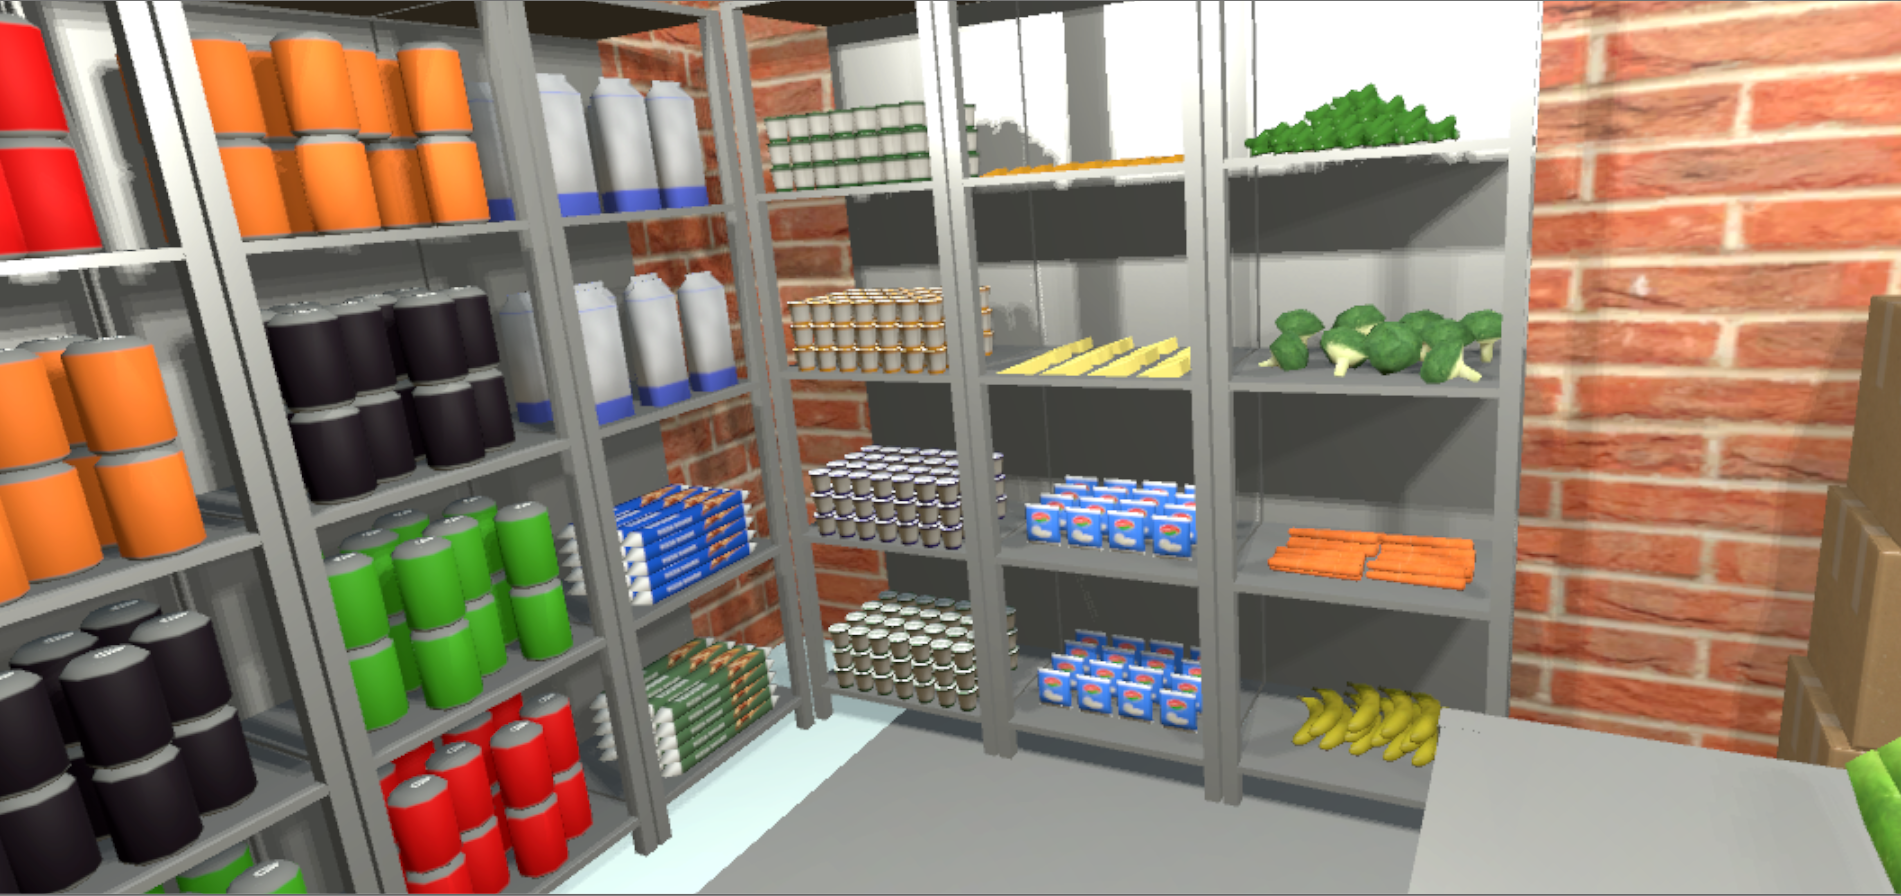
\includegraphics[width=12cm]{Images/supermarket2.PNG}
	\caption[Closer View of the Shelves.]{Closer view of the Shelves.}
	\label{fig:shelve}
\end{figure}

In some tasks the participant has to grab objects which are hard to pick. On one side they could be at a lower position, on the other side they could have to move other objects before they reach the labelled object. To implement this into a supermarket naturally shelves, like in figure \ref{fig:shelve}, are appropriate for a supermarket. This shelves were build with different scaled cubes.

\begin{figure}[H] 
	\center 
	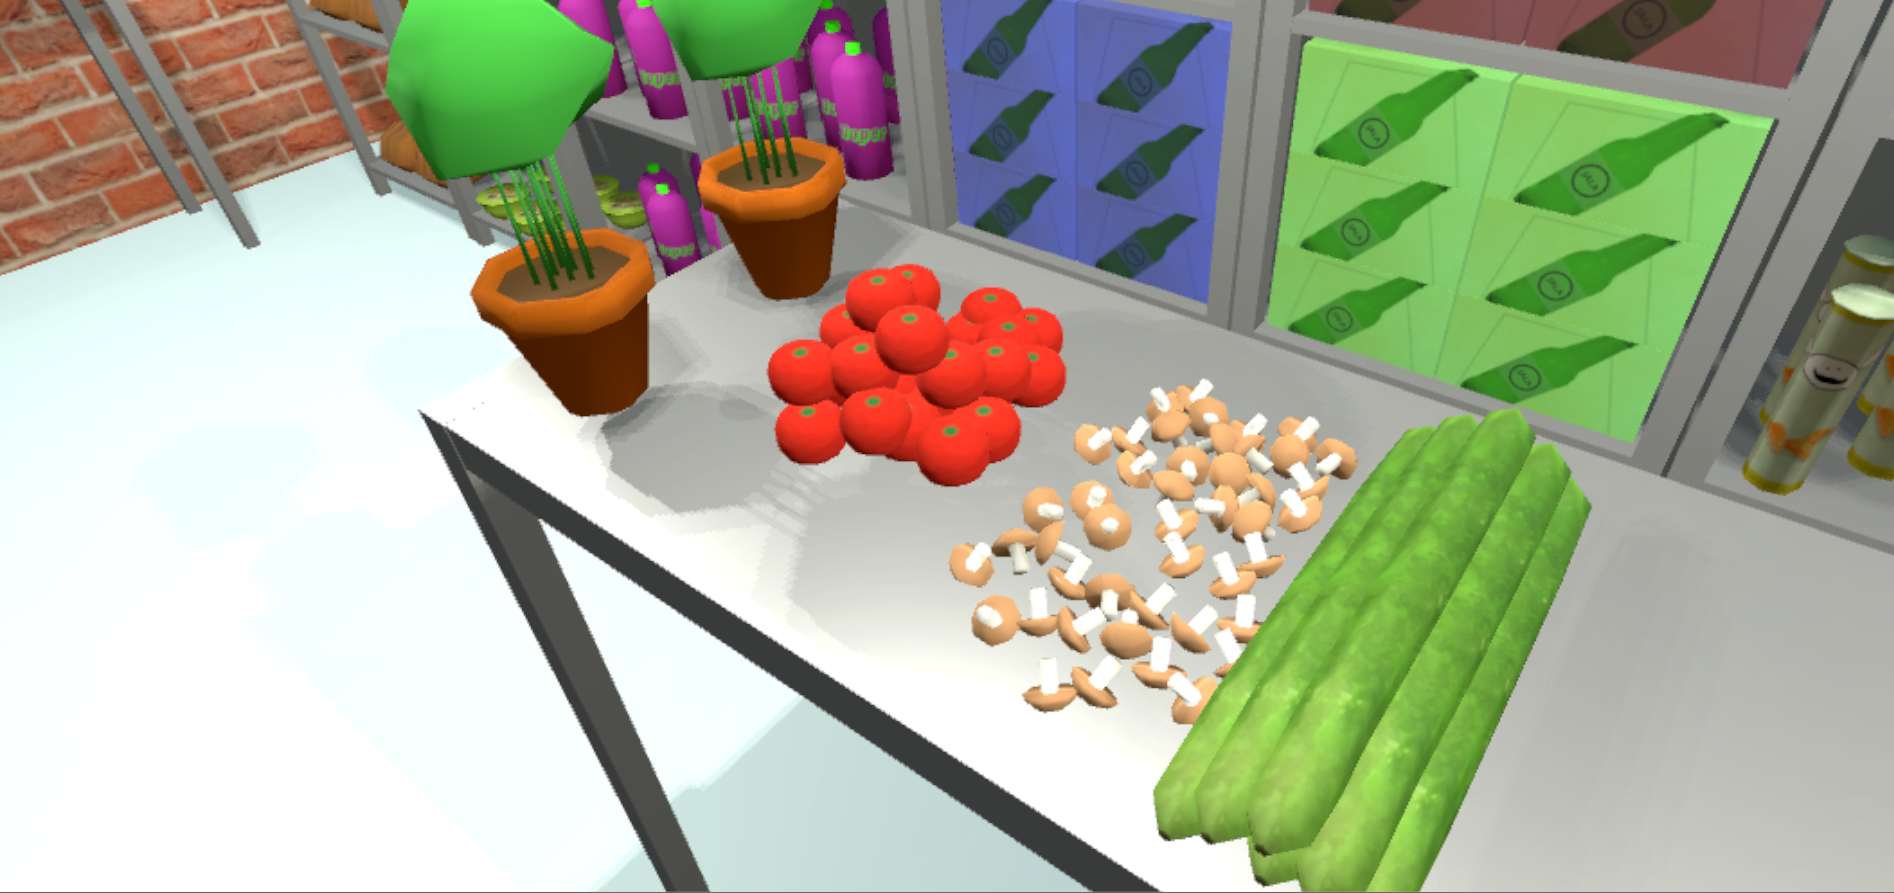
\includegraphics[width=12cm]{Images/supermarket1.PNG}
	\caption[Closer View of the Table.]{Closer View of the Table.}
	\label{fig:table}
\end{figure}	

In a real supermarket objects are not always arranged in shelves. Due to this fact and to have a variance for the tasks,  some objects where placed on tables as one bulk, for example fruits and vegetables. There are two tables in this supermarket. A closer look to one of this tables is given in figure \ref{fig:table}.\\
Depending on the task different target areas can appear in the supermarket. In this situations different objects will be blend out. Also the target object of every tasks will be labelled. The first target area and target object are shown in figure \ref{fig:supermarket}.\\
The structure of the labelling of the target object are specified in section \ref{sec:selfteaching}.
The different tasks as well as the reaction of the target area to the target object will be described in section \ref{sec:tasks}.

\subsection{Controller Menu} \label{sec:Menu}
%\todo[inline, color=red]{Anna}
The controller menu is the main menu of the system. It allows to change settings without leaving the virtual environment. Within this menu interaction methods can be changed and settings like snapping for the interactions can be enabled. In the learning room	the user is able to turn the selfteaching informations on and off. In the same way the user can decide if the tasks will be shown or not in the supermarket. In the supermarket scene the user can restart a single task via the controller menu. With the reset button the scene will be reloaded. The main menu is shown in figure~\ref{fig:mainMenu}.

\begin{figure}[H] 
	\center 
	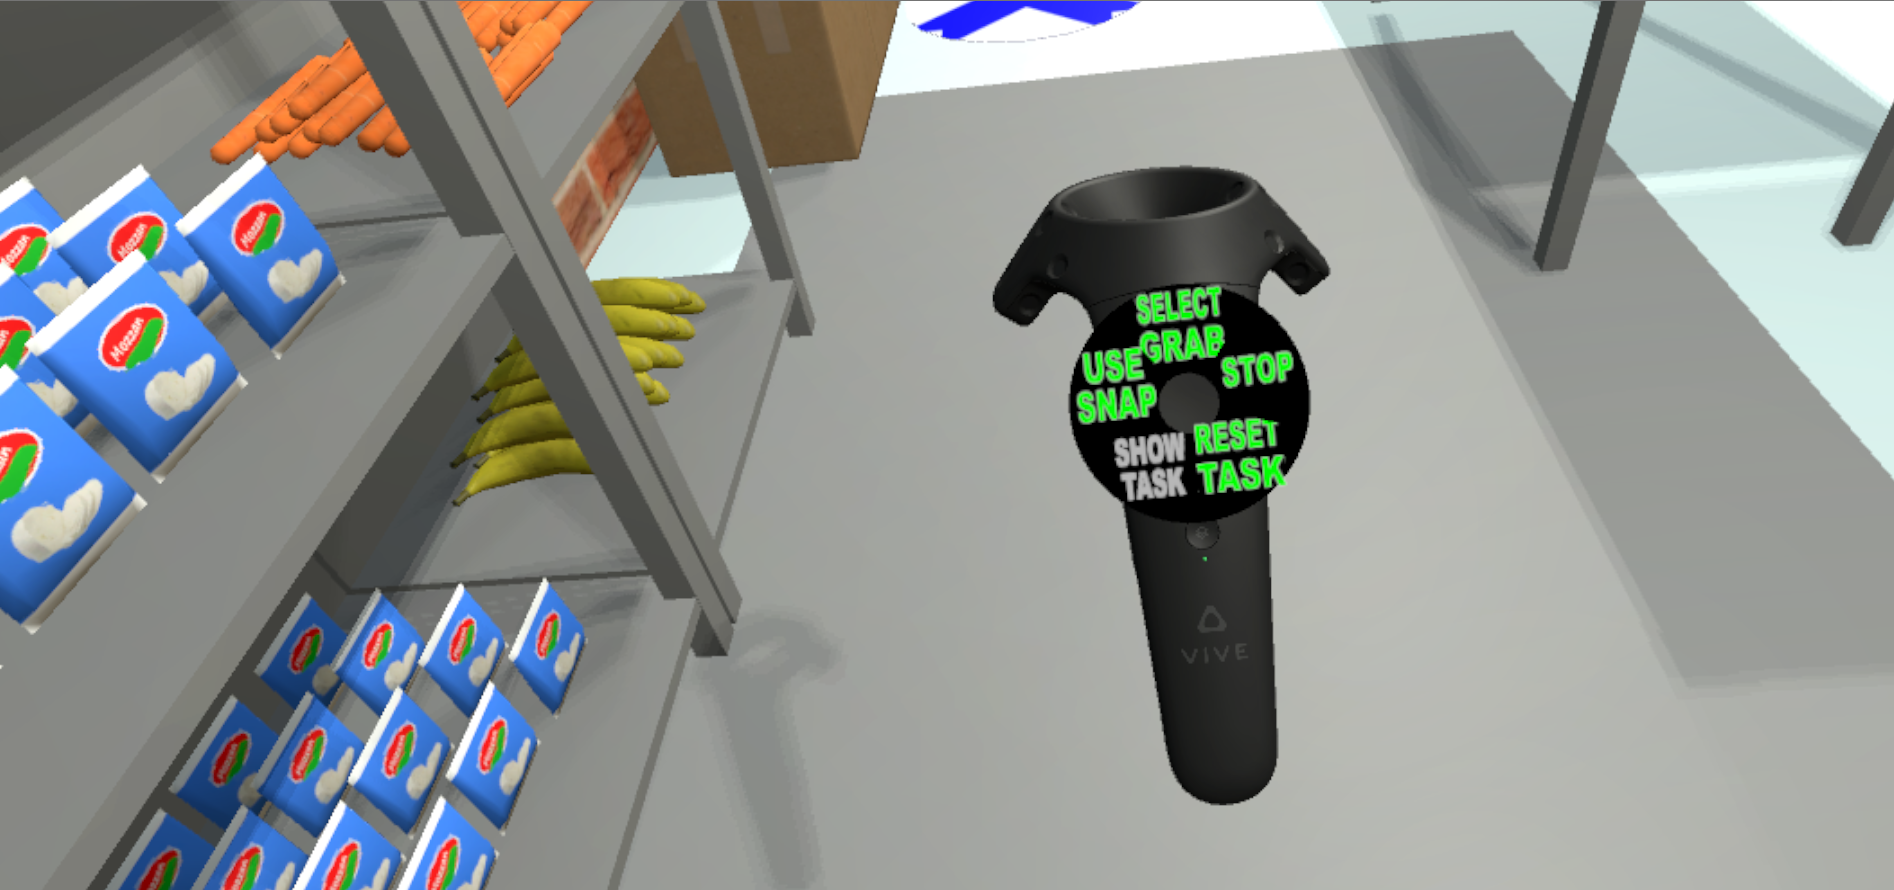
\includegraphics[width=12cm]{Images/Menu1.PNG}
	\caption[Main Menu of the Controller Menu.]{Main Menu of the Controller Menu.}
	\label{fig:mainMenu}
\end{figure}

If the button ``select grab'' is available, the user is able to choose every interaction method he likes. The button leads to an other menu. In this menu the methods are shown as icons, see figure \ref{fig:grabMenu}. The user learns the meaning of those icons with the help of the selfteaching, while they are in the learning room. 

\begin{figure}[H] 
	\center 
	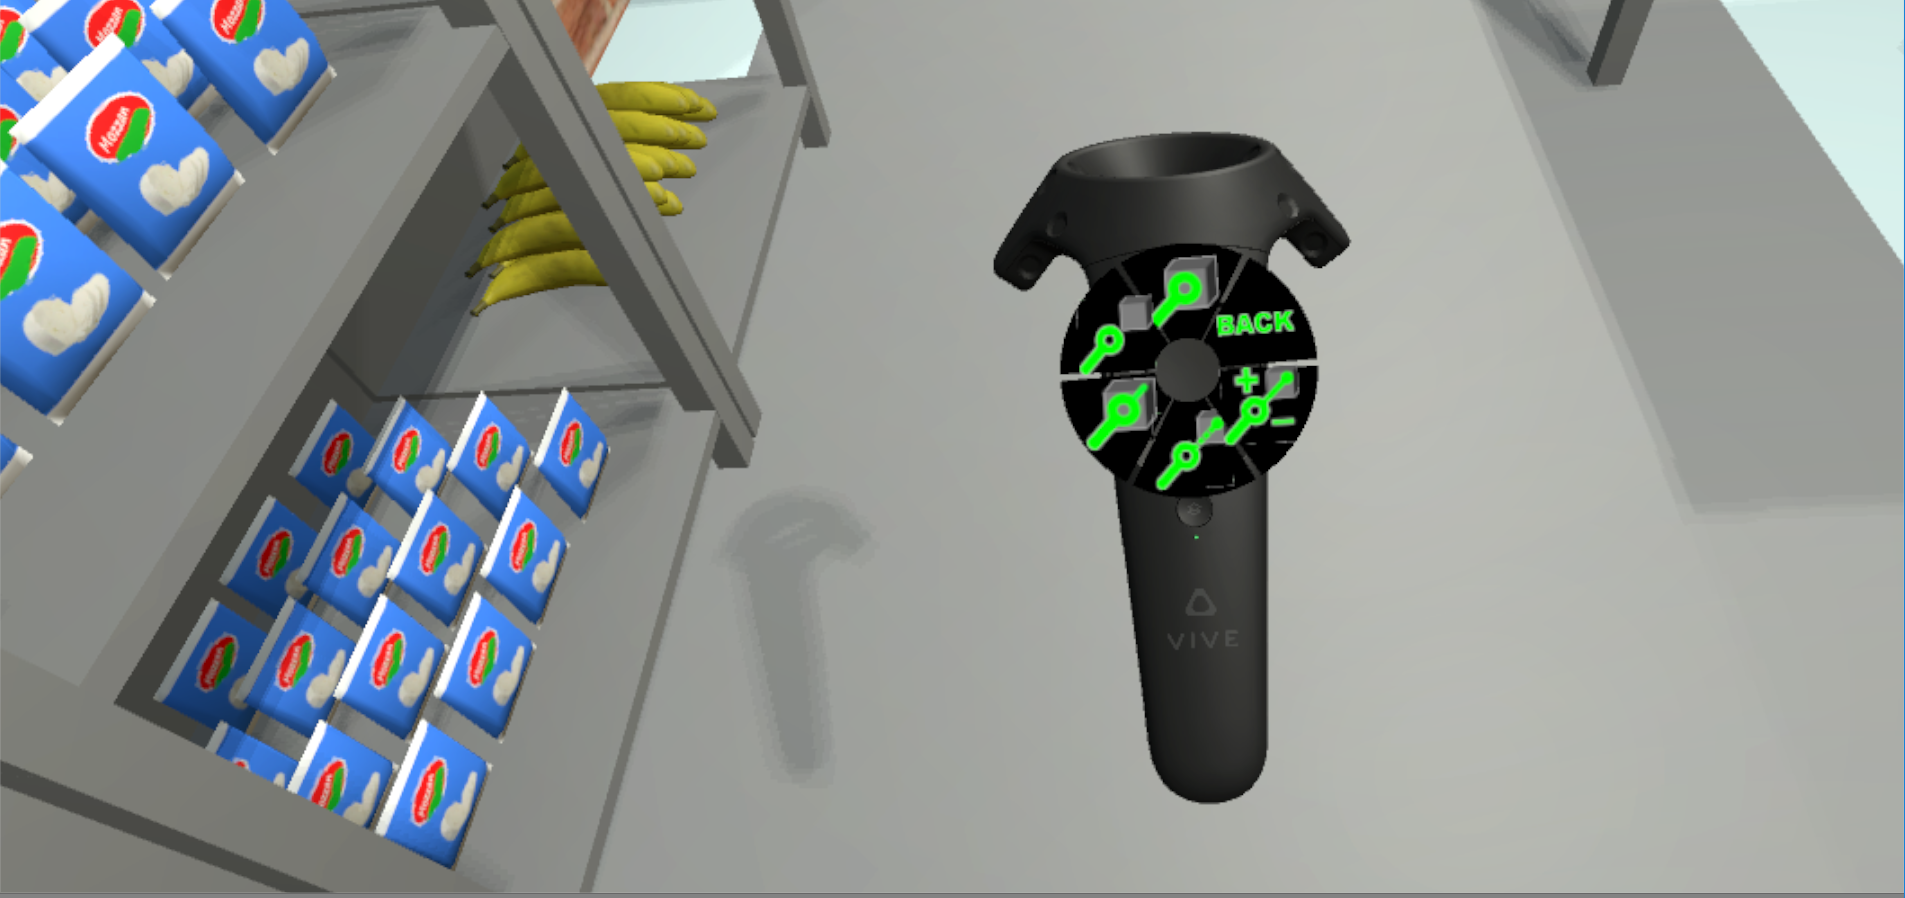
\includegraphics[width=12cm]{Images/Menu2.PNG}
	\caption[Select Grab Menu.]{Select Grab Menu.}
	\label{fig:grabMenu}
\end{figure}

For the measurement, which are described in section \ref{sec:measurement}, the user has to start and stop every tasks. The start button will be the first menu button in every scene. Only if this button is pressed the user can interact with the environment and will be led to the next menu. When the user presses the stop button the switching area will appear and the corresponding \textit{BoxCollider} \cite{website:BoxCollider} will be enabled. If the user reaches this area the next scene will be loaded.\\
The structure of the menu is built on the plug-in ``VRTK'' which is described in section \ref{sec:VRTK}.\\
In this project there is a script named \textit{Menu.cs} in which all functions for the menu are collected. Due to this script different settings can be chosen.


\subsection{Interaction Methods}\label{sec:Interactions}
Of course there were different interaction methods required to make the \textit{Interaction Lab} suitable for the testing described and evaluated in section~\ref{sec:evaluation}. Also all interaction methods are implemented to realise the grabbing of virtual objects, they can be separated in the two categories, described in the next two paragraphs:

\paragraph{Close Range (CR) Interactions:} The CR can be interpreted as a synonym for the natural interaction radius of the person. Due to this definition it is excluded that those interactions can be used outside an area, which the person can not reach with his arm, or to be more precise: with the controller in his hand. In other words: the CR combines all interactions which can be used to pick up objects in the direct reach of the user.

\paragraph{Far Range (FR) Interactions:} Due to a limitation of the range of motion in VR applications, it is common to have interactions designed for grabbing objects which are normally seen as out of the reach of the user~\cite{VRBook}. Interaction methods allowing such an acting are called FR interactions. It is not excluded, that a FR interaction is used in the actual reach of the user. \\

Whereas the CR interactions differ mainly in the accuracy of the selection of an object while grabbing it, the FR methods differ in their usability. All characteristics of the various interaction methods can be traced in their descriptions (compare sections~\ref{sec:TouchGrab} -~\ref{sec:RaycastHMD}).

For a better understanding it should be mentioned, that all interaction methods can be controlled with the \textit{HTC Vive}-controller. Even there are plenty of different possibilities to grab an object all methods have in common that the grabbing is caused by pressing the trigger on the \textit{HTC Vive}-controller. The releasing of the object is than triggered by letting it go. Whenever there is a divergent usability necessary, it is described in the respective section (compare~\ref{sec:ExtendableRay}).

Due to an easier integration into the learning room (compare section~\ref{sec:Learningroom}), as well as the actual supermarket scenes (compare section~\ref{sec:supermarket}) all methods using a ray (compare sections~\ref{sec:ExtendableRay},~\ref{sec:Raycast} and ~\ref{sec:WandGrab}) are summed up in one script called \textit{AllRaycastMethods.cs}. All other methods have their own script in which the grabbing and releasing is implemented. Also the \textit{Raycast Head Mounted Display}-method, described in section~\ref{sec:RaycastHMD}, is using a ray it is not included into the script mentioned above. This is caused by remaining problems during the implementation of this method which lead to an unfinished work. Further explanations on why this method is not available in the \textit{Interaction Lab} can be found in the according section.

The two interaction methods, described in sections~\ref{sec:TouchGrab} or rather~\ref{sec:ProximityGrab}, can be used with snapping or without it. This technique is used to reassign the position and orientation of a grabbed object in hand. By assuming that the middle of the ring of the \textit{HTC Vive}-controller is the new center of the grabbed object the actual grab could appear more realistic to the user. 

In the application all objects, which can be grabbed are tagged as moveable.\\

In the following sections all available interaction methods of the \textit{Interaction Lab} are presented. To guarantee a better overview they are sorted by their interaction range. 

\subsubsection{Close Range: Touch Grab} \label{sec:TouchGrab}
When the \textit{Touch Grab} interaction method is selected the user can make use of the \textit{HTC Vive}-controller to pick up objects directly by touching them. An object can be grabbed whenever it is tagged as moveable and collides with the \textit{HTC Vive}-controller. This collision is detected by giving the object a collider, which fits its form best \cite{website:BoxCollider}\cite{website:SphereCollider} and applying a \textit{BoxCollider} to the controller. The interaction can be seen in figure~\ref{fig:touchGrab}. \\
In the script \textit{TouchGrab.cs}, in which the interaction method is implemented, is checked frequently, whether there is a overlap of the collider of the controller with the collider of a moveable object or not. Whenever they collide, the respective object is coloured green to show the user that he could grab it by pulling the trigger. 

\begin{figure}[H] 
	\center 
	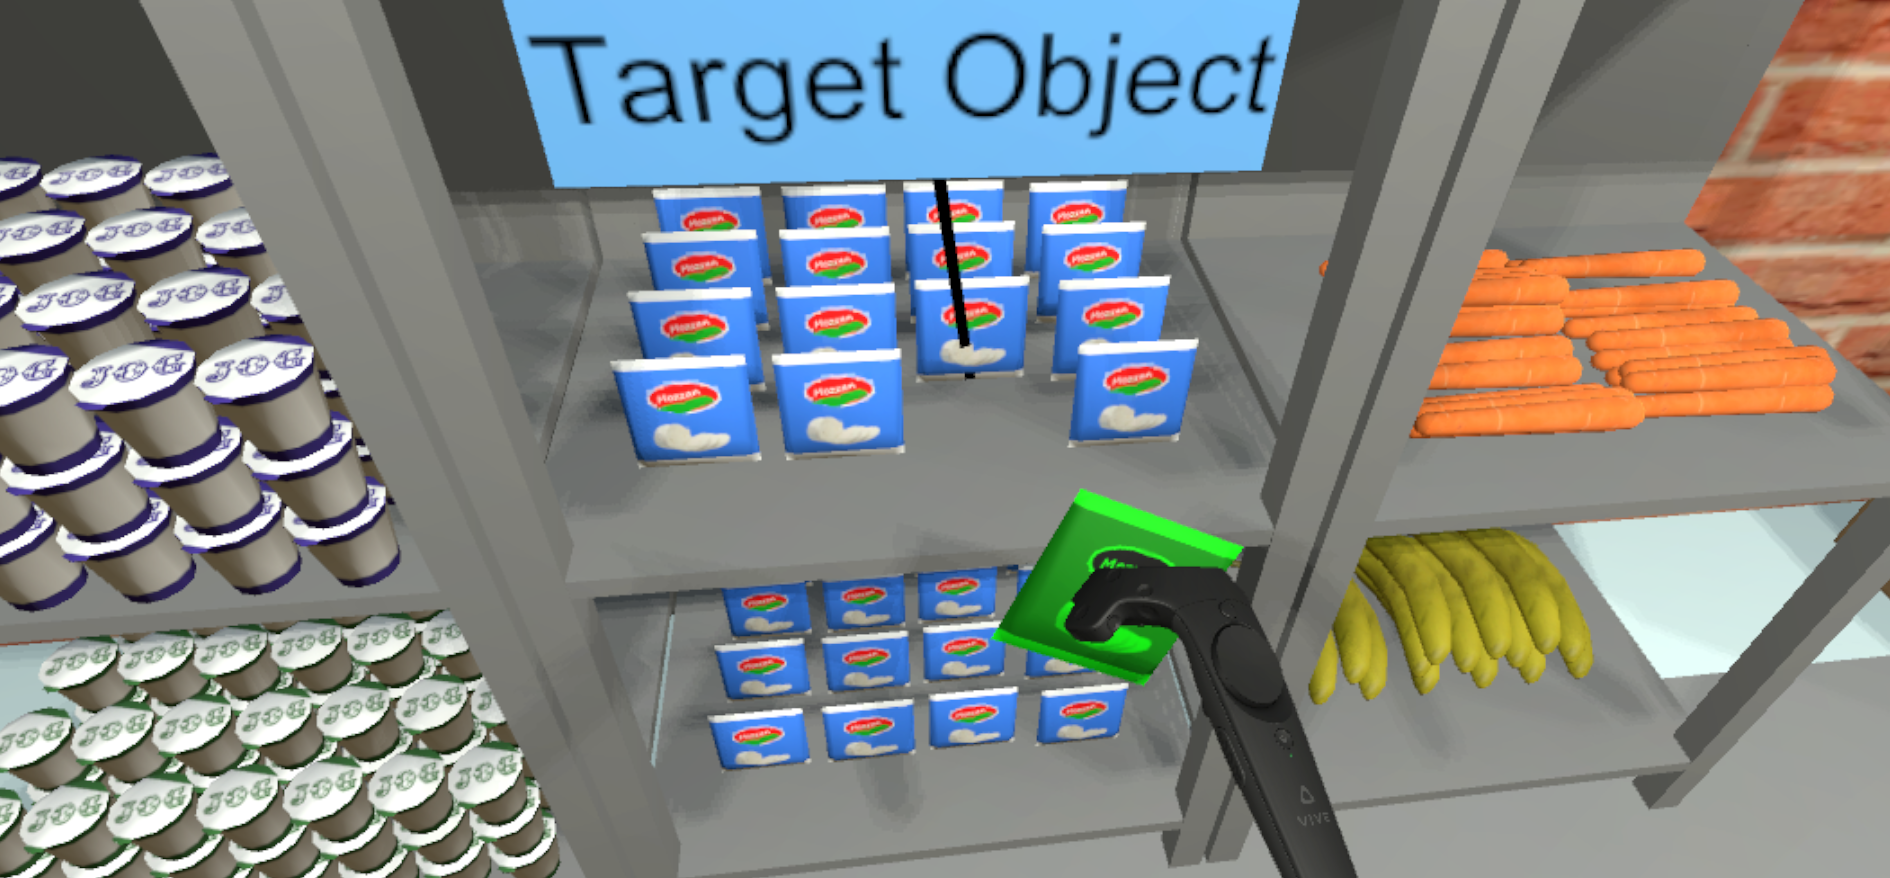
\includegraphics[width=12cm]{Images/TouchGrab.PNG}			
	\caption[Grabbing a virtual object by using \textit{Touch Grab}.]{Grabbing a virtual object by using \textit{Touch Grab}.}
	\label{fig:touchGrab}
\end{figure}

\subsubsection{Close Range: Proximity Grab} \label{sec:ProximityGrab}
When it comes to the CR interactions the \textit{Proximity Grab} is by far the most inexact selection.  \\
The functionality is provided by the script \textit{ProximityGrab.cs}. The basic idea is that the object can be grabbed, whenever the object triggers the \textit{BoxCollider} \cite{website:BoxCollider} placed at the end of the \textit{HTC Vive}-controller. A more detailed description can be found in section \ref{sec:TouchGrab}. In contrast to the \textit{Touch Grab} described in section~\ref{sec:TouchGrab} this \textit{BoxCollider} is bigger than the actual size of the controller. To show the user, which object collides with the controller and can therefore be grabbed, the respective object is coloured green, as shown in figure~\ref{fig:proximityGrab}. The small gap between the actual grabbed object and the controller shows the difference between the interaction method shown in figure~\ref{fig:touchGrab}.

\begin{figure}[H] 
	\center 
	\includegraphics[width=12cm]{Images/ProximityGrab.PNG}			
	\caption[Grabbing a virtual object by using \textit{Proximity Grab}.]{Grabbing a virtual object by using \textit{Proximity Grab}.}
	\label{fig:proximityGrab}
\end{figure}


\subsubsection{Close Range: Wand Grab} \label{sec:WandGrab}
In contrast to the interaction method described in \ref{sec:ProximityGrab} this method can be used to grab very tiny objects. Thereby it is not needed that the target object is very isolated from other objects. To give the user such an high grade of accuracy a stick is added to the controller like shown on figure~\ref{fig:wandGrab}. \\
The implementation can be found in \textit{AllRaycastMethods.cs}. The wand consists of two elements: a ray \cite{website:Ray} and a cube. The cube is only for the visualisation and has a fixed size in all three dimensions. The collision detection, which is necessary for the actual grabbing, is done with the ray. That means that an object can be grabbed if the ray, which has the same dimensions like the cube, touches this specific object. The stick will then turn from black to green to show the user that there is an object which can be grabbed.

\begin{figure}[H] 
	\center 
	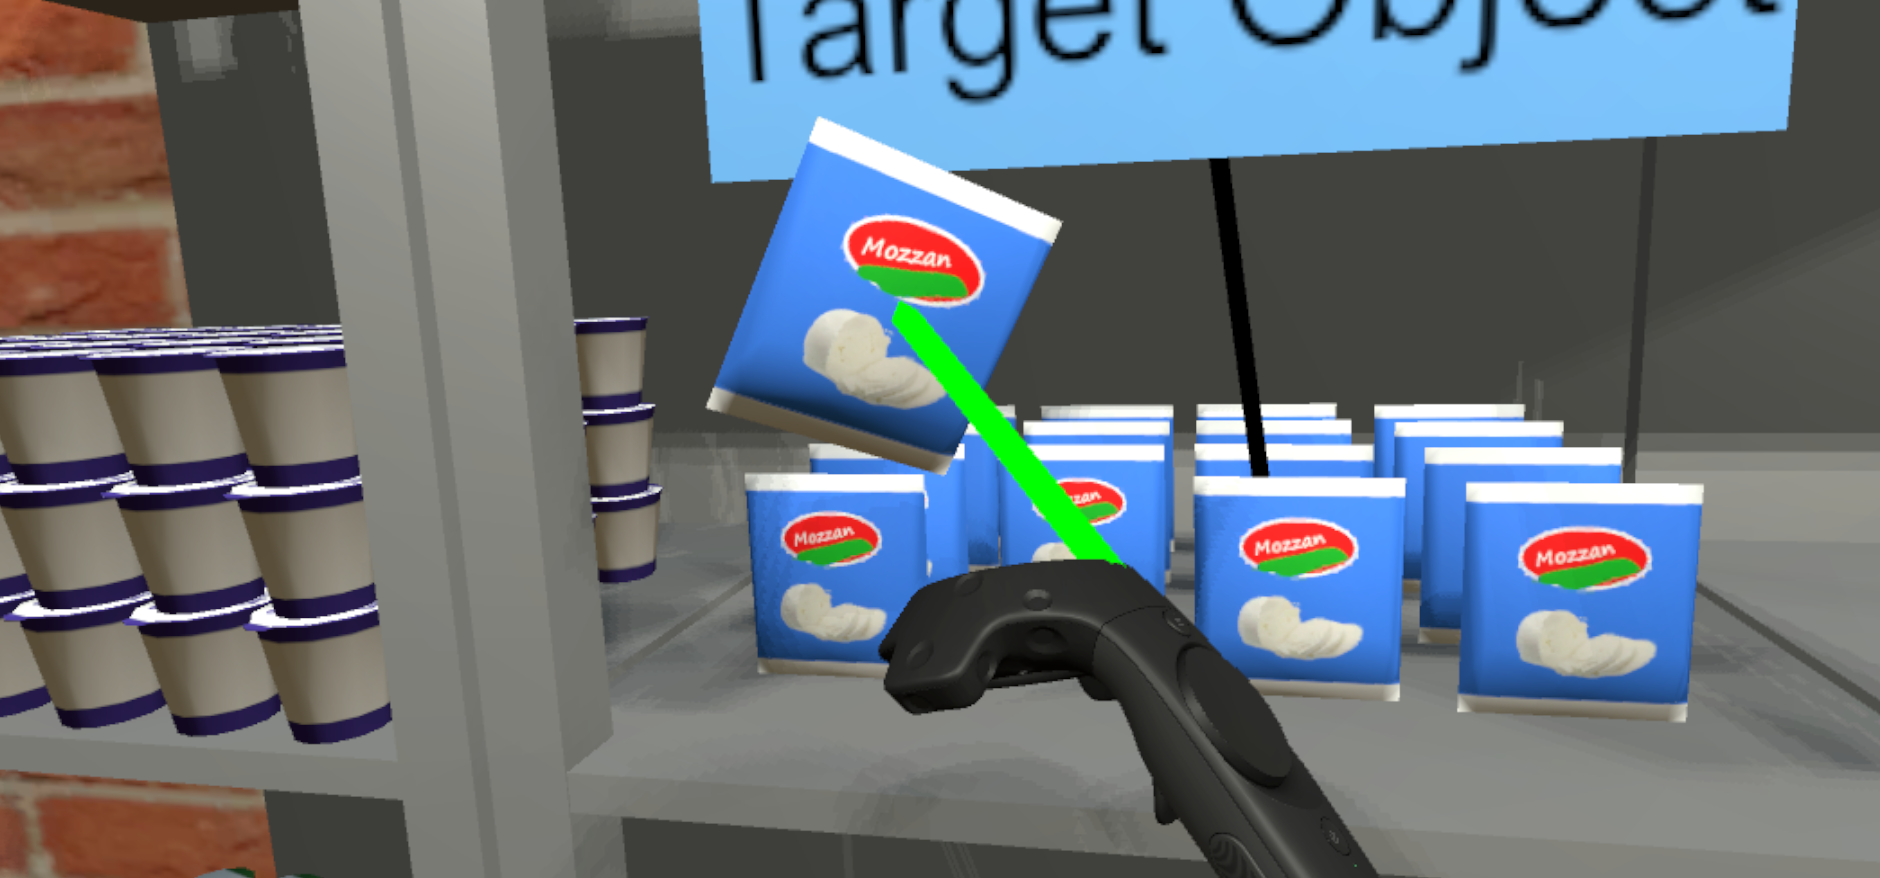
\includegraphics[width=12cm]{Images/WandGrab.PNG}			
	\caption[Grabbing a virtual object by using \textit{Wand Grab}.]{Grabbing a virtual object by using \textit{Wand Grab}.}
	\label{fig:wandGrab}
\end{figure}

\subsubsection{Far Range: Raycast} \label{sec:Raycast}
By using the \textit{Raycast} method the user can grab virtual objects which are further away as well as objects in his CR. As shown in figure~\ref{fig:raycast} a ray is coming out of the \textit{HTC Vive}-controller pointing away from the user. At the end of the ray is a small sphere, which turns green, if it collides with an moveable object. Whenever the ray hits an objects, like for example the floor or a product in the supermarket (compare section~\ref{sec:supermarket}), the ray is shortened to the distance between the controller and the respective object. \\
The implementation can be found in the \textit{AllRaycastMethods.cs} script. As already explained in section \ref{sec:WandGrab} a cube and a ray are combined to reach the intended functionality. In contrast to the \textit{Wand Grab}, the ray and the visible cube have no fixed length and there is a sphere added to the end of the cube.

\begin{figure}[H] 
	\center 
	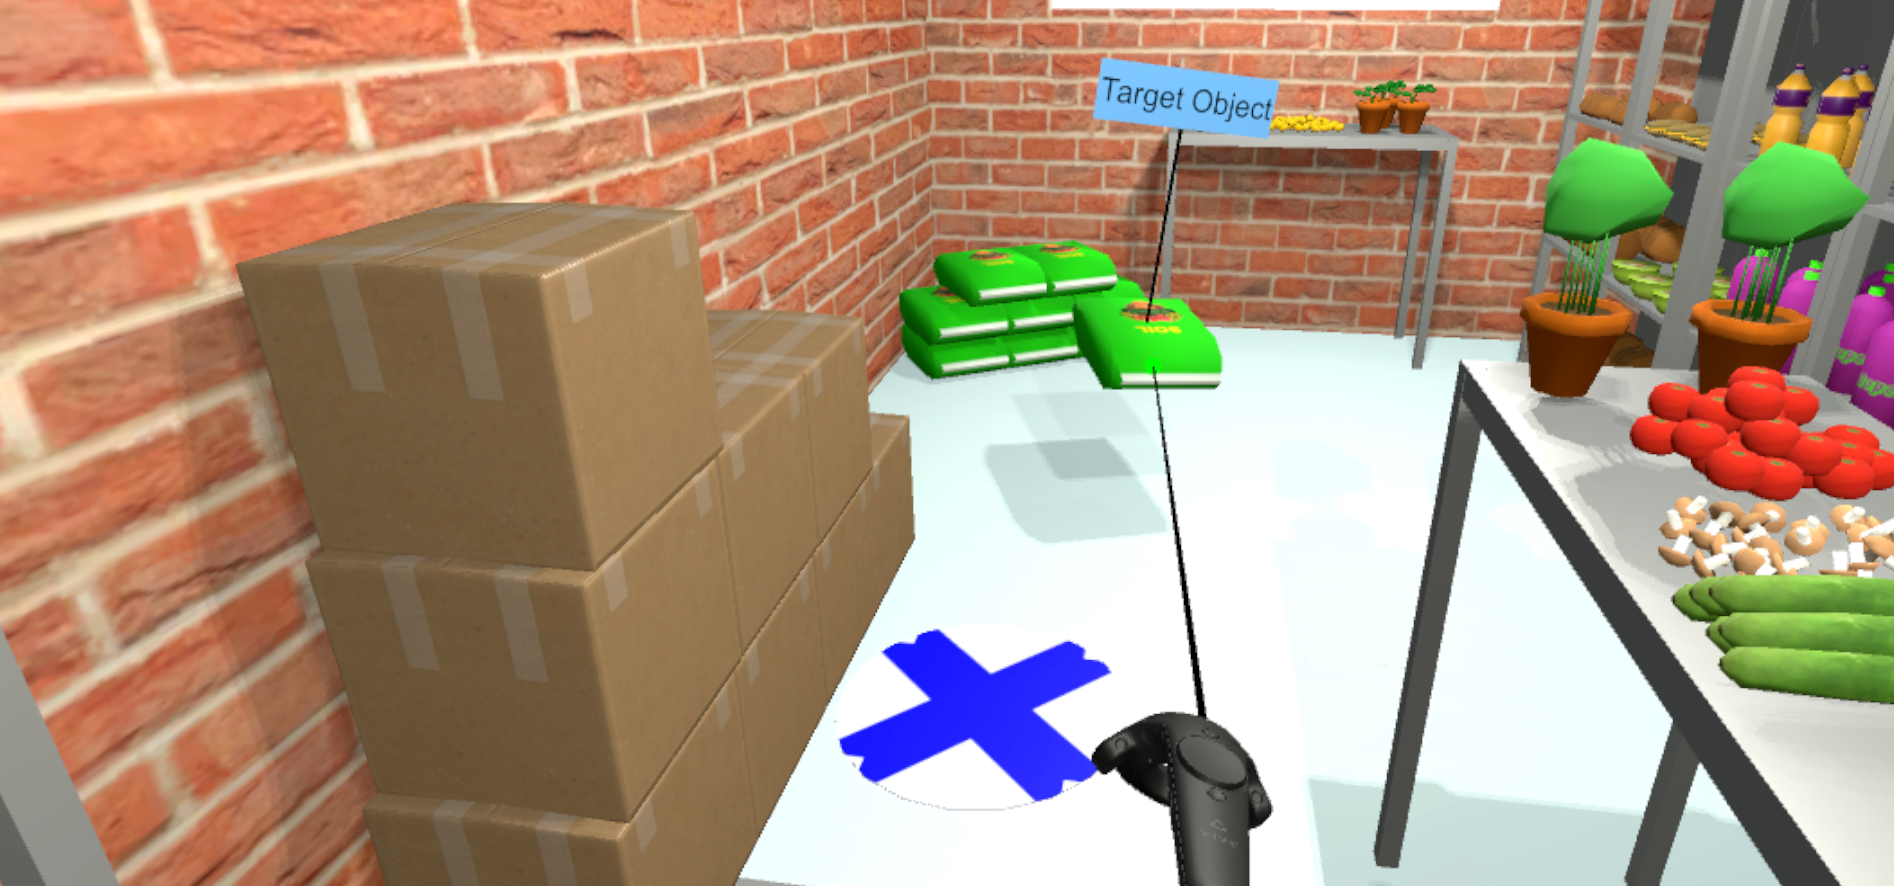
\includegraphics[width=12cm]{Images/Raycast.PNG}			
	\caption[Grabbing a virtual object by using \textit{Raycast}.]{Grabbing a virtual object by using \textit{Raycast}.}
	\label{fig:raycast}
\end{figure}


\subsubsection{Far Range: Extendable Ray} \label{sec:ExtendableRay}
The actual ray is build as described in section \ref{sec:Raycast}. The ray \cite{website:Ray} is complemented by a cube with a sphere at the end, to make it visible for the user. In contrast to the normal \textit{Raycast} method the length of the ray is set to a start value of 3 meters. The user can shorten and lengthen the ray by pressing the touchpad of the \textit{HTC Vive}-controller in the lower or rather upper area. This subtracts or adds a constant value to the length of the visible ray. The behaviour of the sphere remains, which turns green, whenever a moveable virtual object is brushed. The \textit{Extendable Ray} is one of the three interactions methods (compare sections~\ref{sec:WandGrab} and~\ref{sec:Raycast}) which are combined in the \textit{AllRaycastMethods.cs} script. This interaction method is shown on figure~\ref{sec:ExtendableRay}.

\begin{figure}[H] 
	\center 
	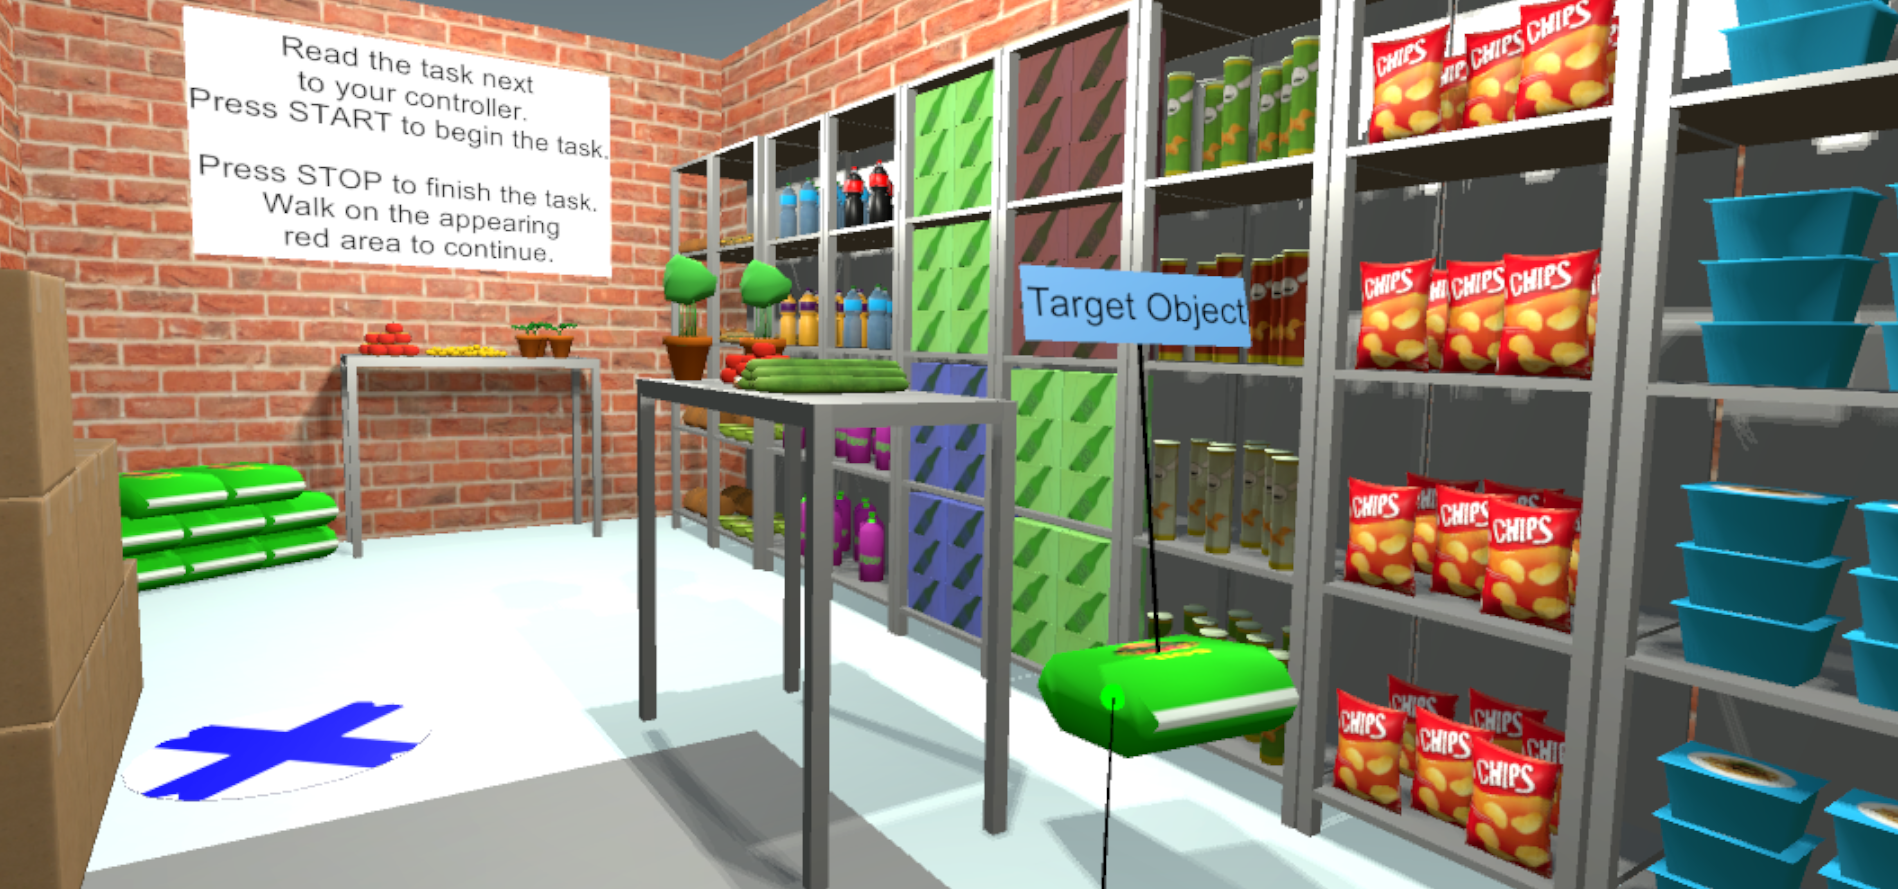
\includegraphics[width=12cm]{Images/ExtendableRay.PNG}			
	\caption[Grabbing a virtual Object by using \textit{Extendable Ray}.]{Grabbing a virtual Object by using \textit{Extendable Ray}.}
	\label{fig:extendableRay}
\end{figure} 


\subsubsection{Far Range: Raycast Head Mounted Display} \label{sec:RaycastHMD}
It was planned to realise an interaction method where there is a ray coming out of the HMD which can be used similar to the method described in section~\ref{sec:Raycast}. Due to the low accuracy of this method it did not become a part of the \textit{Interaction Lab}. There was a try to parent \cite{website:SetParent} the position of the HMD to the starting point of the ray. It turned out that the parenting-method is not successful when it comes to the position and rotation of the HMD. Even this method was effective for adding a ray to the \textit{HTC Vive}-controller, there is a irregular shift when you try to implement it with the HMD. To proof that an easy example (compare source code~\ref{lst:testHMD}) was observed. In this example a simple cube should be rendered at the front of the HMD. In reality this cube was rendered in a position which can be seen as random. 

\lstinputlisting[title=\lstname, caption={Test on the parenting of \textit{HTC Vive}-HMD and an virtual object.}, label=lst:testHMD, language={[Sharp]C}, linerange=1, firstnumber=1]{SourceCode/HMDtest.cs} 

All effort on this method can be found in the script \textit{RaycastingMethodeHMD.cs}.


\subsection{Self-Teaching} \label{sec:selfteaching}
\todo[inline, color=red]{Anna}
To guarantee an easy and smooth introduction to the system, an automatic selfteaching is integrated into the learning room. When the program is started all necessary instructions will be shown next to the controller, like shown in figure~\ref{fig:teaching1}. 

\begin{figure}[H] 
	\center 
	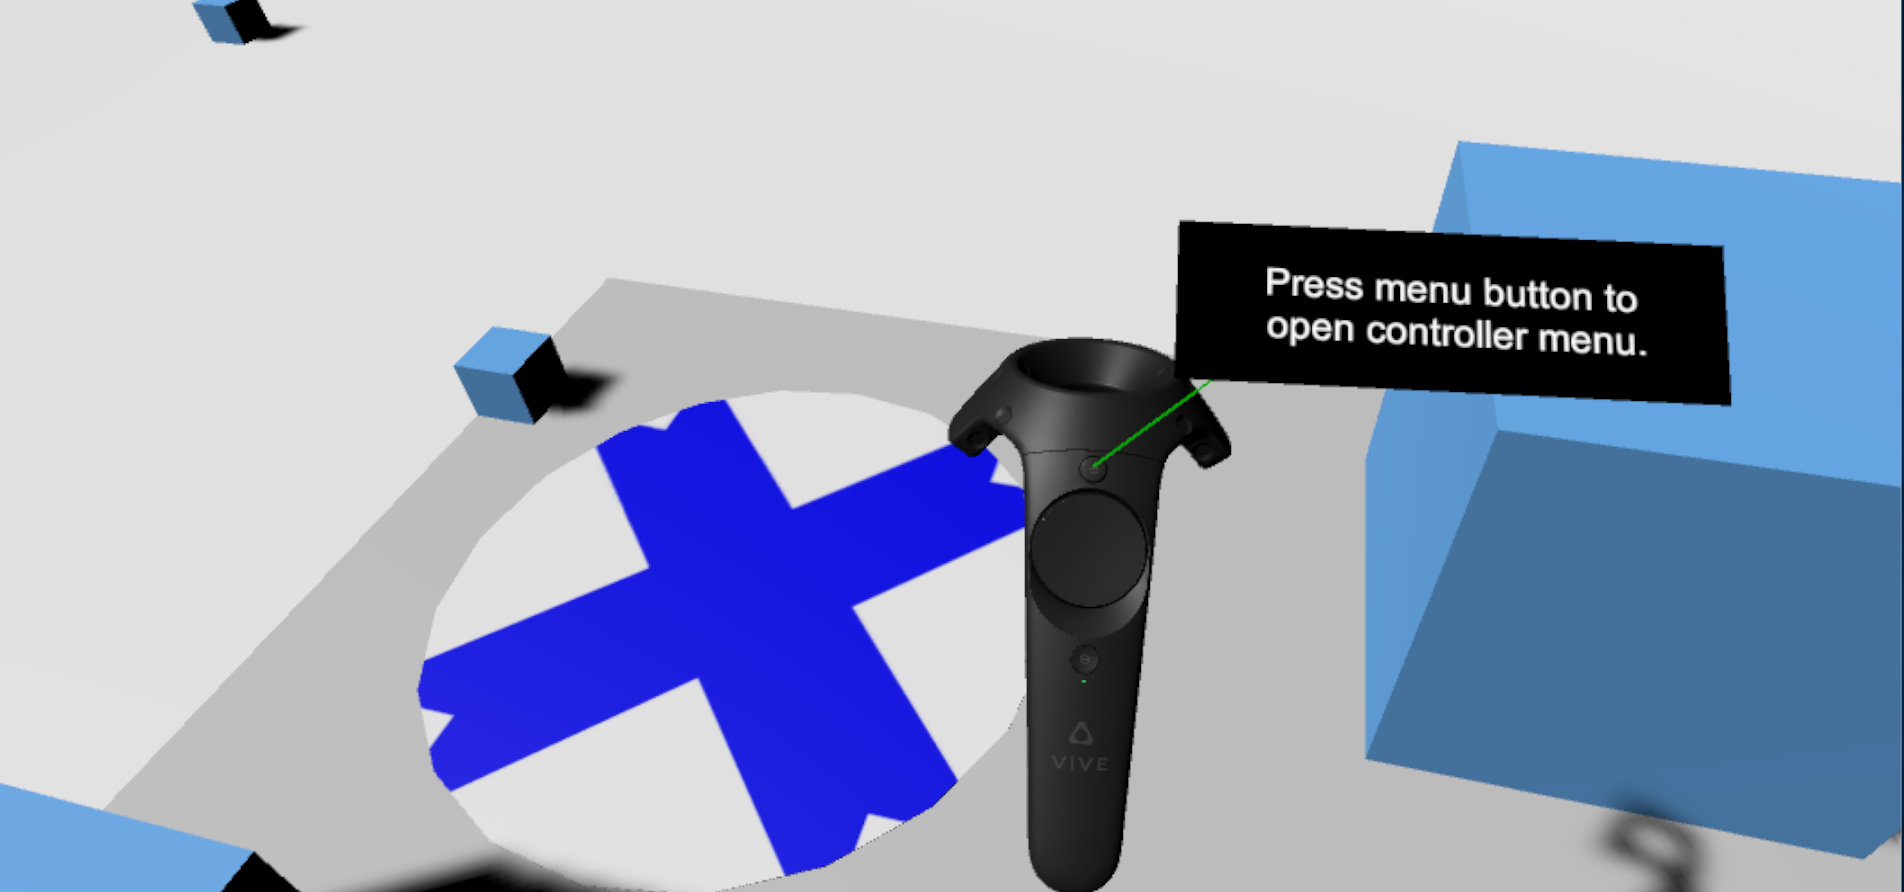
\includegraphics[width=12cm]{Images/teaching.PNG}
	\caption[Start of the Selfteaching.]{Start of the Selfteaching.}
	\label{fig:teaching1}
\end{figure}

This instructions led the user step by step through the system. He will get to know how the interaction methods can be chosen and what settings can be made. Of course the actual grabbing and releasing of an object is taught as well, for every interaction method. 

\begin{figure}[H] 
	\center 
	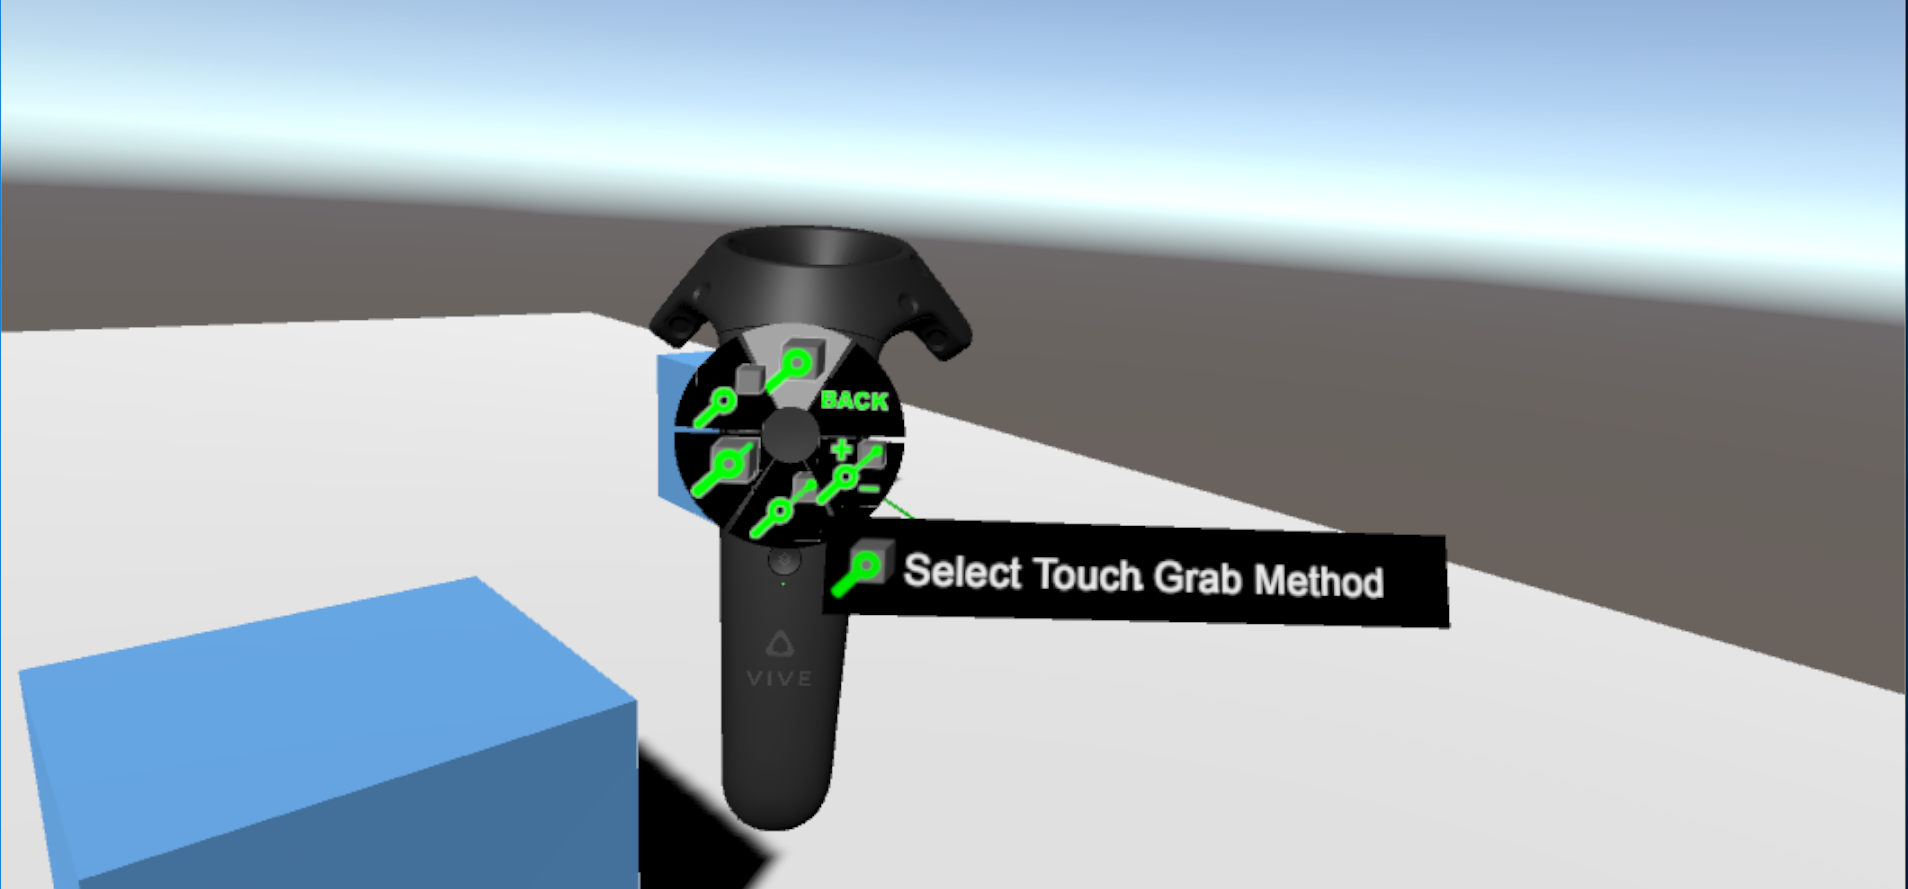
\includegraphics[width=12cm]{Images/teaching2.PNG}
	\caption[Selfteaching recommends to select \textit{Touch Grab} method.]{Selfteaching recommends to select\textit{Touch Grab} method.}
	\label{fig:teaching2}
\end{figure}

The instructions will only be visible in the learning room. The position of the information area changes depending on which button is important for the interaction. \\
In the first grab method, the \textit{Touch Grab} method, two terms will be established, which are important for all tasks. This terms are the labelling of the target object and the target area. Here the user learns how the target object is marked, compare figure \ref{fig:teaching3}, and how the target area reacts to the target object.

\begin{figure}[H] 
	\center 
	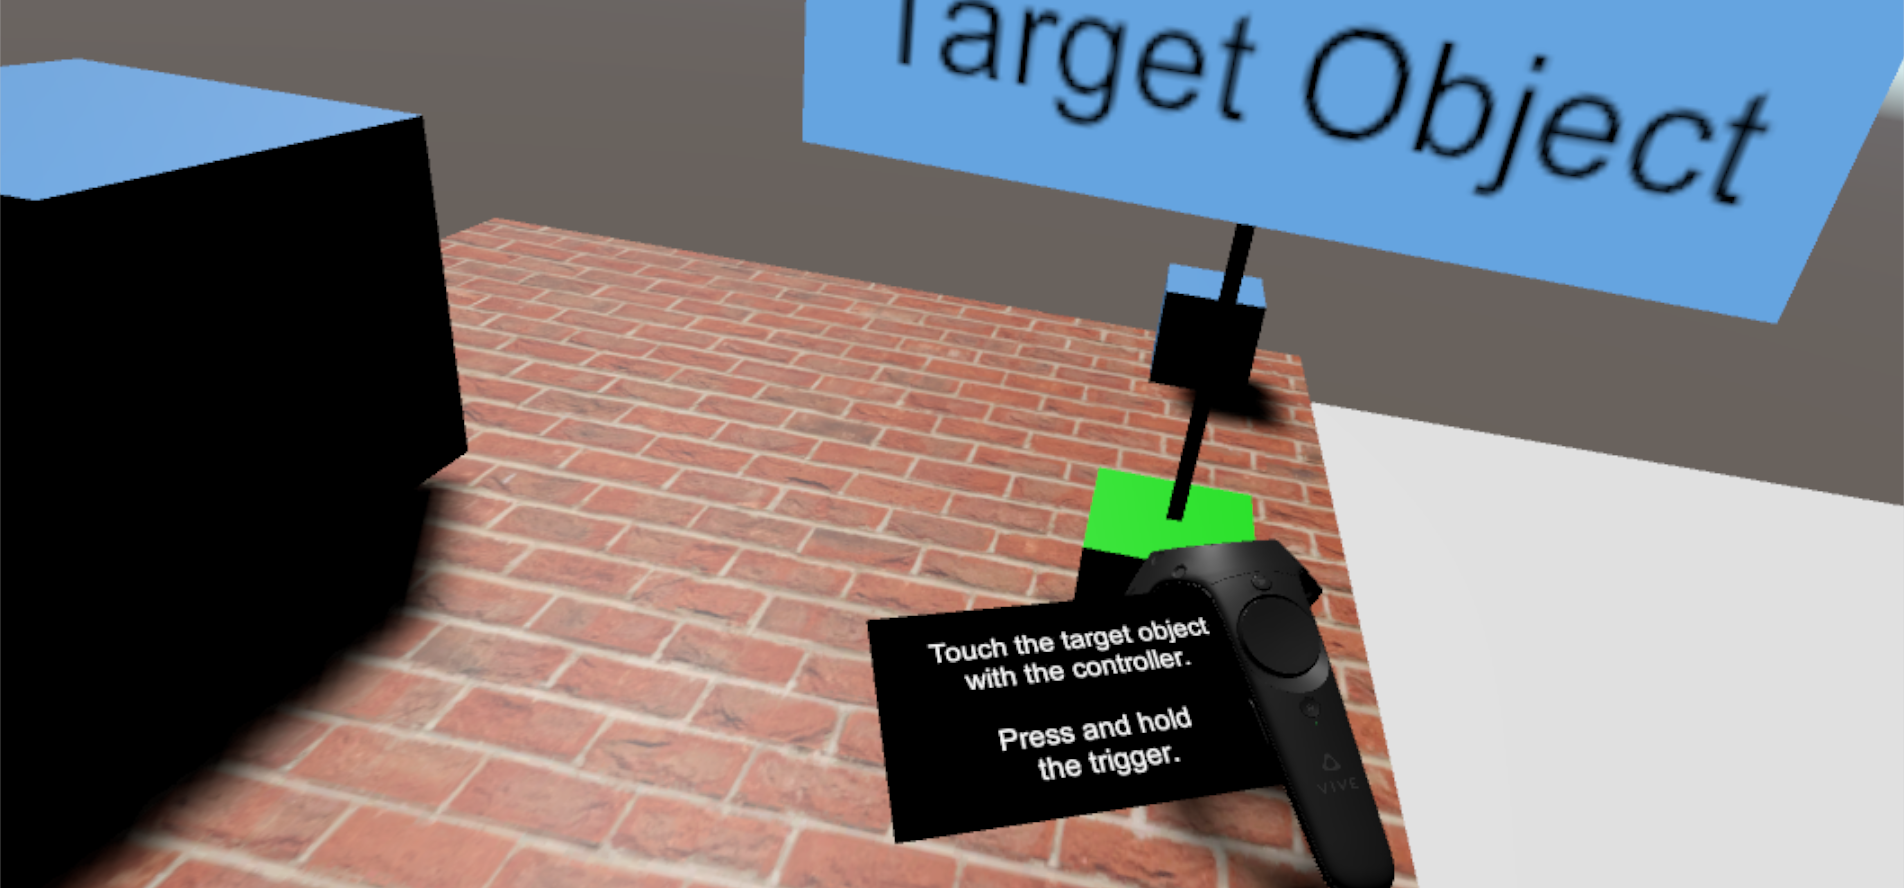
\includegraphics[width=12cm]{Images/teaching3.PNG}
	\caption[Selfteaching with Target Object.]{Selfteaching with Target Object.}
	\label{fig:teaching3}
\end{figure}

All instructions and steps of the selfteaching are saved in an external CSV-file, see following figure. 

\begin{figure}[H] 
	\center 
	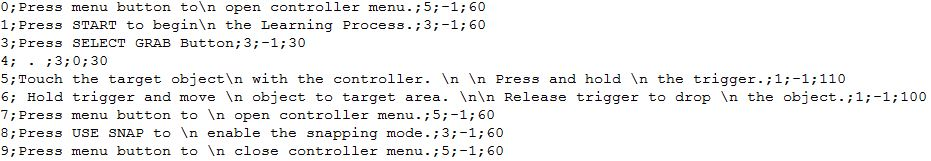
\includegraphics[width=15cm]{Images/selfteachingCSV.JPG}
	\caption[Extract of the CSV-file of the instructions of the selfteaching.]{Extract of the CSV-file of the instructions of the selfteaching.}
	\label{fig:teachingCSV}
\end{figure}

Due to an additional script \textit{WriteMeasureFile.cs} this file will be read line after line and be saved into different lists. In each line are four main information. The first number has no effect any more. The first important information is the text which should be shown in this step. Second is the Button ID, which defines on which button the information should be fixed. Third is a number which characterises if a material should be loaded.\textcolor{red}{Vielleicht hier die Nummerierung nach den Spalten machen also stringent von 1-4? Auch wenn die erste Zahl nicht mehr notwenig ist?} If this number is a $-1$, no material will be loaded and the text will be displayed on its own. If this number equals $0$ a specific material will be loaded into the canvas. Which material will be loaded is defined in the \textit{SelfTeaching.cs }script. The fourth \textcolor{red}{When ja dann hier fifth :)}and last information of the CSV-file is the height of the information area. This height changes depending on the amount of information. For each of this information a list is implemented in the \textit{SelfTeaching.cs} script.\\
In this script a counter is implemented. This counter controls which line of the file will be displayed. It will be increased or set from different scripts depending on an action. This increasing is still a problem, if the user does not follow the instructions of the selfteaching step by step. For example, if the user grabs an object twice and the selfteaching plans to grab it just once, the selfteaching will go on and the user misses instructions. \\
The instruction canvas is established by the \textit{controller tips} prefab of the ``VRTK'' plug-in, see section \ref{sec:VRTK}. This plug-in has also a prefab for \textit{object tips}. With this prefab the target objects are labelled.


\newpage
\section{Evaluation} \label{sec:evaluation}
\textcolor{red}{Hier fehlt die Einführung, Britta}

\subsection{Tasks} \label{sec:tasks}
The supermarket (compare section~\ref{sec:supermarket}) is confronted with four tasks. In every task, an object has to be selected and placed on a target area. If the correct object is placed, the target area will change the color to signal that the tasks is successful done. In the script \textit{TargetTest.cs}, which is added as a component to the target object, is recognized when the target object hits the target area. At this moment the texture of target area is changed and the measurement (compare section~\ref{sec:measurement}) is stopped. \\
In the first three tasks the user has to select different objects. Therefore the user can decide which method he/she uses to grab the object. The selected method should differ depending on the tasks. In these tasks objects far away as well as in the CR should be picked. \\
The tasks will be shown next to the controller similar to the selfteaching (compare section~\ref{sec:selfteaching}), which the user is already aware of. The placement of the tasks is shown in the following figure. 

\begin{figure}[H] 
	\center 
	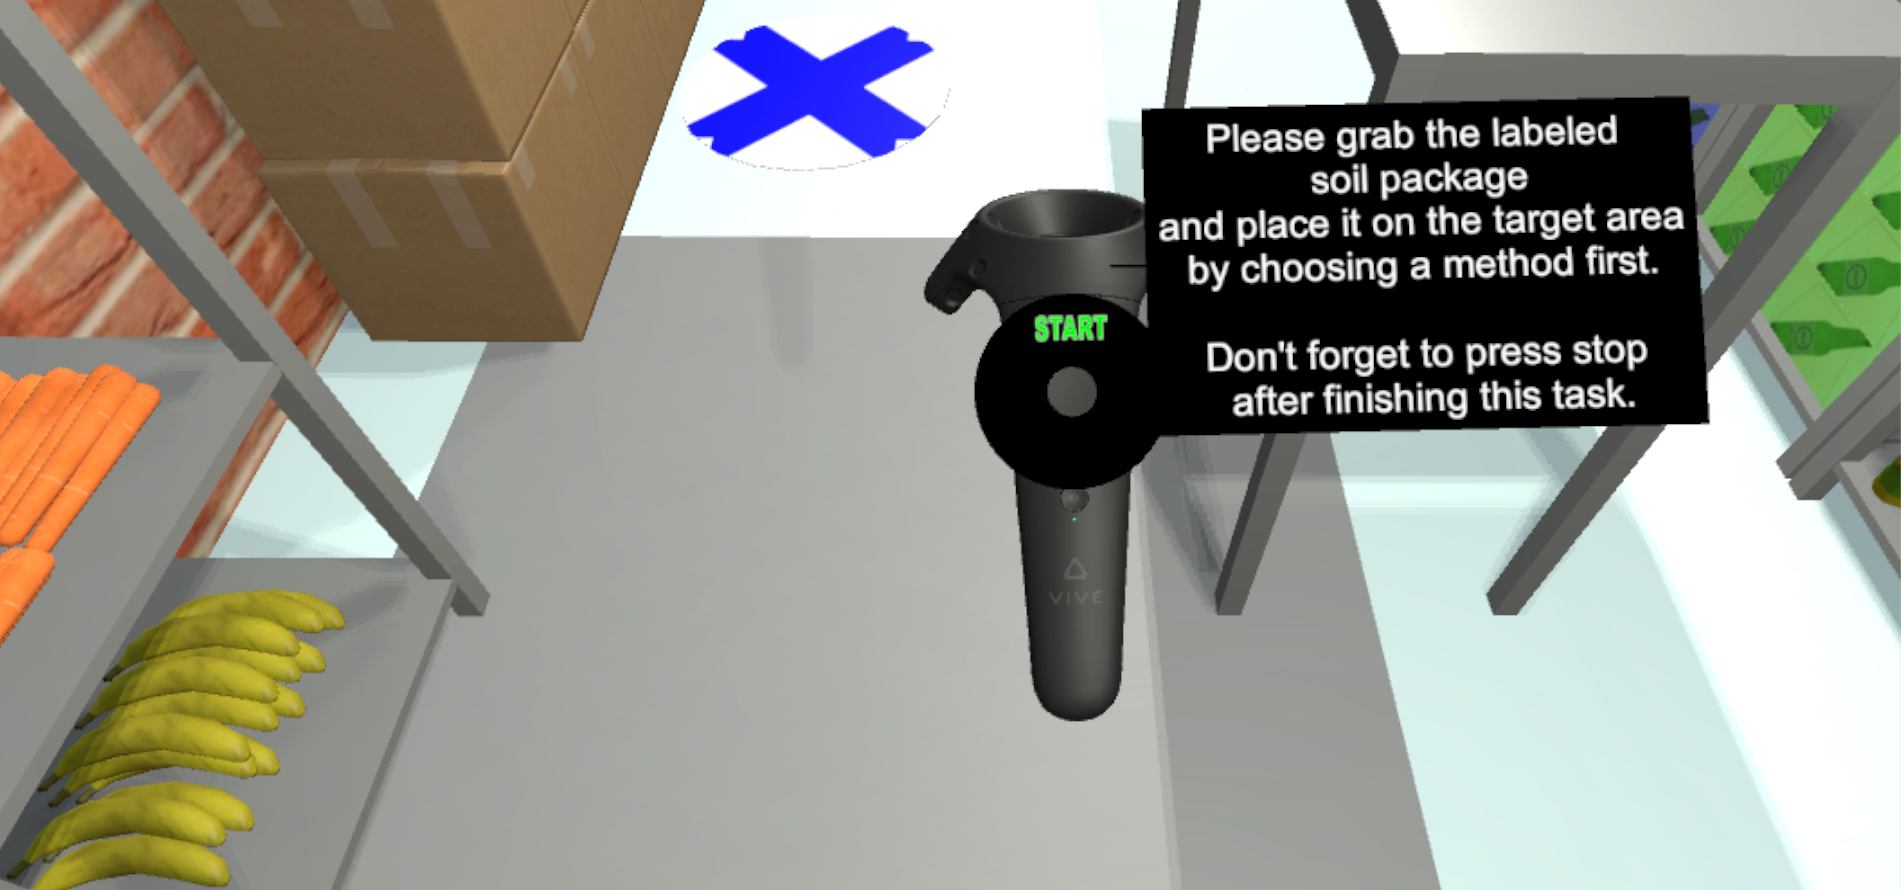
\includegraphics[width=12cm]{Images/TaskContreoller.PNG}
	\caption[Task shown next to the Controller.]{Task shown net to the Controller.}
	\label{fig:taskC}
\end{figure} 

The text for the tasks are saved in a CSV-file, similar to the selfteaching, see section \ref{sec:selfteaching}. The implementation is also comparable to the selfteaching and implemented in the script \textit{showTasks.cs}.

\begin{figure}[H] 
	\center 
	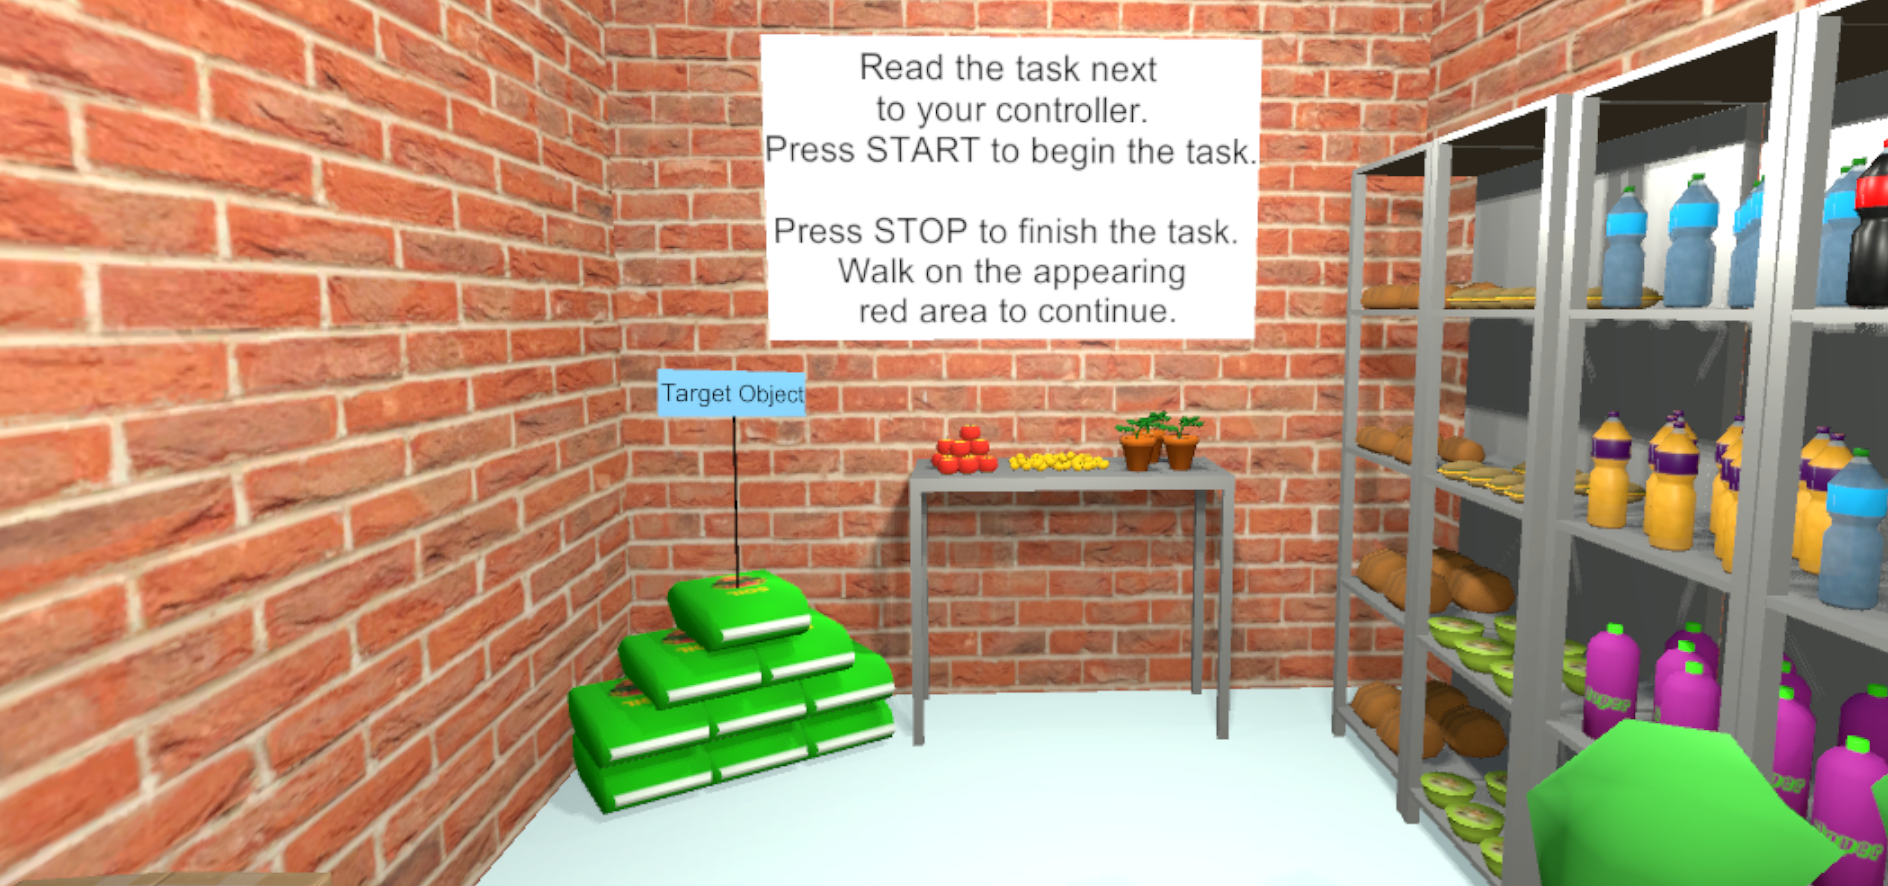
\includegraphics[width=12cm]{Images/TaskWall_1.PNG}
	\caption[Additional Information on the Wall.]{Additional Information on the Wall.}
	\label{fig:taskW1}
\end{figure}

To give the user some more instructions a information board within the supermarket is established, see figure \ref{fig:taskW1}. For the first three tasks there are only shown some basic information.\\
The last tasks will be repeated with every available method. That means, that the user has to pick up the same object five times. This object is placed, so that the user could use CR as well as FR methods (compare section~\ref{sec:Interactions}. The methods are implemented in a fif order, which can be seen in table \ref{tab: OrderMethods}. The methods will already be activated as soon as the user presses start. \\

\begin{table}[h]
\centering
 \begin{tabular}{|c|c|}
  Number of subtask & Method  \\ \hline
  1 & Close Range: Touch Grab  \\
  2 & Close Range: Wand Grab  \\
  3 & Far Range: Extendable Ray  \\
  4 & Close Range: Proximity Grab  \\
  5 & Far Range: Raycast \\
   \end{tabular}
  \caption[Order of methods in the Last Tasks.]{Order of methods in the Last Tasks.}
	\label{tab: OrderMethods}
 \end{table}

To help the user to figure out what method is activated the name of the method will be shown on the information board as soon as  he/she is in the new scene (compare figure~\ref{fig:taskW2}). 

\begin{figure}[H] 
	\center 
	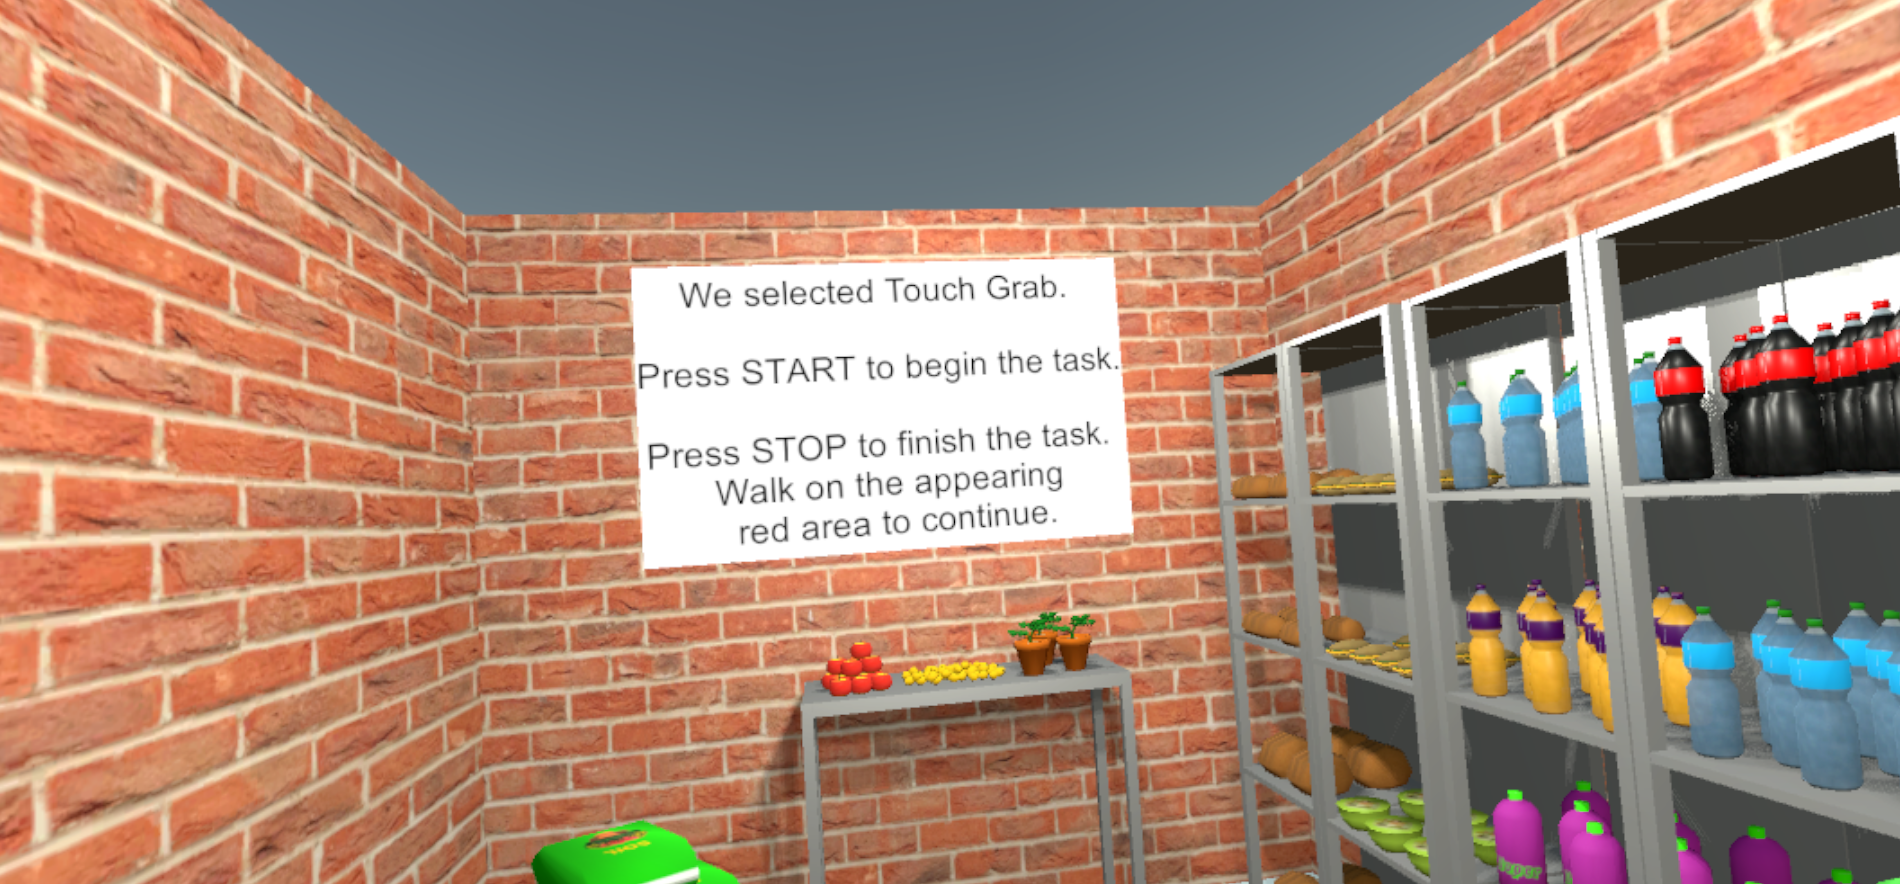
\includegraphics[width=12cm]{Images/TaskWall_2.PNG}
	\caption[\textit{Touch Grab} is activated.]{\textit{Touch Grab} is activated.}
	\label{fig:taskW2}
\end{figure}

For the last tasks a usability questionnaire needs to be answered by the user, after he/she finishes the task. 


\subsection{Measurement} \label{sec:measurement}

\subsubsection{Time and Precision Measurement}
\todo[inline, color=yellow]{Vera}
As mentioned in section \ref{sec:tasks}, several tasks must be done by the users which are designed to evaluate various aspects. Thus, three different sets of measurements could be saved automatically in a task. All results are stored in a comma separated value text file that is named after their subtask and stored directly into the unity project folder. These files could be imported in all common statistic applications like \textit{MS Office Excel}, for example. Hence, the provided template is a \textit{Excel} file with the required basic statistic computations and visualisation of the results. Here, the output files could be easily integrated in the designated table fields. Following this, the template computes all useful mean values and standard deviations of the measurements. In other cases, it calculates the percentagewise proportion like the commonness of a method use. Each calculation is displayed in a corresponding diagram. Further, the ones that visualise the mean values includes an error bar that depends on the standard deviation. If necessary, other static computation like a significance test needs to be extended because the calculation highly depends on the study conditions and are not predictable.

The first measuring set is made for the learning procedure and should evaluate the affordable learning time of a grabbing method. Therefore, their usage time is recorded during the complete learning process and saved in milliseconds when a user presses the stop button. 

Afterwards, the first task with its three subtasks is run. Here, the user's method preference of a close or far range task should be evaluated. Hence, the application measures the usage time of every selected method and saves the id of the current method when the target object is placed successfully on the target area. The listing of this measurement shows significantly which methods were preferred and if a user had comprehend their scope.  

Finally, the precision as well as the grabbing and positioning time is measured in the second task for every provided method. Therefore, the grabbing time is started when a user presses the start button and stopped when the target object is grabbed. At this point, the positioning time is started immediately and stopped when the object is placed on the target area. These time measuring should show the workload and where the users have problems with the method. Additional, the selecting and positioning error rate is recorded during the whole process. Thus, this recorded data gives conclusions about the precision. The success of this task is recorded and the use of the snapping mode, too. Hence, all relevant informations are provided to get all important conclusions about the applicability of each method. 

\subsection{Questionnaires} \label{sec:questionnaires}

\textcolor{red}{Hier wäre es generell schöner einen flüssigere Überleitungen zuschreiben. Meisten benutzt du drei bis viermal hintereinander "The" als Textanfang oder immer gleiche Satzmuster wie z.b. THe evaluation Formula... is intergrated oder "This is done ... !. }
To not only use measured values to evaluate the interaction methods but also use the participants input, the participants have to fill out two kinds of questionnaires. The first one is the \textit{SUS: a 'quick and dirty' usability scale} usability questionnaire \citep{6sus}. This questionnaire consists of ten questions. It is given to the user after each task, so each user fills out the questionnaires five times, once for each interaction method. \textcolor{red}{Hier könnte man zum besseren Verständnis etwas genauer sein. Vorallem, dass der Fragebogen im zweiten Task direkt nach der Benutzung der jeweiligen Methode ausgefüllt wird.}This is done to determine the usability of each method. The investigator has to fill in two extra questions which are a testID (one number assigned to every participant) and which method was used \textcolor{red}{Wann genau muss er das machen? oder andere Reihenfolge in der Beschreibung der Fragebögen}.This is done to be able to draw an conclusion based on the used method \textcolor{red}{Vorschlag: Hence, it is possible to draw a conclusion based on the used method.}  \\ 

The second questionnaire is a simulator sickness questionnaire by Kennedy et al. \citep{ssq} which evaluates the general discomfort caused by the virtual reality application. The investigator has to fill in the testID corresponding to the testID used for the usability questionnaire \textcolor{red}{Hier könnte man auch schreiben: This questionnaire has to be handed to the participant after all tasks are completed and the corresponding testID is entered by the investigator. Oder so ähnlich. Auf jeden Fall nicht dreimal "The" am Satzanfang}. \\

The \textcolor{red}{Durch All ersetzen?} questionnaires can either be used in a printed paper form or the provided \textit{Google Forms} can be utilized on a mobile device. When done in \textit{Google Forms}, the result can be imported into \textit{MS Office Excel}. Moreover, evaluation templates are provided as \textit{Excel} files with basic statistic calculations and visualisations. The evaluation formula \textcolor{red}{Besser: calculations or computations} of the simulator sickness questionnaire are integrated and could be easily applied to larger study groups. The result consists of four values: nausea, optic, disorientation and the total score. The total score has a range from 0 to 160.7, but a theoretical result of over 100 would be so dangerous that an ambulance should be called. \\
The evaluation formula for the usability questionnaire is also integrated. The resulting value has a range from $0$ to $100$ whereas a value of $100$ is considered for a perfect system. Above 70 are systems with good usability and a score under 50 indicates huge deficit in usability. \textcolor{red}{Vorschlag: In general, systems with a value of more than 70 seems to have a good usability and systems wit a score under 50 have a huge deficit.}\textcolor{red}{Wieder Viermal "The am Anfang :-("}




\newpage
\section{Project Management} \label{sec:pm}
\todo[inline, color=yellow]{Vera}

This chapter describes the project planning and management of the \textit{Interaction Lab}. It is divided into the different project phases. Each division includes all important facts of its project period.

\subsection{Project Definition} \label{sec:PMProjectdefinition}
\todo[inline, color=yellow]{Vera}
This section describes the results of the project definition phase in detail. This includes a problem analysis, a list of objectives and requirements, a solution concept as well as a workability analysis.

\subsubsection{Problem Analysis}\label{sec:PMProblemAnalysis}
\todo[inline, color=yellow]{Vera}
The demand for Virtual Reality (VR) devices and applications increased heavily since the first consumer devices like \textit{HTC Vive} and \textit{Oculus Rift} were released during last years. One main difficulty of the current development of VR-applications is the lack of standardisation of the Software Development Kit (SDK) and interfaces. The most acknowledged suppliers \textit{HTC} and \textit{Oculus} do not work together or force standards for VR application development. Thus, all applications are system related and incompatible with other devices. Accordingly, each device offers different opportunities of interaction methods. These methods could be divided in the acknowledged categories selecting, grabbing, manipulating, movement and indirect controlling via widgets, gestures and voice input. Several suppliers currently offer different devices for interaction. And with focus on the grabbing and positioning methods, the most common are the \textit{Oculus}-HMD, \textit{HTC Vive}-HMD, \textit{HTC Vive}-Controller, data gloves and motion capturing systems for hand-tracking like the \textit{LeapMotion}-Controller.

As mentioned in section \ref{sec:Motivation}, there exist currently no interaction laboratory which compares the different interaction methods in a scientific and credible way. Hence, the development of a virtual laboratory is highly requested to compare and test different interaction methods in adequate test environments. Thus, user friendly interaction methods which nearly full-fill usability requirements could be improved by researcher which yields to a higher demand of VR devices and application. That will squeeze the profit of VR device suppliers which include those user friendly interaction methods. 

\subsubsection{Usage Context}\label{sec:PMUsageContext} 
\todo[inline, color=yellow]{Vera}
Hence, the required laboratory has mainly two usage contexts. First, it could be used to run scientific studies in VR research or development. Second, it could demonstrate and exemplify the differences of grabbing interactions in education proposes or support the students to develop and test grabbing methods on their own during lectures. 

\subsubsection{Objective and Requirements}\label{sec:PMRequirements}
\todo[inline, color=yellow]{Vera}

At least two scenes should be realised to provide a laboratory which allows to run scientific and reliable study as well as is useful for the education of students. In the first scene, the user will be able to learn the offered grabbing methods. Therefore, this room is will provide simple cubes of various sizes which are in different distances from the users. Every cube is moveable and could be placed at every place. Each user is forced to follow the introductions of a self teaching before every offered method could be tested independently. The current user can only begin with the actual study after every method is trained to ensure equal preconditions.

The second room will be modelled after a supermarket because this model offers various options of grabbing and positioning tasks. In this room, the participant will get different tasks which will differ by complexity, distance of grabbing and size of the objects. The user will be able to change the options of grabbing independently but not choose the current method. An optional extension of the project will be another type of task where the user decides which type of method is preferred for this task.

The grabbing methods can be categorised into close range and far range and include the grabbing, rotating, and positioning of an object. Possible types of close range methods, are the actual touching of a movable object to select it or by holding the controller in the proximity of it but without touching it. Another more precise option is the selection with a thin wand in front of the controller. This of collection of methods that includes close human cognition methods as well as less or very accurate ones. 
The far range interaction will have different options as well. One will be a ray that shoot out of the controller, another one will extend a ray from the head and the third one will extend the arm in the pointed direction. This means the user will be able to point at an object with the controller or to look in the direction of it.

The system offers two measurements and the related saving of the different parameters. First, the duration time is measured for every performed task to compare and validate the performance of the different interaction methods. Second, every single grabbing try of a task will be counted and saved to get a conclusion about the learn-ability, accuracy, and performance.

Furthermore, there will be a questionnaire designed to give the users of \textit{Interaction Lab} an usability evaluation tool at hand. This questionnaire will test parameters as tiring, learnability, self-descriptiveness and fulfilling expectations.


\subsubsection{Solution Concept}\label{sec:Projectconcept}
\todo[inline, color=yellow]{Vera}
An interaction laboratory for grabbing and positioning interactions at close or far range will be developed in \textit{Unity}. It includes two test rooms e.g. scenes, where the first is a learning room, in which the users can get familiar with the interaction methods. The second room is designed as a supermarket. This environment was chosen because it offers various possibilities of exercises under changing difficulties like grabbing small mushrooms, fetching distantly placed tins or putting goods on provided target areas. The exercises are offered in form of a tasks that tells the participant what goods have to be grabbed and repositioned. These various tasks are predefined and cover all difficulties that a type of grabbing method could have. They are displayed on tables which are connected to the controller and could be shown or hide in the controller menu. 

All rooms are implemented in Unity and the VR components are controlled by the same framework. Further, the \textit{HTC Vive}-HMD and the corresponding controllers are used to run the interactions, imaging and orientation in the environment. It is planned to realise at least six interaction methods of grabbing and positioning. Additional, the complete framework should be compatible with new test scenes and other interaction categories. 

The system offers a measurement of the accuracy as well. A time measuring of duration and an error rate for every performed task is planned. Each measuring of every room is automatically saved in an output file which could be easily imported in common statistic tools. Furthermore, there will be a validated questionnaire designed to give the users a usability and simulator sickness evaluation tool at hand. This usability questionnaire will test parameters as tiring, learn-ability, self-descriptiveness and fulfilling expectations of each method. Whereas the simulator sickness evaluation asks for motion sickness and other system properties of the complete system. All questionnaires are validated and fit the requirement of VR systems and application. The results of each questionnaire will be saved in an output file as well.

\subsubsection{Workability Analysis}\label{sec:PMworkabilityAnalysis}
\todo[inline, color=yellow]{Vera}
There are several risks according to the concept in section \ref{sec:Projectconcept}. First, the measurements could be implemented incompletely or inaccurately. This can be avoided by a thorough testing before the final release with some external test persons. The tasks could be incomprehensible for them as well which should be prove as well.
The system integration future extensions could cause trouble. Therefore, the systems architecture should be designed wisely and consequently to avoid incompatibilities. Another risk of the implementation is that they might be more costly and complex as recommended but this is widely acknowledged. After the implementation is finished the interaction method performance or validation could be too expensive which results in a higher latency. These circumstances must be observed during the implementation and testing. Due to the high workload of the testing, the time slot for it and the trouble shooting might be underestimated. Another time risk is that there is limited access to the facilities and VR laboratory because of the huge number of running project at the current time.

Nevertheless, the concept is feasible and the project goals could be achieved during the time schedule because all the risk seems to manageable and could be observed during the scheduled testing.

The demand of the students project are satisfied and a financial profitability check is not necessaries due to the fact that the facilities of the university can be used and no further purchases are affordable.


\subsubsection{Project Organisation}\label{sec:PMProjectOrganisation}
\todo[inline, color=yellow]{Vera}

The project manager is Vera Brockmeyer who mainly should manage the appointments and facilities as well as to communicate to the outside. The latter is done via email or in a meeting with the concerned persons. Another task is to create and maintain the project plans that includes to keep the overview of the complete project progress and to ensure the milestones.
The current state should be hand out weekly to the team in form of an email or a team meeting.

All other team members have their own responsibilities. Anna is head of the scene building which includes the definition of the general scene design, research, and to inform the project manager about current problems and timing. The latter two points concern each head of a section. The other section is split into the close and far range interactions. The head of close range interaction is Britta Boerner and the other is Laura Anger. Both manage the implementation of their section.

The formal an informal non-verbal communication in the team is done via email with the subject \textit{VR Interface Lab} and a \textit{Google Calendar} is exclusively maintained by the project manager where all team appointments are intercalated. This calendar shows the availability of all team members and the VR laboratory, too. More complex problems or team decisions are made in the weekly team meeting with stringently required appearance. Due to the requirements and availability of the team members, the meeting is held via \textit{Skype} or in personal.

All files belonging to the project are organized in a cloud folder of \textit{Google Drive} or in two \textit{GitHub} repositories. The first one is for all \textit{LaTex} files and the second manage the complete framework. Whereas the cloud folder contains presentation files, graphics and images, To-Do-List, papers and more.

The required facility is one of the VR laboratory of the faculty which should have a minimum size of $15$qm and be located in the university building. These laboratories have a complete \textit{HTC Vive}
system and a compatible computer (see Table \ref{tab:Computer}).

\subsection{Project Planning} \label{sec:PMProjectPlanning}
\todo[inline, color=yellow]{Vera}
This section list all required projects plans like a work breakdown structure, the work packages, a capacity and cost plan as well as a quality plan.
\subsubsection{Work Breakdown Structure}\label{sec:PMWBS}
\todo[inline, color=yellow]{Vera}
The work breakdown structure (see Figure \ref{fig:wbs}) is split in four groups. First, the project planning which contains the actual project management as well as the research work packages Second, the implementation group includes the development of the laboratory environment and the six interaction methods. Third, the evaluation contains the work packages of tasks including measurements and the questionnaires. Finally, the last group includes the documentation and project profile packages.

\begin{figure}[H] 
	\center 
	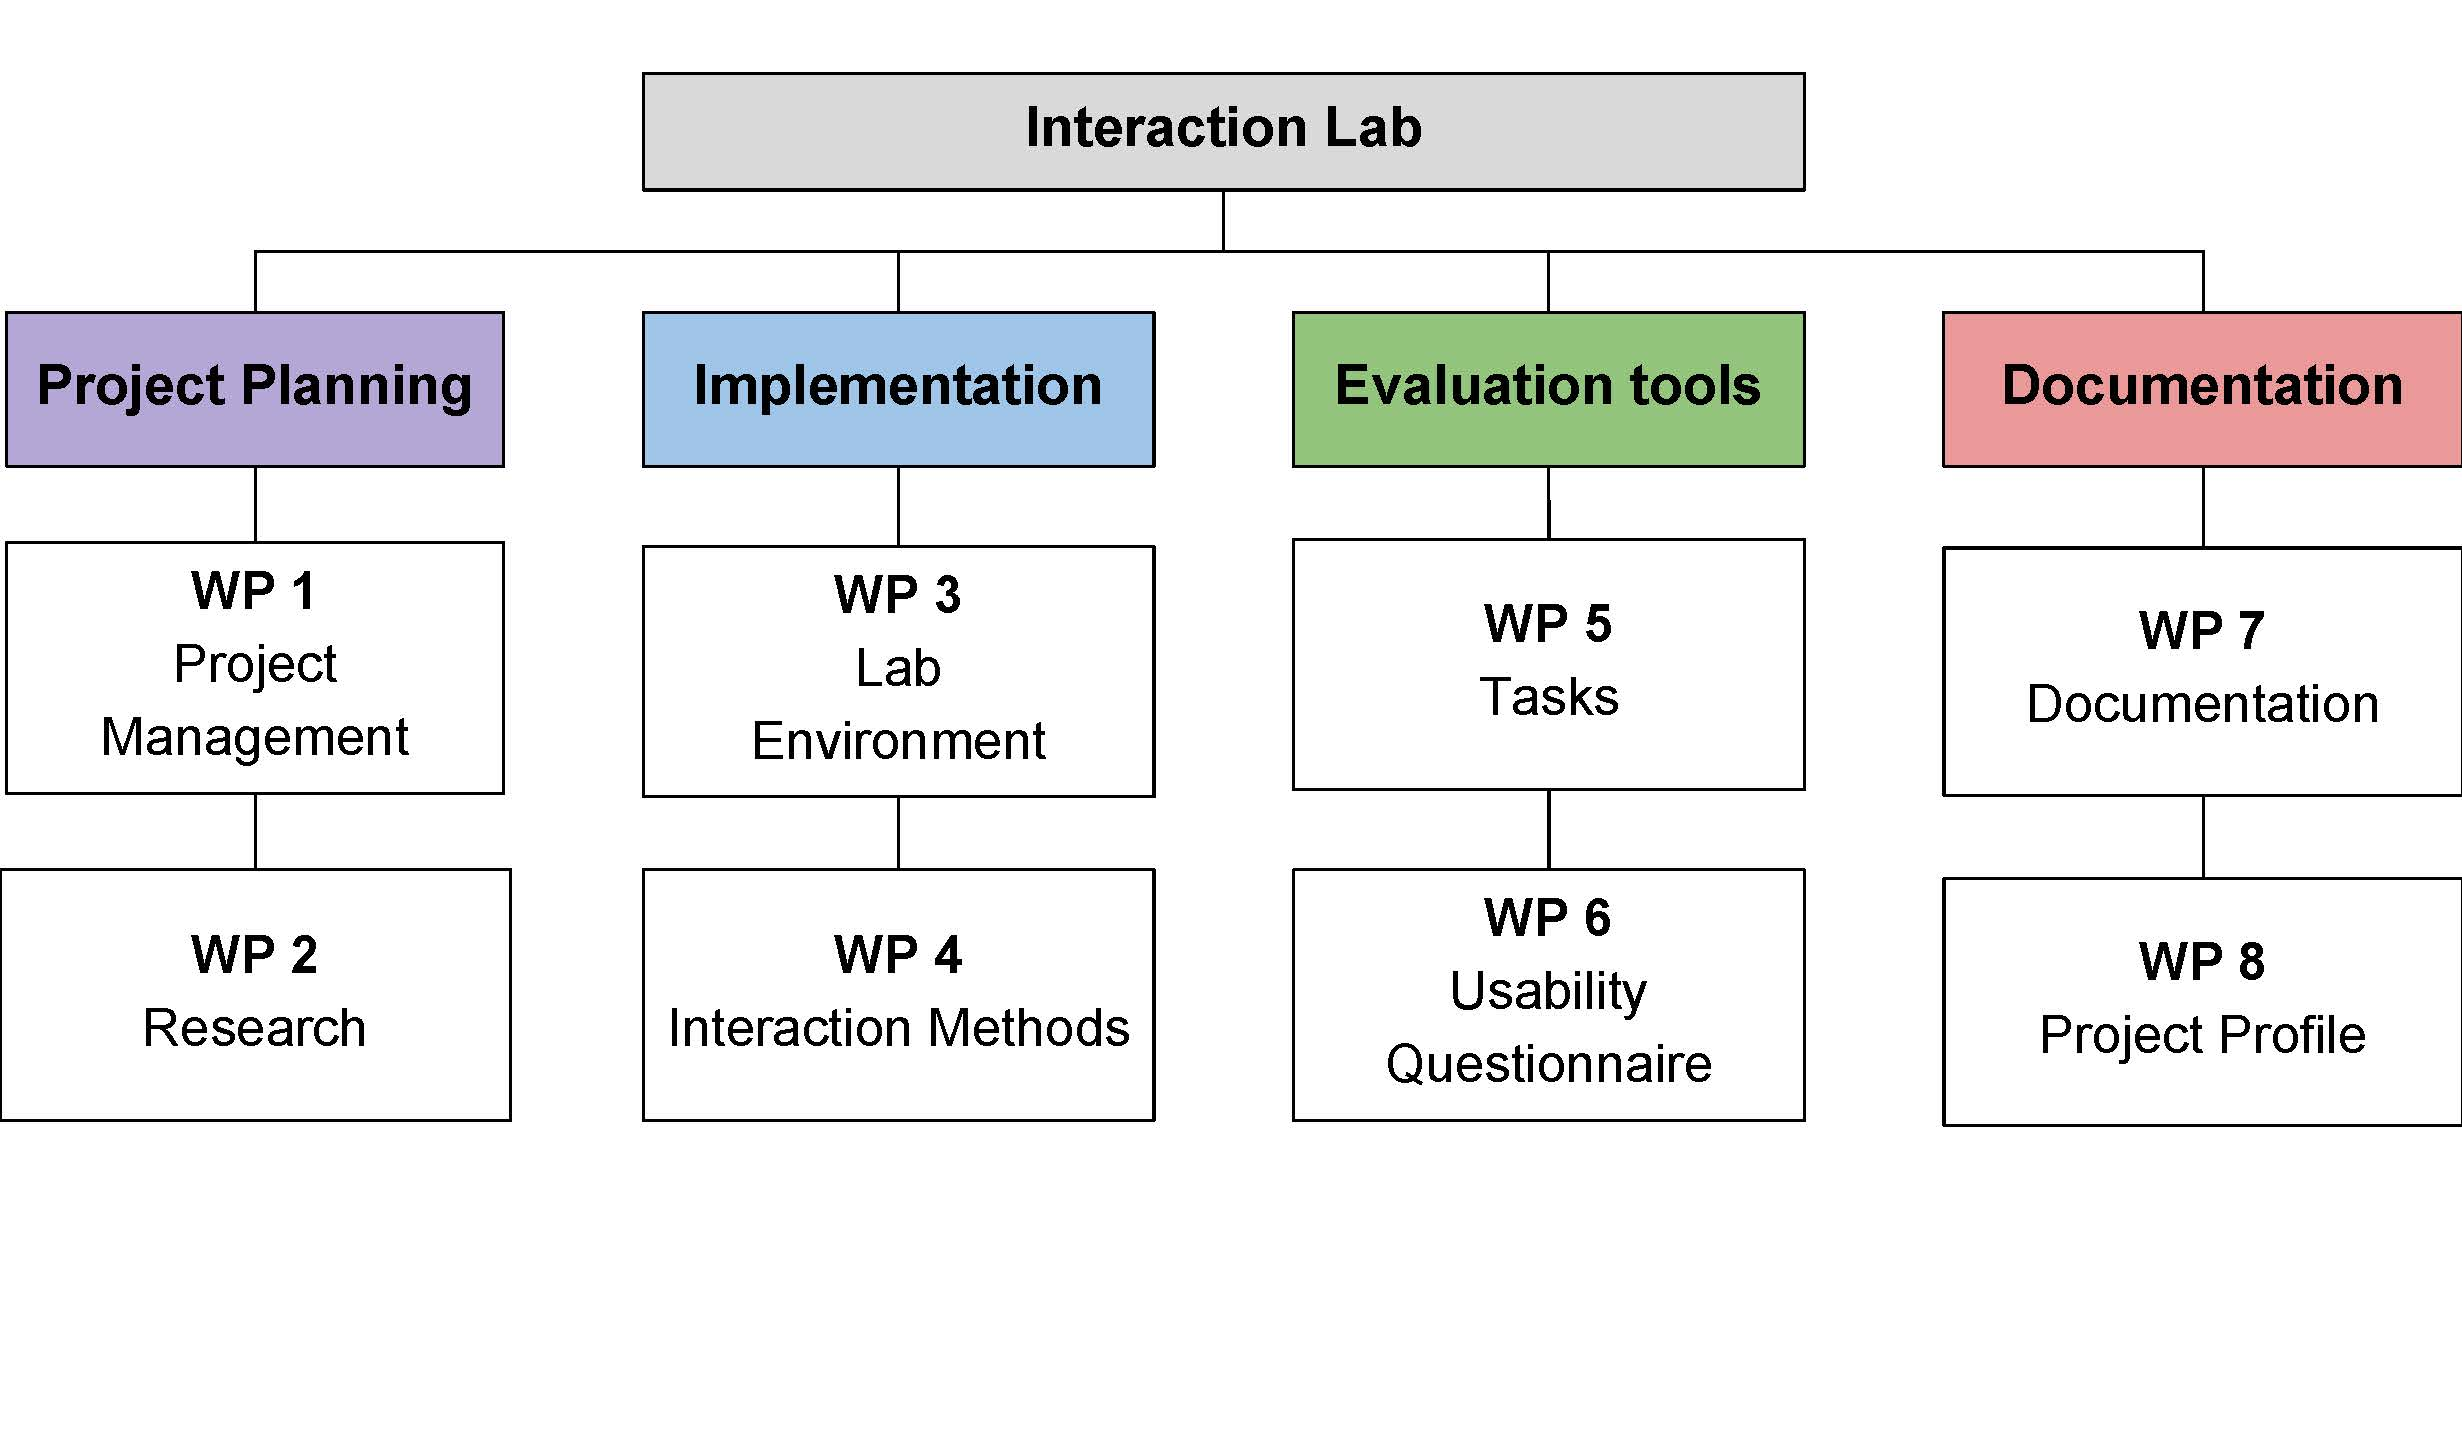
\includegraphics[width= 15 cm]{Images/WBS.jpg}			
	\caption[]{Work Breakdown Structure}
	\label{fig:wbs}
\end{figure}
\subsubsection{Workpackages}\label{sec:PMWorkpackages}
\todo[inline, color=yellow]{Vera}
A complete listing of the work packages according to Figure \ref{fig:wbs} could be seen in the Appendix A \ref{sec:AppendixA}.

\subsubsection{Project Schedule}\label{sec:PMSchedule}
\todo[inline, color=yellow]{Vera}

Figure \ref{fig:wbs} shows the project schedule with the timing of all work packages. The most important deadlines are the project plan, research, first and second prototype as well as the release deadline. First, the project plan should be finished until 13th April 2017. Second, the research deadline is two and a half weeks later at the 27th April 2017. Followed by both prototypes which are set for the 31st may and 30th June 2017. The final release deadline is at the 15th July 2017.

\begin{figure}[H] 
	\center 
	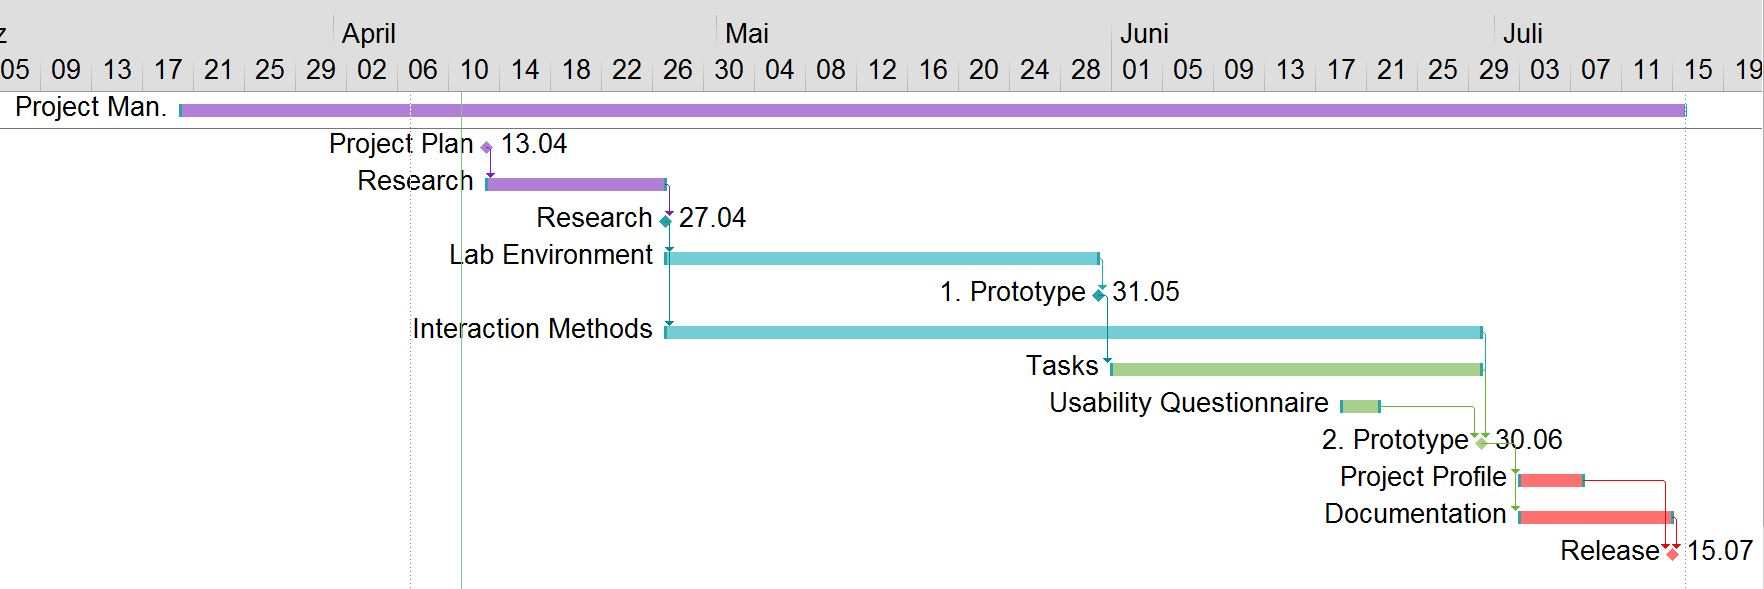
\includegraphics[width= 15 cm]{Images/Gantdiagramm.jpg}			
	\caption[]{Project Schedule}
	\label{fig:wbs}
\end{figure}

\subsubsection{Capacity Plan}\label{sec:PMCapacity Plan}
\todo[inline, color=yellow]{Vera}

The capacity plan lists the estimated time resources of each team member, the availability of the required laboratory with the \textit{HTC Vive} system and the SLR camera for the documentation.
\begin{table}[H]
	\centering
	\begin{tabular}{|l|l|l|l|}
		\hline
		\Absatzbox{}
		\textbf{Resource} &	\textbf{ Estimated [h]} &	\textbf{Actual [h]} & 	\textbf{Buffer [$\%$]}\\ \hline
		Laura &	166 &	180	& 7.78\\ \hline
		Anna&	170	&180&	5.56\\ \hline
		Vera&	182	&180&	-1.11\\ \hline
		Britta&	168&	180	&6.67\\ \hline
		Total Personal&	686	&720&	4.72\\ \hline
		VR Lab 1&	173&	152&	-13.82\\ \hline
		SLR Video Camera&	8&	8&	0.00\\ \hline
	\end{tabular}
	\caption[]{Capacity Plan of personal and facility resources.}
	\label{tab:Capacity Plan}
\end{table}

\subsubsection{Cost Plans}\label{sec:PMCostPlan}
\todo[inline, color=yellow]{Vera}

The cost plan of personal resources in Table \ref{tab:Personal Cost Plan} gives a more detailed overview of the estimated time resources per work package. It is structured into the cost of each team member and the total cost of a work package. Whereas, the cost plan of the facility resources offers an overview of the material costs and their providers.

\begin{table}[H]
	\centering
	\begin{tabular}{|p{5cm}|p{1.5 cm}|p{1 cm}|p{1cm}|p{1.5 cm}|p{2 cm}| l l l l l l }
		\hline
		\Absatzbox{}
	\textbf{Name}&	\textbf{Laura [h]} &\textbf{Anna [h]} &	\textbf{Vera [h]} &\textbf{	Britta [h]} &	\textbf{Cost WP [h]} \\ \hline
	Project Management &	12&	12&	45&	12&	81\\ \hline
	Research&	10	&10	&10&	10	&40\\ \hline
	Lab Environment&	0&	55&	32	&10&	97\\ \hline
	Interaction Methods	&65&	0&	0&	65	&130\\ \hline
	Tasks	&15&	45	&30&	15&	105\\ \hline
	Usability Questionnaire	&8	0&	0&	0&	8\\ \hline
	Documentation	&45	&45&	55&	45&	190\\ \hline
	Project Profile	&8	0&	0&	8&	16\\ \hline
	\textbf{Total Cost}	&\textbf{163}&	\textbf{167}	&\textbf{172}&	\textbf{165}	&\textbf{667}\\ \hline
	
	\end{tabular}
	\caption[]{Cost Plan of personal resources.}
	\label{tab:Personal Cost Plan}
\end{table}

\begin{table}[H]
	\centering
	\begin{tabular}{|p{3cm}|p{1 cm}|p{1.5 cm}|p{1.5cm}|p{1.5 cm}|p{3.5 cm}| l l l l l l }
		\hline
		\Absatzbox{}
		\textbf{Ressourcen}	&\textbf{Quan- tity}&	\textbf{Unit Price [EUR]}&	\textbf{Cost [EUR]}&\textbf{Act. Cost [EUR]}&\textbf{Comments} \\ \hline
			 HTV Vive &	1	&899&	899&	0	&Price of Vive Online Shop, provided by TH Cologne\\ \hline
			 SLR Camera&	1	&500&	500&	0	&estimated, provided by team member\\ \hline
			 VR Computer&	1	&1800&	1800	&0	&offer from Computer Shop, provided by TH Cologne\\ \hline
			 MS Office	&1	&149&	149&	0&	provided by TH Cologne\\ \hline
			MS Project&	1	&195&	195&	0&	provided by TH Cologne\\ \hline
			3D assets of Food Beverages&	2&	15&	30&	0	&Steam\\ \hline
	\textbf{Total}	&	& &	\textbf{3573}	&\textbf{0}	&\\ \hline
		
	
	\end{tabular}
	\caption[]{Cost Plan of facility resources.}
	\label{tab:facility Cost Plan}
\end{table}


\subsubsection{Quality Plan}\label{sec:PMQualityPlan}
\todo[inline, color=yellow]{Vera}
\begin{table}[H]
	\centering
	\begin{tabular}{|p{3cm}|p{3 cm}|p{3.5 cm}|p{3.5cm}|}
		\hline
		\Absatzbox{}
		\textbf{Quality Goal}&	\textbf{Criteria} &\textbf{Method} &	\textbf{Controlling}\\ \hline
	Immersion and Presence	& no distraction by real world &	Presence questionnaire by Witmer and Singer; questions according to sound and haptic will left out	& use and evaluate brief questionnaire during functionality test\\ \hline	
Low Latency	& under $20$ms &	keep the scenes as simple as possible & show the frames per second in the Unity console\\ \hline		
No dropouts	& no black frames or errors in the unity project & no expensive or parallel calculation & visual testing\\ \hline	
Understandability of tasks	& correct task performance by test user during functionality tests & use common objects and tasks; brief and precise task descriptions & use brief questionnaire during functionality test\\ \hline	
robust system & Vive System does not crash during process & no expensive calculations; control and calibration of hardware; analyse and solve directly problems & observe during development
\\ \hline
Correct saving of Usability Questionnaire Response & entire answers of study participants are correctly saved in an file & Use of Google Forms & functionality test and controlling of completeness and correctness\\ \hline
Understandability of Usability Questionnaire & no questions or uncertainties of test users& validated Usability Questionnaire & use and evaluate brief questionnaire during functionality test\\ \hline
	\end{tabular}
	\caption[]{Quality Plan}
	\label{tab:Qaulity Plan}
\end{table}
\subsection{Project Execution} \label{sec:ProjectExecution}
\todo[inline, color=yellow]{Vera}
The following sections summarizes the project progress as well as the problems that caused a delay of the schedule.
\subsubsection{Project Progress}

In general, the project progress went off quite well and most of the project goals were achieved and are running as expected. Therefore, the \textit{Interaction Lab} is a complete and running application that includes all required tools for a scientific study. The final system contains a learning room, a supermarket test scene with implemented task and measuring, the implementation of five different interaction methods to test, completely set of validated usability questionnaires and excel templates for the evaluations.

However, some of the project goals were too ambitious for the resources capacity in the scheduled time window. Thus, not all project goals were completely achieved. First, the Gogo interaction method and the HMD raycast could not be developed due to the problems mentioned in section \ref{sec:PMProblems}. Second, the number of tasks needed to be reduced significantly because it turned out that they are too time consuming during testing. Hence, only one task was implemented with all provided interaction methods and three tasks to figure out the preferences of the users for various kind of ranges and object sizes. Third, an additional goal was set after the first prototype. A self teaching mode has been added to the learning room to ensure an equal introduction of the methods and task for each test user.

The actual workload of most work packages covers their estimation beside some problems which are described in detail in section \ref{sec:PMProblems}. All team members had a similar work load and the task allocation work efficient and well. Each team member knew their current tasks at every time and had an overview of the complete progress. This overview was achieved with weekly meetings via \textit{Skype} or if affordable in personal. Furthermore, every few weeks we had a meeting with Prof. Grünvogel to give him an update and discuss current problems and their solution.


\subsubsection{Problems and Solutions}\label{sec:PMProblems}
\todo[inline, color=yellow]{Vera}

A first problem was the additional work effort because all project plans needed to be overworked which causes a one week delay. In the end it should also be noted the planning was to detailed in the beginning which cause some unnecessary time. Thus, the research phase need to shorten and place on hold for this week but this step brought the project back on time. Another delay of one and a half week causes the inevitable unity and \textit{HTC Vive} system that were more difficult that expected. This kind of problem occurs several times when changing the laboratory due to limited capacities of the designated VR Lab 1 or the periphery of the laboratories were not present. Additional, every time the VR systems needs to be recalibrated when changing the laboratory.

The VR system causes trouble during the implementation of the HMD Raycast method, too. It turned out that the tracking of the HMD lacks of precision and the ray drifts at the border of the view field. At this point, the number of tasks that must be done to guarantee a working application until the release was challenging. Thus, we concentrate on a working application and discard the HMD Raycast. However, it seems that the implementation of the Gogo method was too complex for this time schedule, too. Hence, it was changed to the Extenable Ray method which could be implemented successfully during the calculated period. 

This decision and the resulting choice of methods had the advantage that their basic structure is adoptable. Regarding to this realisation, it could be said that the split of responsibility for Far and Close Range in the project organisation was a mistake. Accompanied with the decision to create a single C\# script per method. This plenty of scripts caused a lot of trouble during their integration in the final application but these problems were solves by using only one script for similar methods like the ray methods, for example.

\newpage


























\section{Reflection} \label{sec:Reflexion}


Finally, a running and nearly complete application was developed during this project. The test environments in form of the learning room and supermarket are working without a latency or blackouts. They provide an effective virtual laboratory that can be used by researchers or for educational purposes. Both environments integrate five perfectly working grabbing interaction methods. First, the close range methods Touch, Proximity and Wand Grab are implemented and the first two extends an optional snapping mode. Second, the two far range methods Raycast and Extendable Ray are successfully integrated into the application.
 
All measurements of the tasks are saved automatically in output files that could be evaluated with the provided \textit{MS Office Excel} template.The usability questionnaire forms could be accessed by every mobile device or computer and their results are saved automatically as well. They are offered in English and German language and could be certainly evaluated with the template, too. Additional, all required consent forms are delivered in both languages with the application as PDF file.

As mentioned in section \ref{sec:PMProblems}, the HMD Raycast and Gogo method could not be realised but unfortunately there are more goals that are not yet achieved or do not work completely without faults. First, currently the self teaching mode only works if the introductions were strictly followed. In case of a mistake it will recover only when a new method is selected. Second, there is no reminder of the usability questionnaires during the last task for the study supervisor. He is forced to be totally focused during a test. Another failure is the missing question of the VR experience in these questionnaires and the lack of the general input of the test id in the application.

There are some technical mistakes as well which are not yet fixed. A main problem is the potential loss of script links in the unity project when the laboratory is changed or a git repository is pulled. A further problem is the lack of an easy method or scene extension in the application due to the complex measuring and interaction script architecture. Other small and rare troubles are the visible ray in front of transparent surfaces or object that fall sometimes through the ground.

\newpage


























\section{Conclusion} \label{sec:Conclusion}


The project progress went well with focus on a working application and without bigger complications. These were directly discussed and solved by the team. Each team member make one's contribution in nearly equal percentages. Hence, the result is a working application for the evaluation of grabbing interaction methods with the \textit{HTC Vive} controllers. Most of the project goals were achieved beside the missing HMD Raycast and Gogo interaction method, the reduction of user tasks and the missing extensibility. Nevertheless, it has to mentioned that there is still a potential for improvement like the visible ray on transparent surfaces or the objects that sometimes fall through the ground. 

\newpage


























\section{Self-Assessment} \label{sec:SA}
\todo[inline, color=red]{???}


\subsection{Anna Bolder} \label{sec:SAAnna}
\todo[inline, color=yellow]{Anna}

\textbf{Working Ours:} \textcolor{red}{116} \\ \\
\textbf{Written Sections:} \ref{sec:SOTALabor},  \ref{sec:VRLabor} (subsections included), \ref{sec:Menu}, \ref{sec:selfteaching} and \ref{sec:tasks} \\ \\
\textbf{Responsibilities:}\\ \\
My main tasks in this project was the menu as well as the displaying of different informations, selfteaching and tasks, for the user. \\
At the beginning I created a shared Unity project and added the Steam VR plug-in. I created different rooms for the testing of the close and far range interactions. Also I designed the learning room, described in \ref{sec:Learningroom}. With V. Brockmeyer I discussed the structure of the supermarket. Additional I researched the options to switch between the rooms and created the basis for the script \textit{TargetTest.cs}.\\
After the creation of the basic scenes I researched for a solution of an radial menu on the controller. I implemented this with the ``VRTK'' plug-in. To collect all functions behind the buttons in one script I created the script \textit{menu.cs}.
As soon as all interactions were implemented L. Anger and I integrated the interactions in the menu and all scenes. Here I helped to simplify the switching between different interactions with a ray. \\
In the last weeks I implemented the selfteaching together with V. Brockmeyer. This was time-consuming because the counter has to be increased or set on different parts of the project and the height of the canvas has to be set for every step.\\
With the knowledge of the selfteaching I and L. Anger implemented also the tasks in the supermarket. Here we had to add a board on the wall and to short the actual tasks texts. \\
Also I did the test surveys together with L. Anger.\\

\textbf{Self-Reflexion:}\\ \\
In my opinion the project ran quiet well. Everybody had their part of the project and we also helped each other.\\
I underestimated some parts of my responsibilities. First the selfteaching took much more time than I expected. There were a lot more steps to do than I thought. Second the combination of all interactions in one menu and scene was more complicated. We did not think about that they could affect each other or that parts of the interaction have to be loaded at the start of the scene to work correctly.\\

\newpage
\subsection{Vera Brockmeyer} \label{sec:SAVera}
\todo[inline, color=yellow]{Vera}


\textbf{Working Ours:} 170 \\ \\
\textbf{Written Sections: }\ref{sec:Introduction}(subsections included),  \ref{sec:measurement}, \ref{sec:pm} (subsections included), \ref{sec:Reflexion}, \ref{sec:Conclusion} \\ \\
\textbf{Responsibilities:}\\ 
My main responsibility was the planning, organisation and management of the project. This includes the making of all project plans and the definition of it as well as to monitor the project progress and to guarantee the compliance of the schedule. Another task was the management of the internal and external communication as well as representation. This includes the making of appointments for meeting and required facilities as well as the steadily summary of the current project state. However, the distribution of the work tasks was my responsibility, too.

Beside the project management, I supported Anna Bolder with the implementation of the VR environment. In detail, I build the supermarket scene with 3D assets from the Steam Store and did the research for the tasks. Furthermore, I wrote all texts of the tasks and self-teaching and supported Anna Bolder with the implementation of the ladder. However, my other main task was the implementation, integration and output of the measurement. This includes the making of an \textit{MS Office Excel} template to evaluate the measuring's.


\textbf{Self-Reflexion:}\\ \\
I assume that the project worked very well without big complications that afford a time consuming solution or plenty of unnecessary work. According to the planning, it turned out that I planned to much in detail at the beginning which costs a lot of time resources and results in a complete refactoring of all plans. Another planning failure was the lack of enough research time during the complete project. 

The communication works quite well beside some small periods in the beginning where I planned too much and long team meetings and one where should have been more team meetings in May to avoid little misunderstandings. Beside this, I assume that I distribute the work tasks efficiently with regards to the skills of the team members. The external communication worked quite well beside some intermediately state of knowledges due to meetings without me. Especially, the translation of the usability questionnaires in German and the parallel decision to run the whole application in English language because of the brief schedule. 

According to my task during the development of the VR environment, I implemented a working measuring with all required output files. Nonetheless, the architecture of it do not allow an easy extension of further interaction methods or scenes. 

Briefly, the project team worked very good together and solved each problem directly with focus on the entire application without rest on details. The results correspond to our expectations besides some little failures.
\subsection{Britta Boerner} \label{sec:SABritta}
\todo[inline, color=red]{Britta}

\newpage
\subsection{Laura Anger} \label{sec:SALaura}
\todo[inline, color=yellow]{Laura}

\textbf{Working Ours:} \textcolor{red}{125} \\ \\
\textbf{Written Sections:} \ref{sec:StateOfTheArt},  \ref{sec:SOTAInteractions}, \ref{sec:System} and \ref{sec:Interactions} (subsections included) \\ \\
\textbf{Responsibilities:}\\ \\
Besides mandatory tasks, like for example doing research on specific problems and helping with the project management, I was mainly working on the implementation of the interactions. At the beginning of the project we divided the interactions into CR and FR (compare section~\ref{sec:Interactions}). At that time I became responsible for the FR methods of the \textit{Interaction Lab}. As it turned out it was not wise to distinguish between those two categories strictly, the borders of the jurisdiction of B. Boerner (Head of CR interactions) and me became more and more blurred. That is why we ended up working on most of the interaction methods together. This was more expedient, because for example the \textit{Wand Grab} (compare section~\ref{sec:WandGrab}), which is a CR interaction is very similar to the FR interactions \textit{Raycast} (compare section~\ref{sec:Raycast}) and \textit{Extendable Raycast} (compare section~\ref{sec:ExtendableRay}). Because B: Boerner went into holidays rather at the end of the implementation phase, I implemented the \textit{Wand Grab} on my own. \\
Together with A. Bolder I integrated the implemented interaction methods into the actual scenes (compare section~\ref{sec:VRLabor}) of the \textit{Interaction Lab}. We also took care of the visualisation of the tasks for the user. Therefore we created a display on the wall of the supermarket as well as next to the controller. On both of the displays the corresponding tasks are presented for the user. \\
I was also involved in creating the project video and all images for this documentation.\\
A. Bolder and I ran a test survey with 5 participants, which is described in section \textcolor{red}{???}.

\textbf{Self-Reflexion:}\\ \\
All in all I felt like the project run smoothly and well planned. Of course I was confronted with unknown terrain, as I never had implemented interactions of any kind. Maybe this was why I first started to create one script per interaction method. In the end of the project I noticed, that both Raycast methods and the \textit{Wand Grab} work after the same rules, so I combined them in one script. If I had done that earlier I could have avoided a lot of trouble for me and Anna Bolder as we needed to integrate them in to all scenes, separately first. \\
But all in all the workflow was well structured, as anyone had her own work area. Whenever this areas collides (for example the integration of the interactions into our scenes), we managed that both responsible people worked together on this task.

\newpage


























\section{Appendix}
\todo[inline, color=red]{Vera}
\subsection{Appendix A} \label{sec:AppendixA}
\begin{figure}[H] 
	\center 
	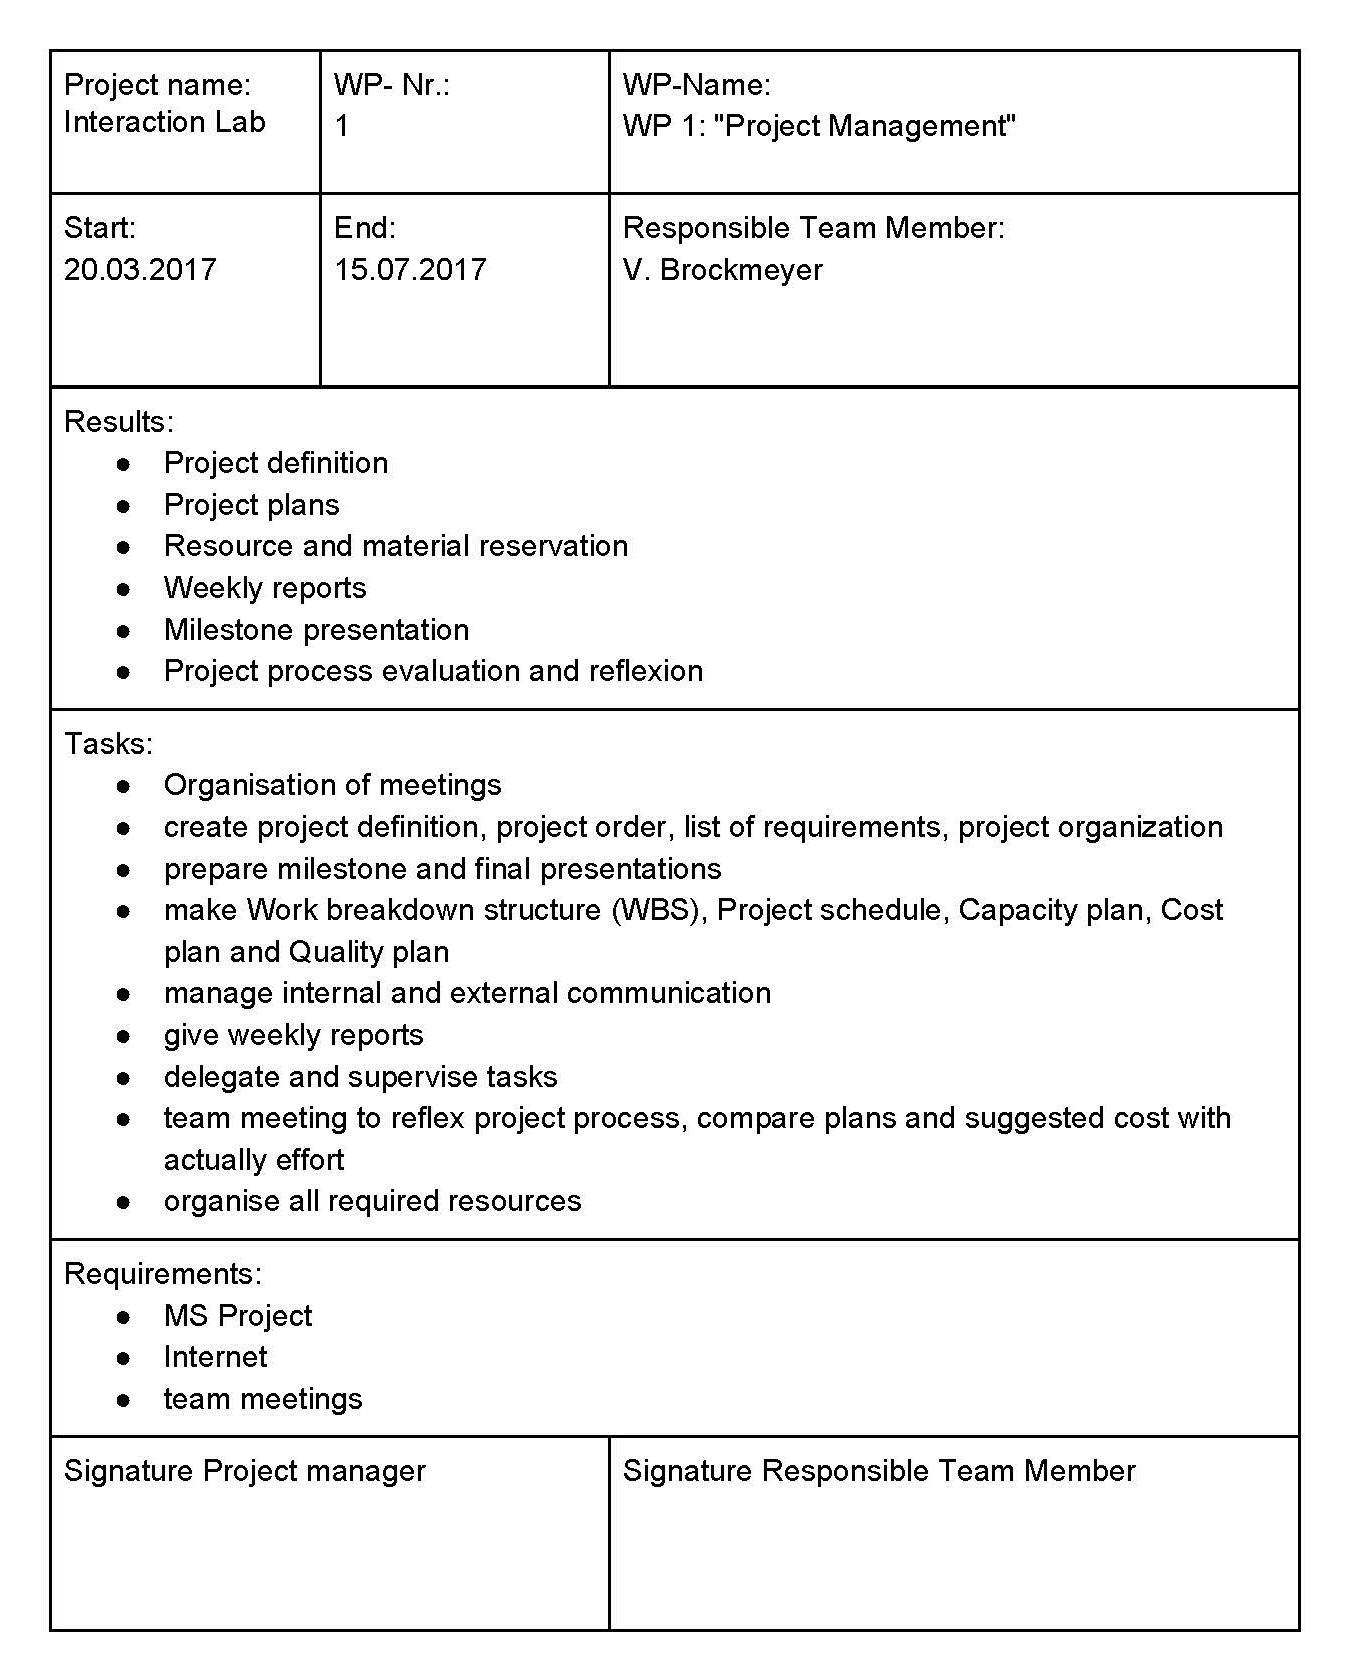
\includegraphics[width= 16 cm]{Images/Workpackages_Seite_1.jpg}			
	\caption[]{First Workpackage: Project Management}
	\label{fig:Workpackage1}
\end{figure} 
\newpage
\begin{figure}[H] 
	\center 
	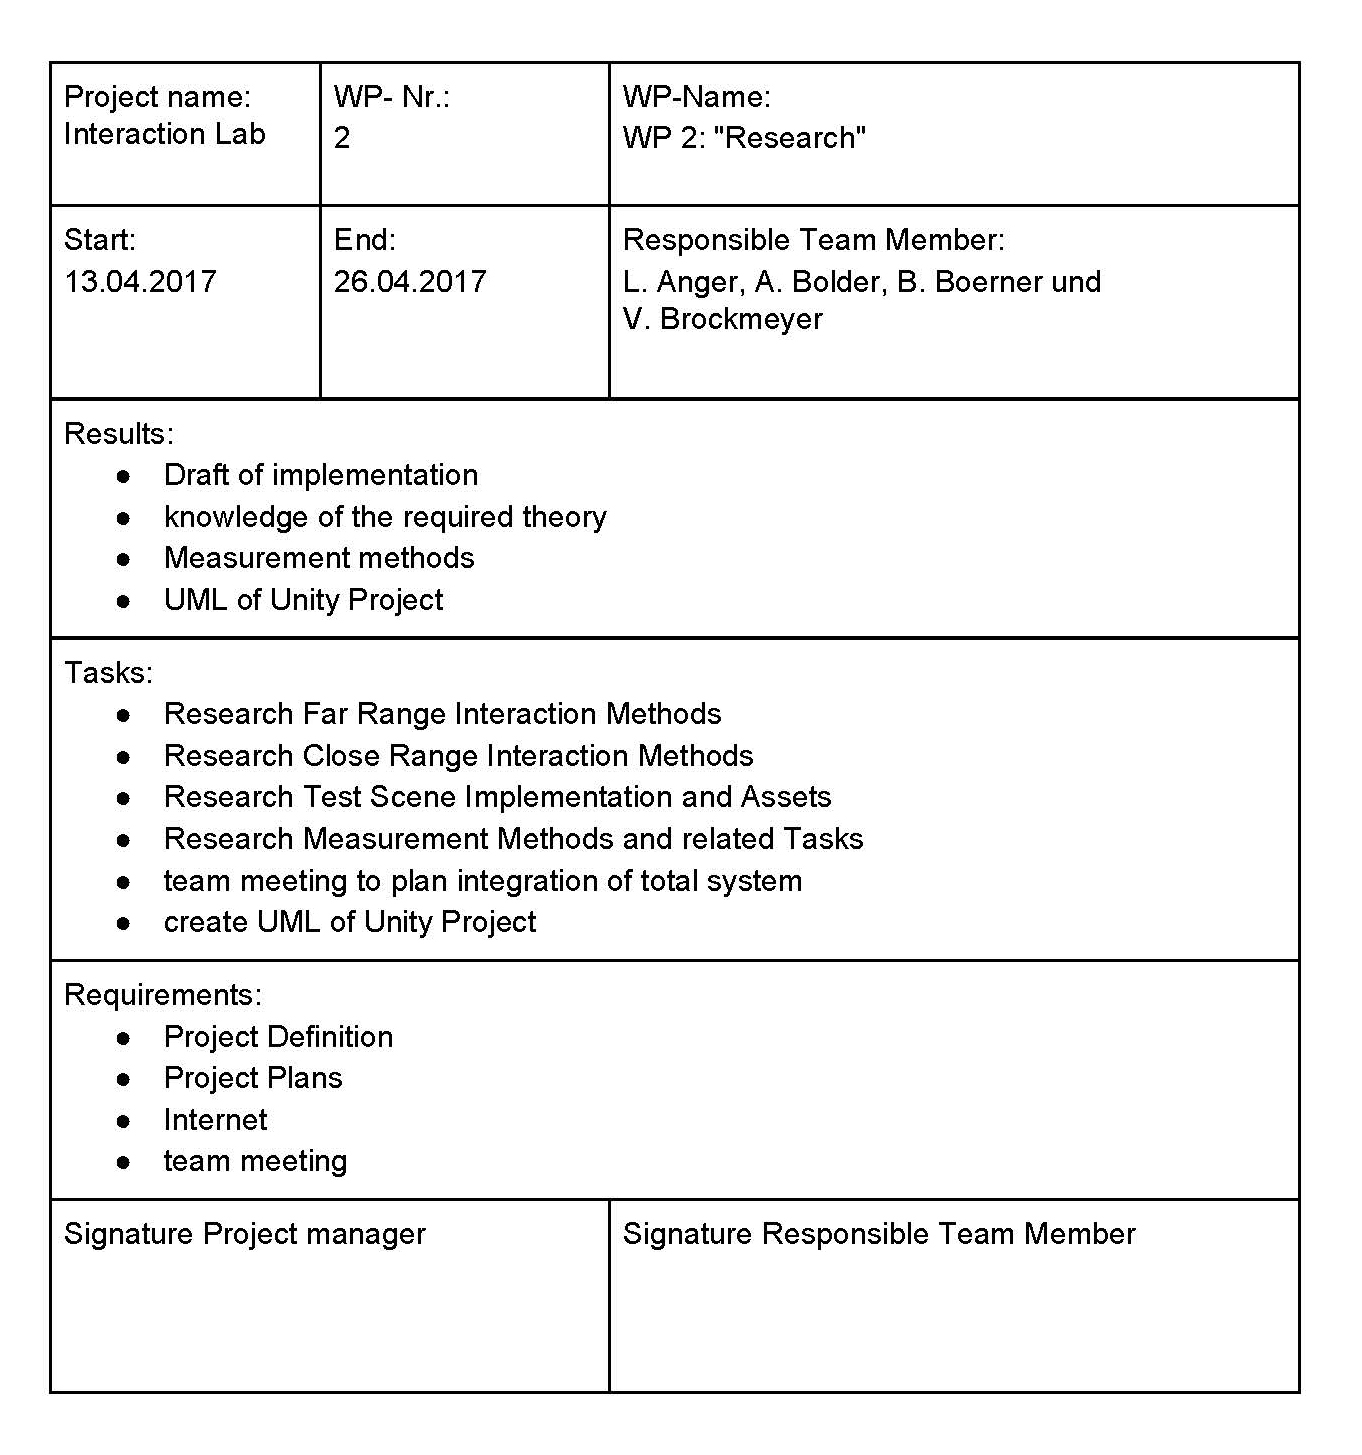
\includegraphics[width= 16 cm]{Images/Workpackages_Seite_2.jpg}			
	\caption[]{Second Workpackage: Research}
	\label{fig:Workpackage2}
\end{figure} 

\newpage
\begin{figure}[H] 
	\center 
	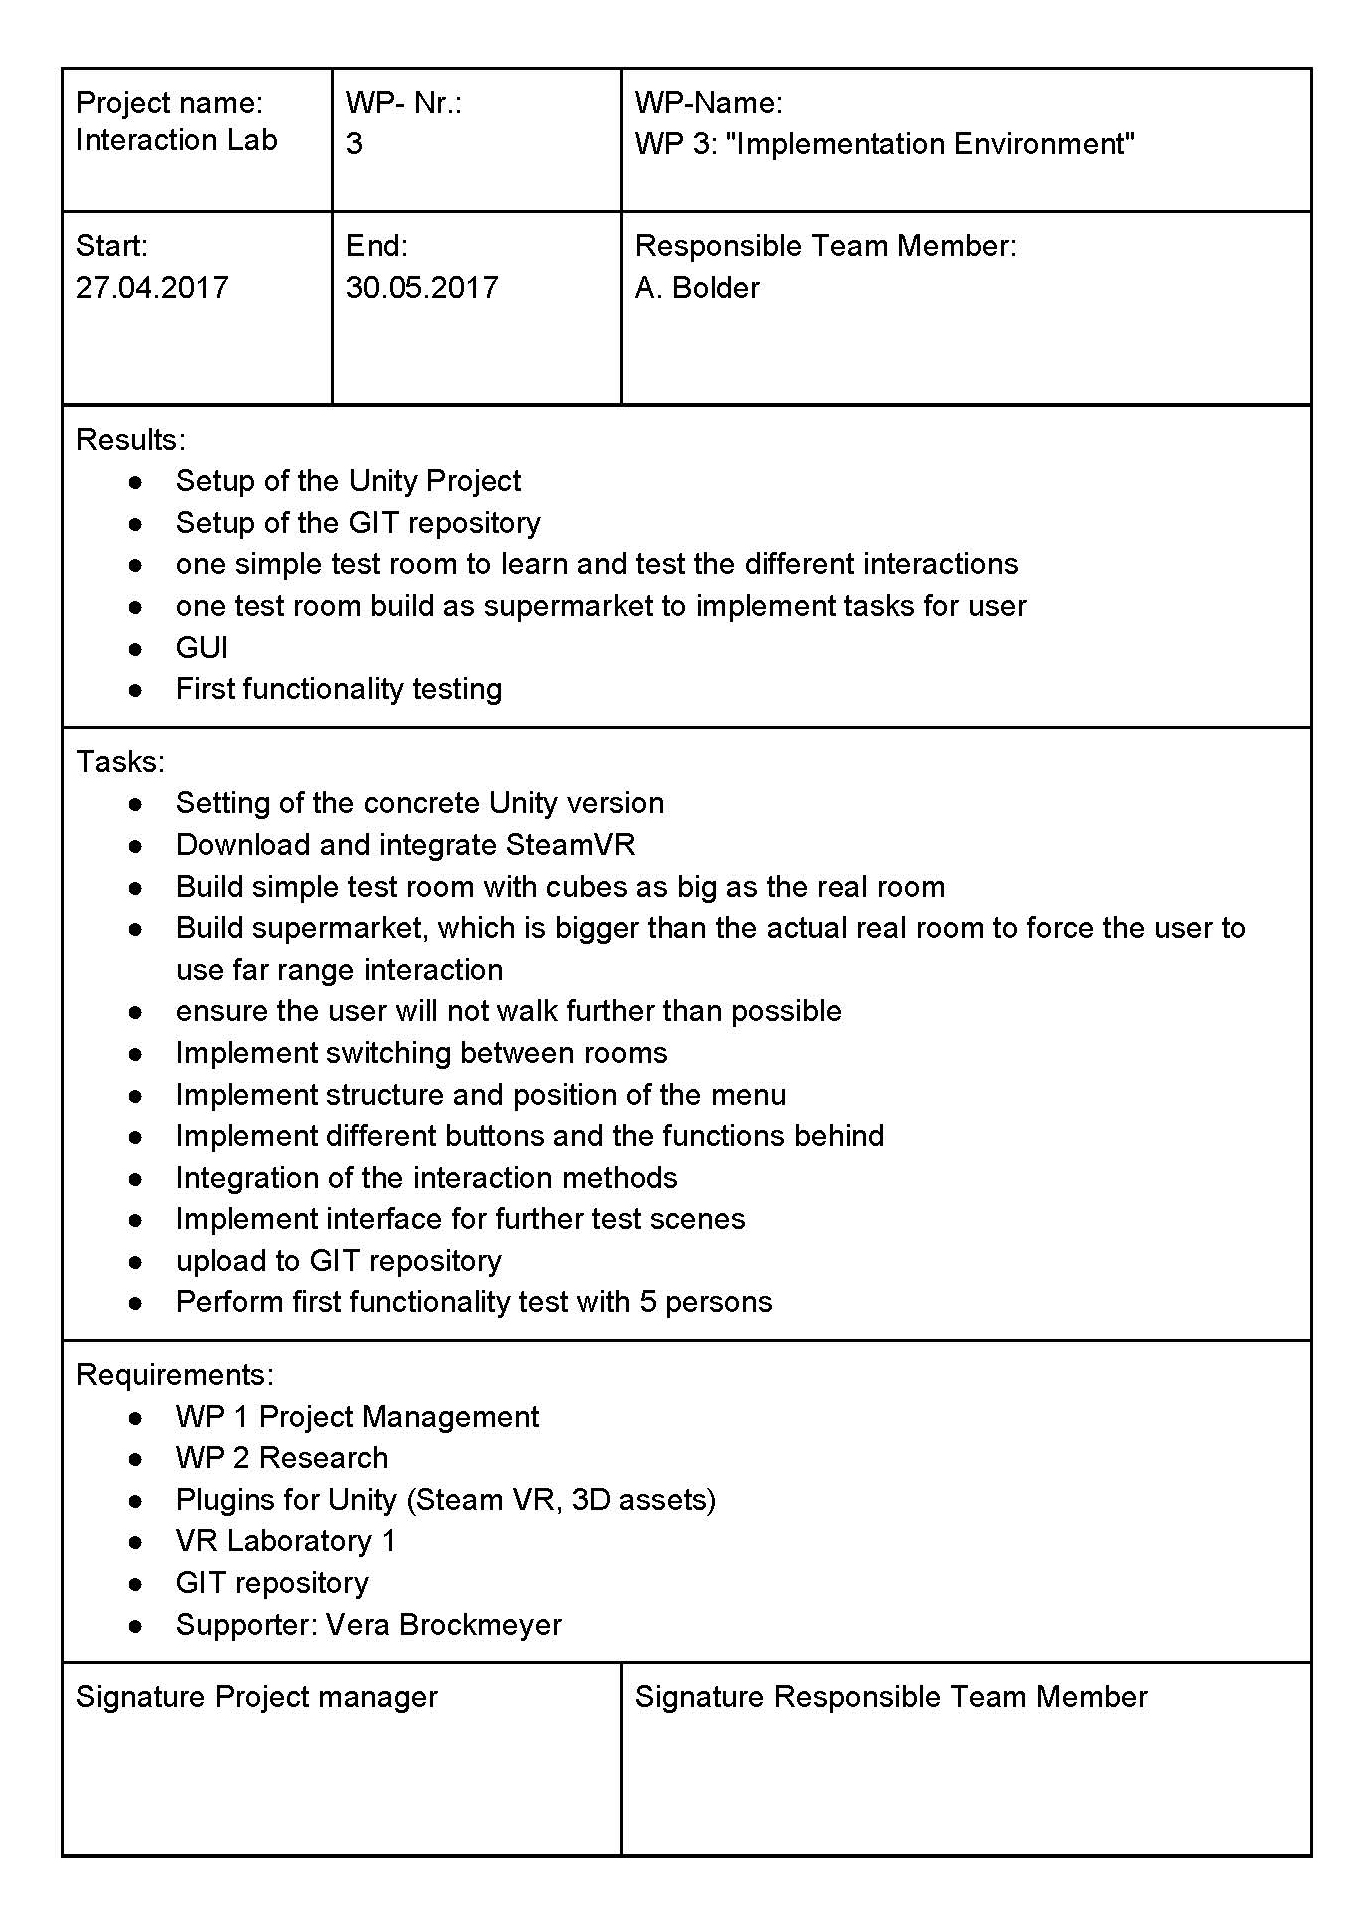
\includegraphics[width= 16 cm]{Images/Workpackages_Seite_3.jpg}			
	\caption[]{Third Workpackage: Implementation of the  Environment}
	\label{fig:Workpackage3}
\end{figure} 

\newpage
\begin{figure}[H] 
	\center 
	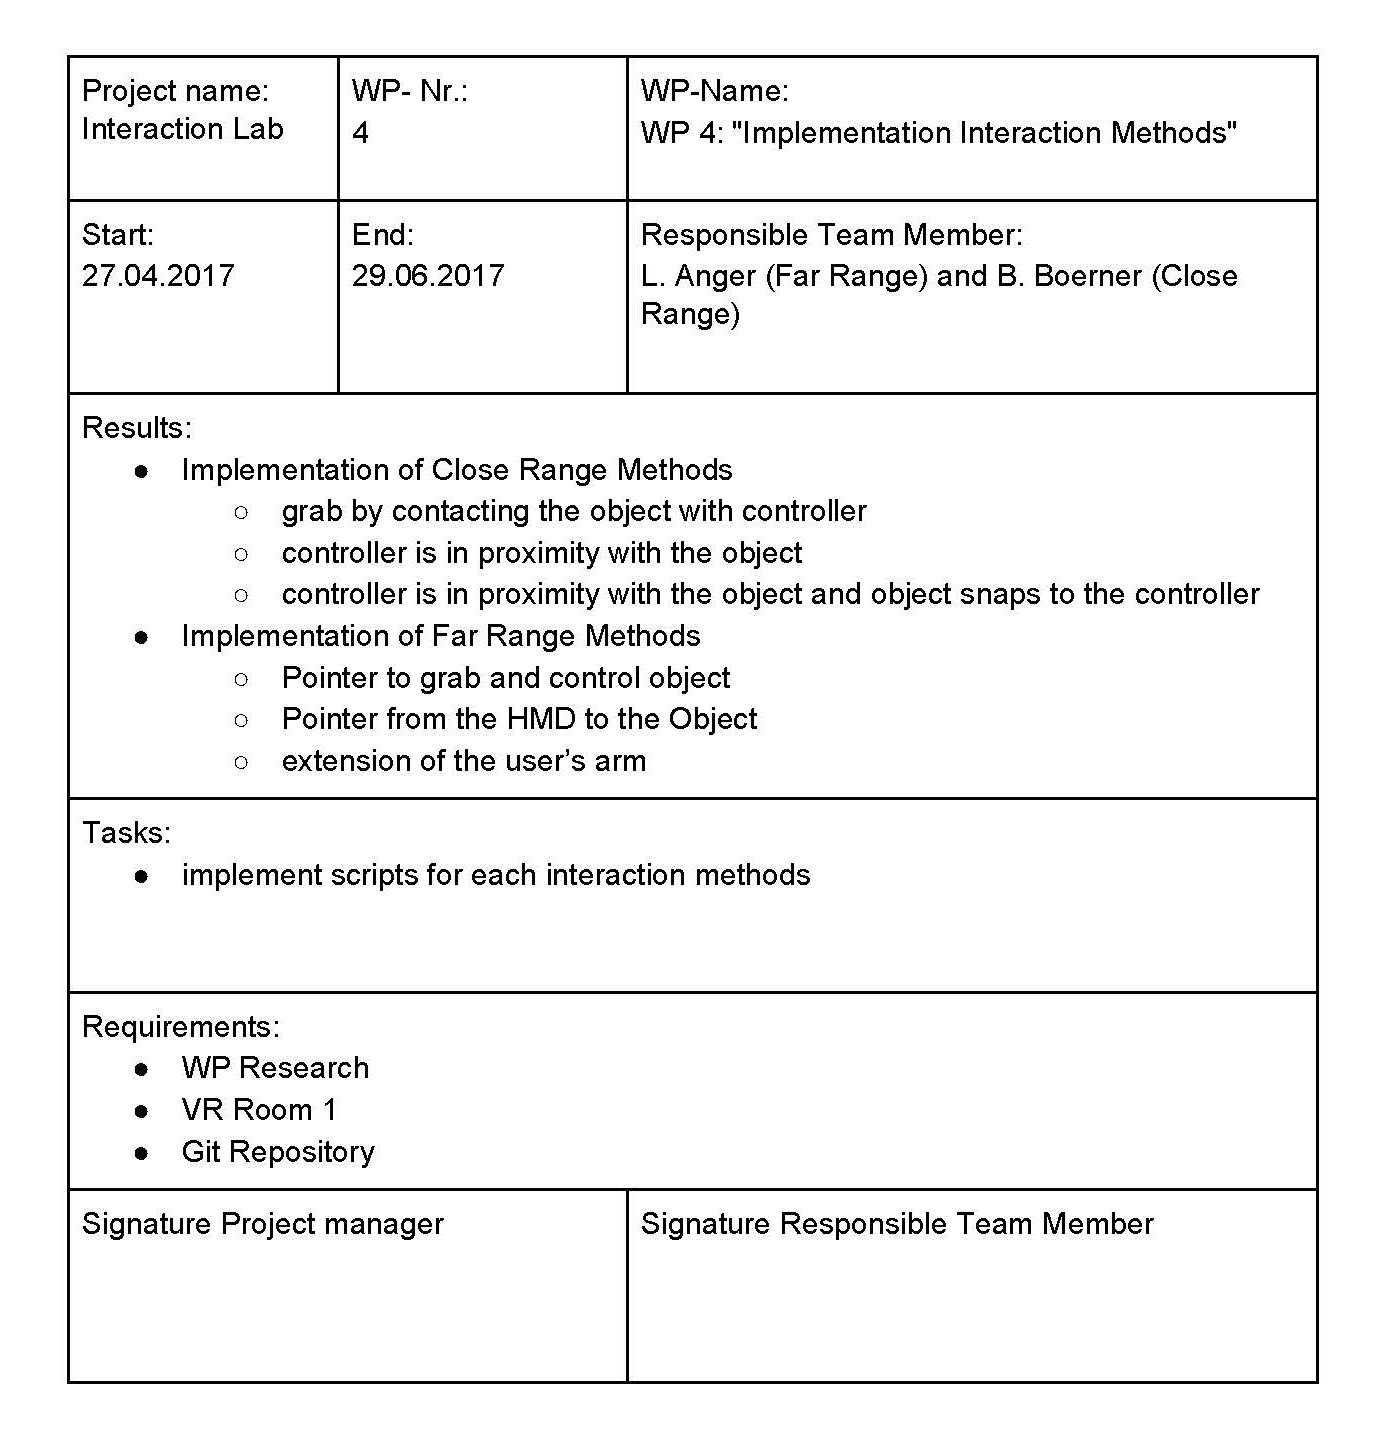
\includegraphics[width= 16 cm]{Images/Workpackages_Seite_4.jpg}			
	\caption[]{Forth Workpackage: Implementation of the  Interaction Methods}
	\label{fig:Workpackage4}
\end{figure} 

\newpage
\begin{figure}[H] 
	\center 
	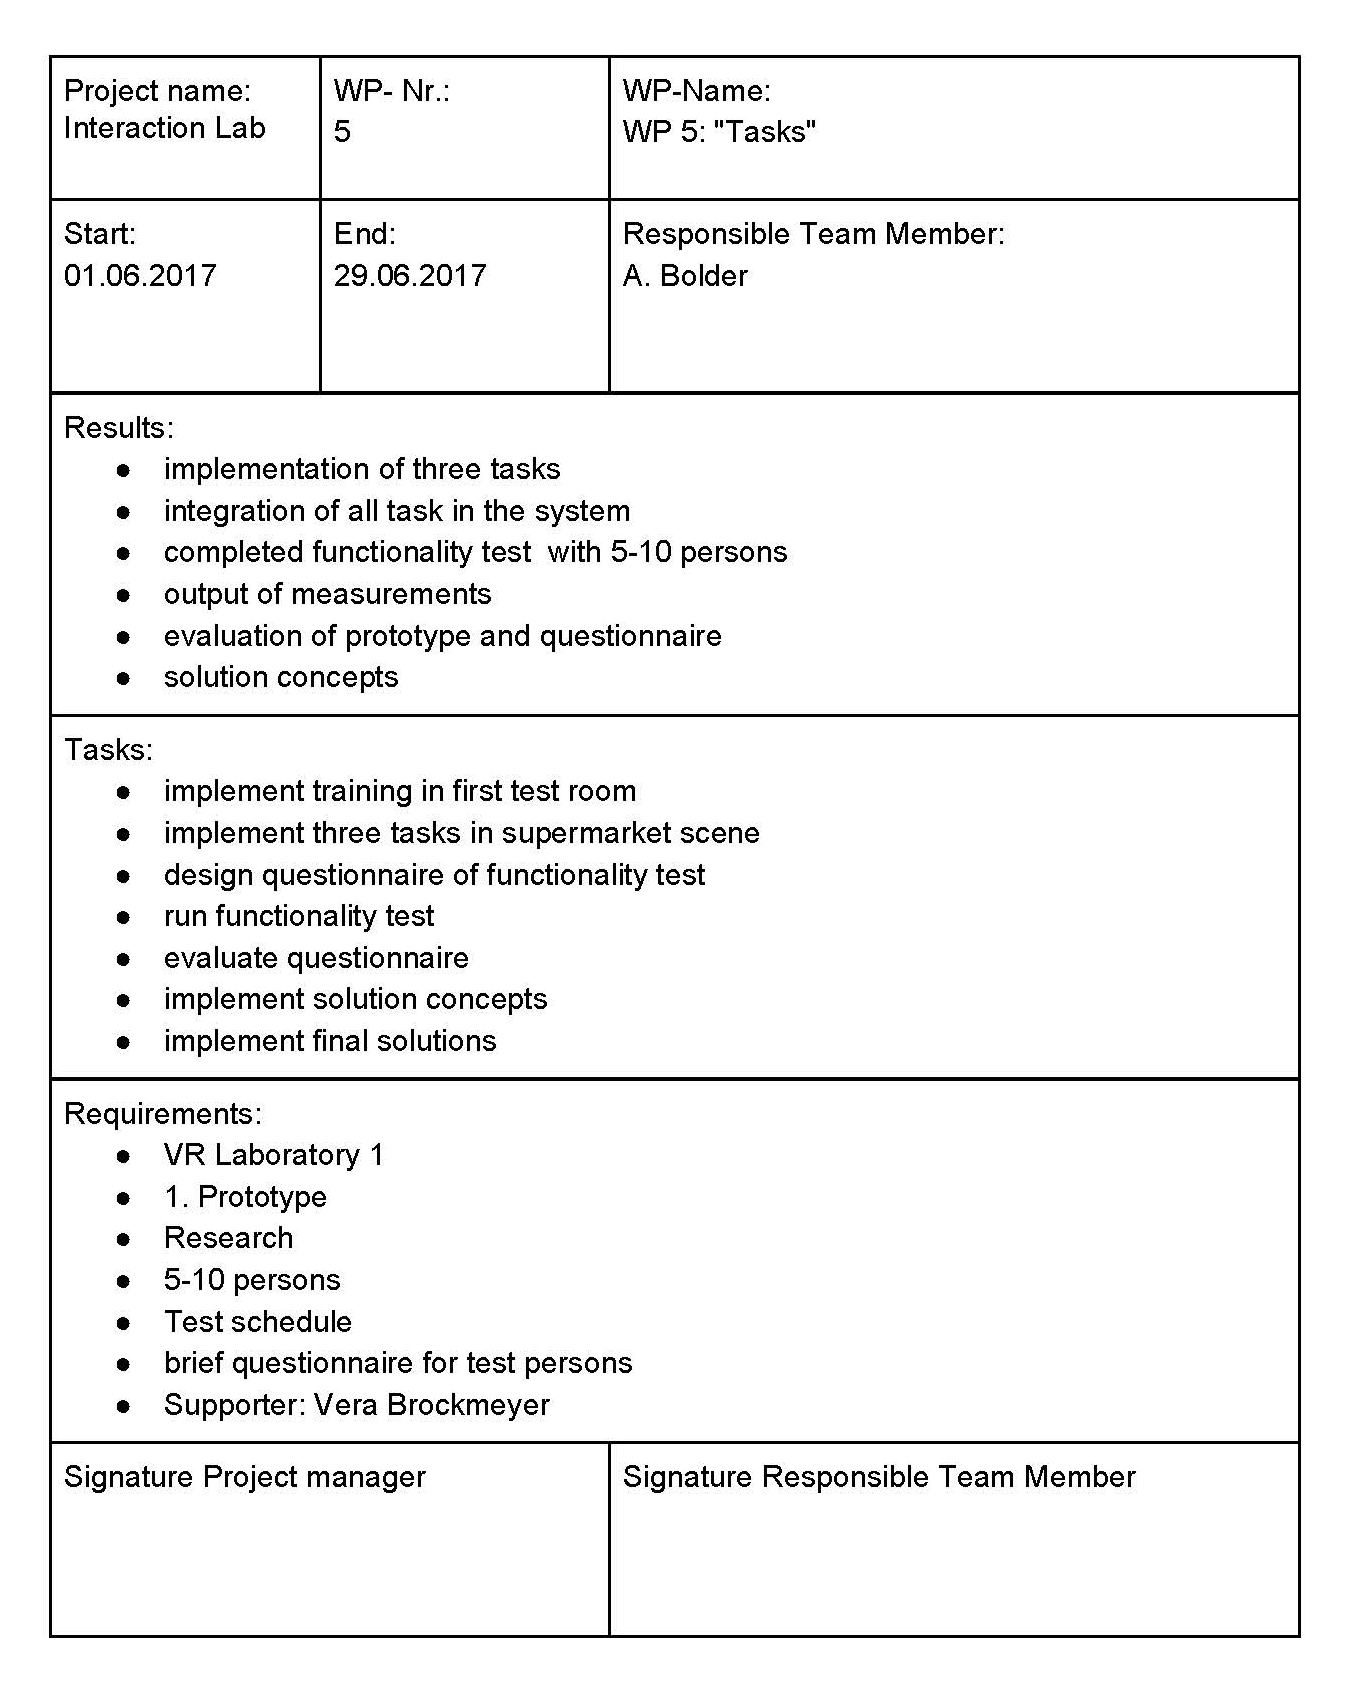
\includegraphics[width= 16 cm]{Images/Workpackages_Seite_5.jpg}			
	\caption[]{Fifth Workpackage: Tasks}
	\label{fig:Workpackage5}
\end{figure} 

\newpage
\begin{figure}[H] 
	\center 
	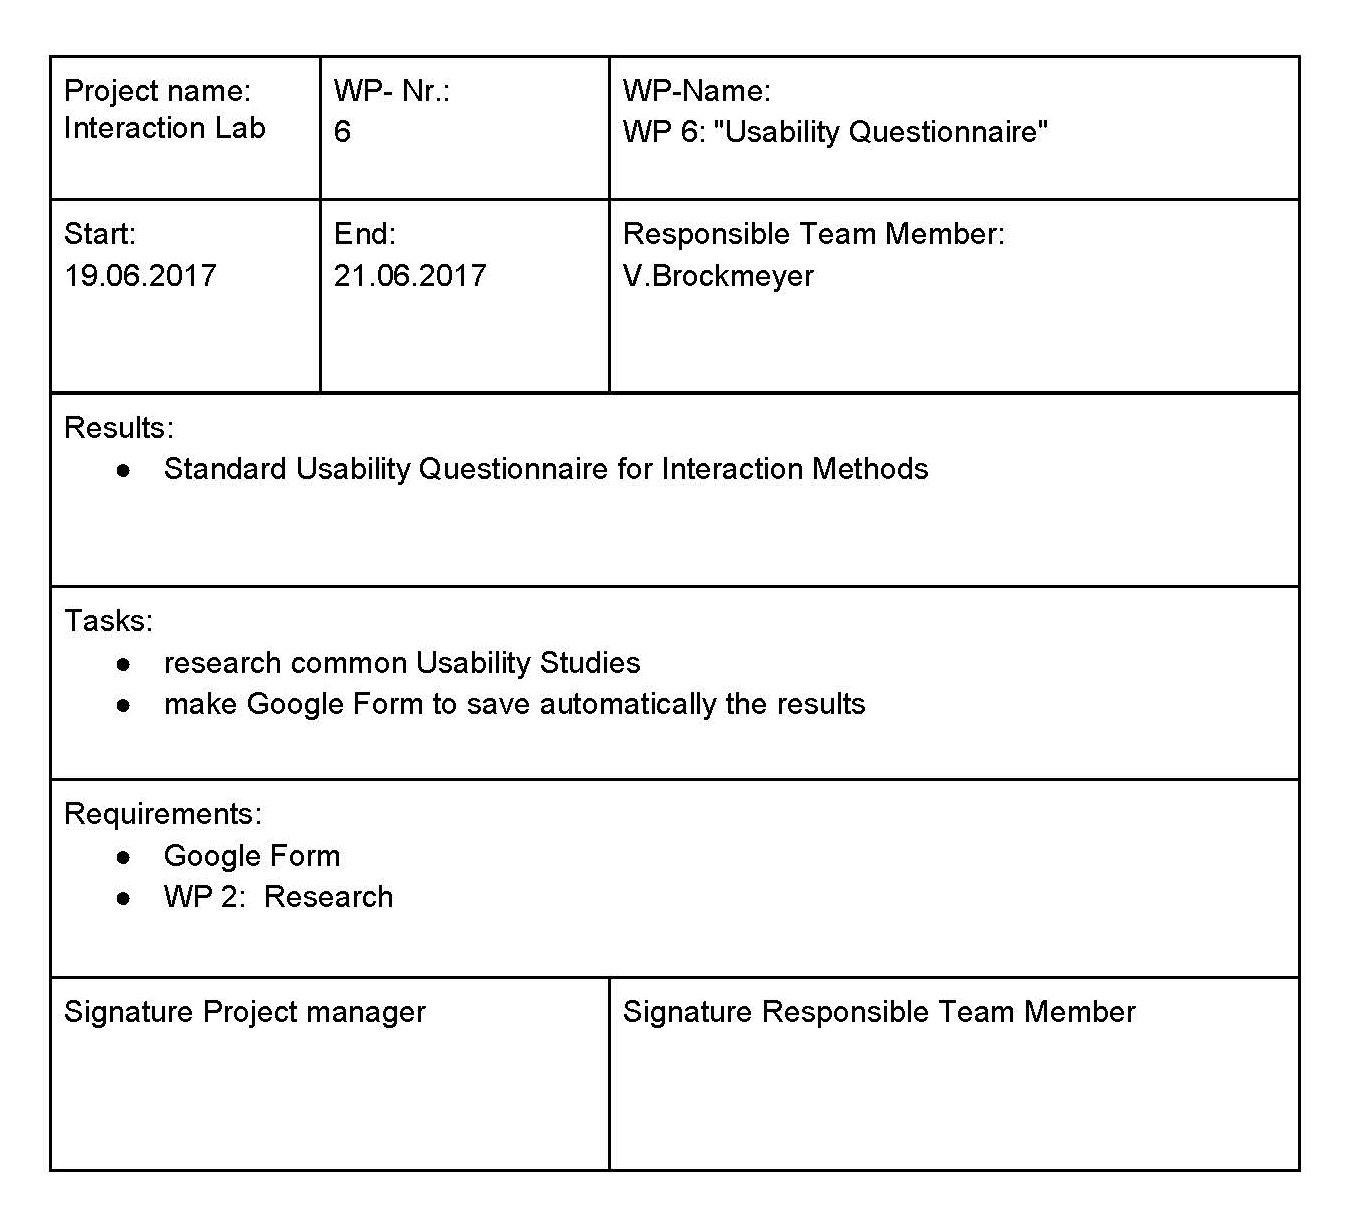
\includegraphics[width= 16 cm]{Images/Workpackages_Seite_6.jpg}			
	\caption[]{Sixth Workpackage: Usability Questionaire}
	\label{fig:Workpackage6}
\end{figure} 

\newpage
\begin{figure}[H] 
	\center 
	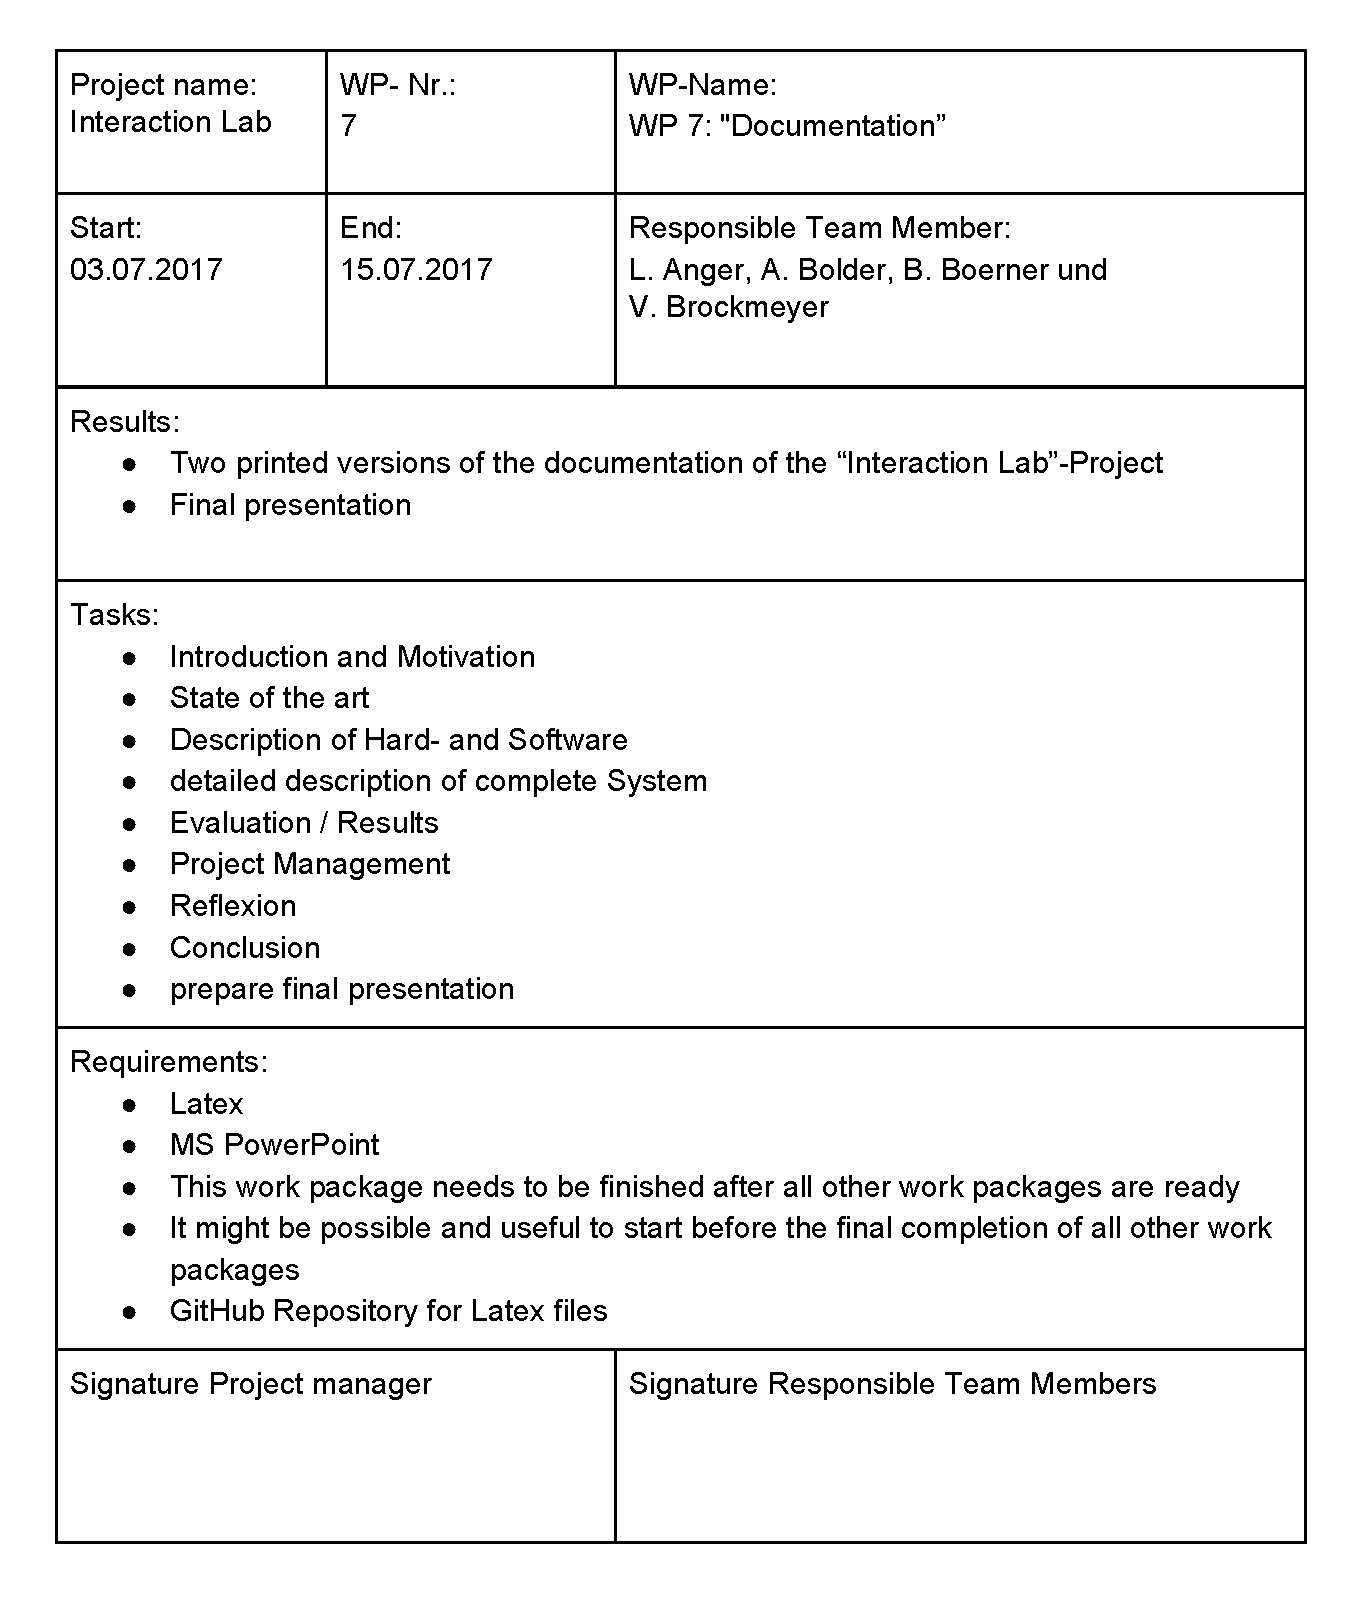
\includegraphics[width= 16 cm]{Images/Workpackages_Seite_7.jpg}			
	\caption[]{Seventh Workpackage: Documentation}
	\label{fig:Workpackage7}
\end{figure} 


\newpage
\begin{figure}[H] 
	\center 
	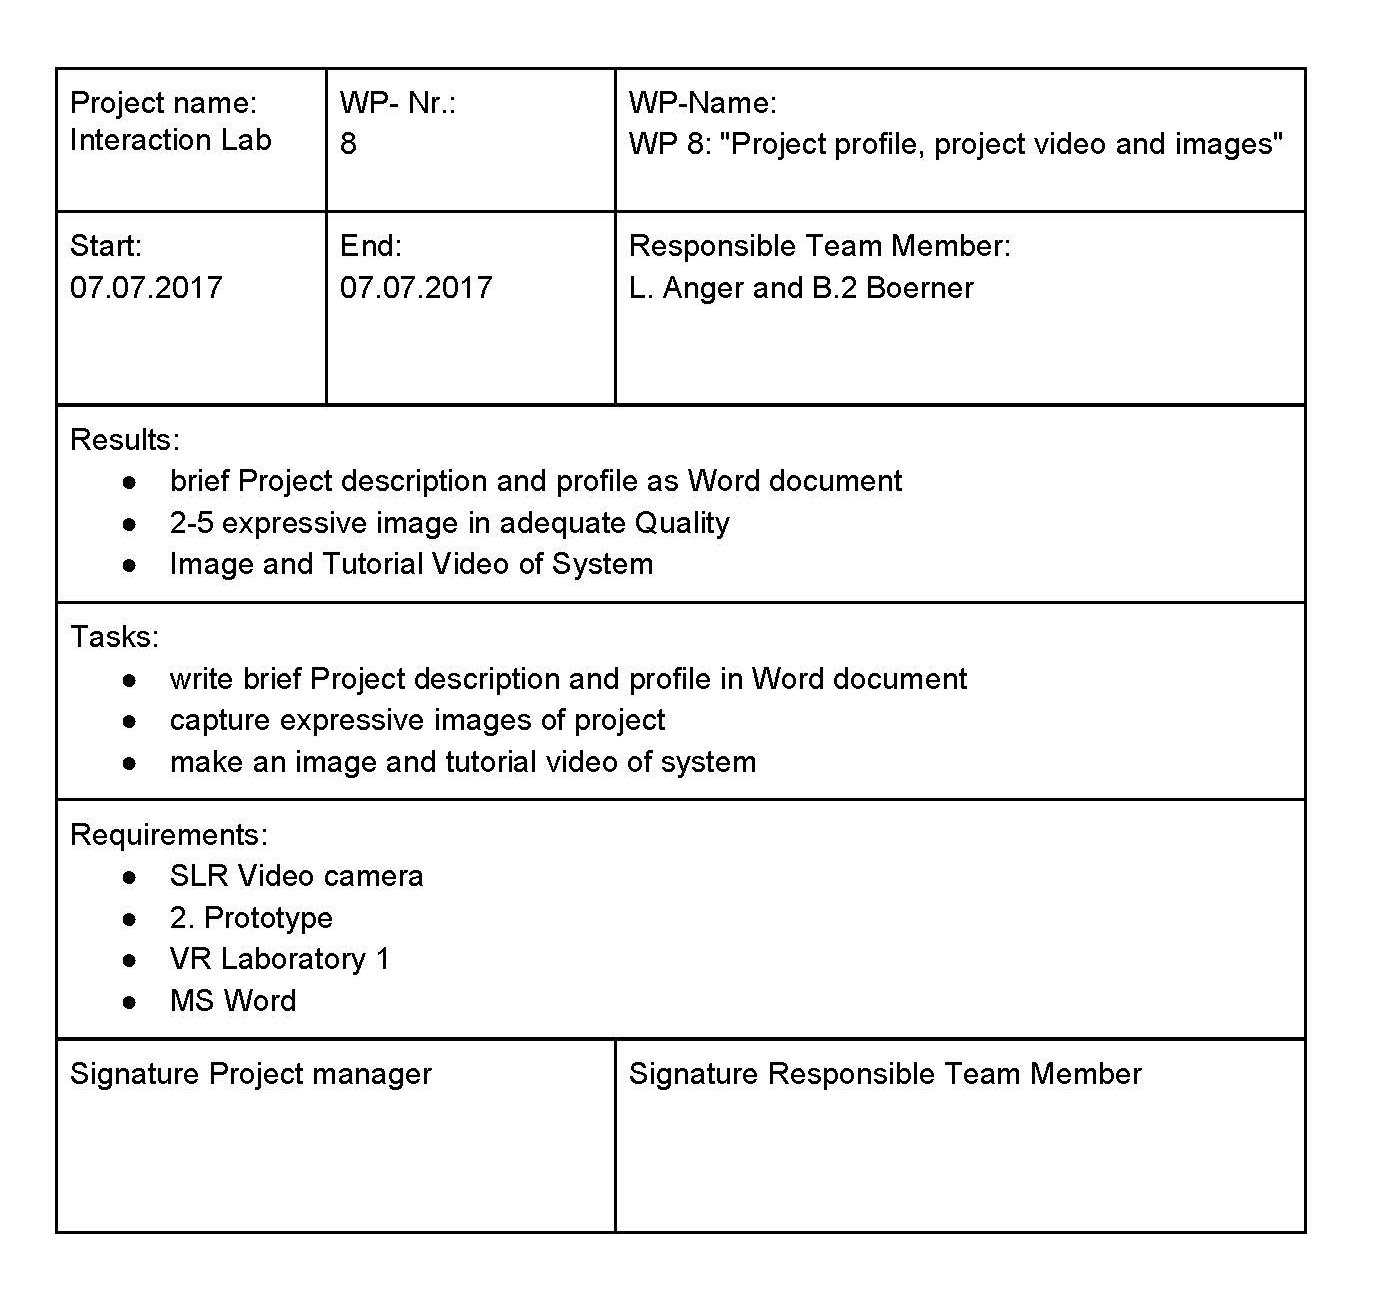
\includegraphics[width= 16 cm]{Images/Workpackages_Seite_8.jpg}			
	\caption[]{Eighth Workpackage: Project Profile, Video and Images}
	\label{fig:Workpackage8}
\end{figure} 




















\newpage
\bibliographystyle{plain}
\bibliography{main}
\end{document}